\documentclass[]{article}
\usepackage{lmodern}
\usepackage{amssymb,amsmath}
\usepackage{ifxetex,ifluatex}
\usepackage{fixltx2e} % provides \textsubscript
\ifnum 0\ifxetex 1\fi\ifluatex 1\fi=0 % if pdftex
  \usepackage[T1]{fontenc}
  \usepackage[utf8]{inputenc}
\else % if luatex or xelatex
  \ifxetex
    \usepackage{mathspec}
  \else
    \usepackage{fontspec}
  \fi
  \defaultfontfeatures{Ligatures=TeX,Scale=MatchLowercase}
  \newcommand{\euro}{€}
\fi
% use upquote if available, for straight quotes in verbatim environments
\IfFileExists{upquote.sty}{\usepackage{upquote}}{}
% use microtype if available
\IfFileExists{microtype.sty}{%
\usepackage{microtype}
\UseMicrotypeSet[protrusion]{basicmath} % disable protrusion for tt fonts
}{}
\usepackage[margin=1in]{geometry}
\usepackage{hyperref}
\PassOptionsToPackage{usenames,dvipsnames}{color} % color is loaded by hyperref
\hypersetup{unicode=true,
            pdftitle={Data Visualization in R with ggplot2},
            pdfborder={0 0 0},
            breaklinks=true}
\urlstyle{same}  % don't use monospace font for urls
\usepackage{color}
\usepackage{fancyvrb}
\newcommand{\VerbBar}{|}
\newcommand{\VERB}{\Verb[commandchars=\\\{\}]}
\DefineVerbatimEnvironment{Highlighting}{Verbatim}{commandchars=\\\{\}}
% Add ',fontsize=\small' for more characters per line
\usepackage{framed}
\definecolor{shadecolor}{RGB}{248,248,248}
\newenvironment{Shaded}{\begin{snugshade}}{\end{snugshade}}
\newcommand{\KeywordTok}[1]{\textcolor[rgb]{0.13,0.29,0.53}{\textbf{{#1}}}}
\newcommand{\DataTypeTok}[1]{\textcolor[rgb]{0.13,0.29,0.53}{{#1}}}
\newcommand{\DecValTok}[1]{\textcolor[rgb]{0.00,0.00,0.81}{{#1}}}
\newcommand{\BaseNTok}[1]{\textcolor[rgb]{0.00,0.00,0.81}{{#1}}}
\newcommand{\FloatTok}[1]{\textcolor[rgb]{0.00,0.00,0.81}{{#1}}}
\newcommand{\ConstantTok}[1]{\textcolor[rgb]{0.00,0.00,0.00}{{#1}}}
\newcommand{\CharTok}[1]{\textcolor[rgb]{0.31,0.60,0.02}{{#1}}}
\newcommand{\SpecialCharTok}[1]{\textcolor[rgb]{0.00,0.00,0.00}{{#1}}}
\newcommand{\StringTok}[1]{\textcolor[rgb]{0.31,0.60,0.02}{{#1}}}
\newcommand{\VerbatimStringTok}[1]{\textcolor[rgb]{0.31,0.60,0.02}{{#1}}}
\newcommand{\SpecialStringTok}[1]{\textcolor[rgb]{0.31,0.60,0.02}{{#1}}}
\newcommand{\ImportTok}[1]{{#1}}
\newcommand{\CommentTok}[1]{\textcolor[rgb]{0.56,0.35,0.01}{\textit{{#1}}}}
\newcommand{\DocumentationTok}[1]{\textcolor[rgb]{0.56,0.35,0.01}{\textbf{\textit{{#1}}}}}
\newcommand{\AnnotationTok}[1]{\textcolor[rgb]{0.56,0.35,0.01}{\textbf{\textit{{#1}}}}}
\newcommand{\CommentVarTok}[1]{\textcolor[rgb]{0.56,0.35,0.01}{\textbf{\textit{{#1}}}}}
\newcommand{\OtherTok}[1]{\textcolor[rgb]{0.56,0.35,0.01}{{#1}}}
\newcommand{\FunctionTok}[1]{\textcolor[rgb]{0.00,0.00,0.00}{{#1}}}
\newcommand{\VariableTok}[1]{\textcolor[rgb]{0.00,0.00,0.00}{{#1}}}
\newcommand{\ControlFlowTok}[1]{\textcolor[rgb]{0.13,0.29,0.53}{\textbf{{#1}}}}
\newcommand{\OperatorTok}[1]{\textcolor[rgb]{0.81,0.36,0.00}{\textbf{{#1}}}}
\newcommand{\BuiltInTok}[1]{{#1}}
\newcommand{\ExtensionTok}[1]{{#1}}
\newcommand{\PreprocessorTok}[1]{\textcolor[rgb]{0.56,0.35,0.01}{\textit{{#1}}}}
\newcommand{\AttributeTok}[1]{\textcolor[rgb]{0.77,0.63,0.00}{{#1}}}
\newcommand{\RegionMarkerTok}[1]{{#1}}
\newcommand{\InformationTok}[1]{\textcolor[rgb]{0.56,0.35,0.01}{\textbf{\textit{{#1}}}}}
\newcommand{\WarningTok}[1]{\textcolor[rgb]{0.56,0.35,0.01}{\textbf{\textit{{#1}}}}}
\newcommand{\AlertTok}[1]{\textcolor[rgb]{0.94,0.16,0.16}{{#1}}}
\newcommand{\ErrorTok}[1]{\textcolor[rgb]{0.64,0.00,0.00}{\textbf{{#1}}}}
\newcommand{\NormalTok}[1]{{#1}}
\usepackage{longtable,booktabs}
\usepackage{graphicx,grffile}
\makeatletter
\def\maxwidth{\ifdim\Gin@nat@width>\linewidth\linewidth\else\Gin@nat@width\fi}
\def\maxheight{\ifdim\Gin@nat@height>\textheight\textheight\else\Gin@nat@height\fi}
\makeatother
% Scale images if necessary, so that they will not overflow the page
% margins by default, and it is still possible to overwrite the defaults
% using explicit options in \includegraphics[width, height, ...]{}
\setkeys{Gin}{width=\maxwidth,height=\maxheight,keepaspectratio}
\setlength{\parindent}{0pt}
\setlength{\parskip}{6pt plus 2pt minus 1pt}
\setlength{\emergencystretch}{3em}  % prevent overfull lines
\providecommand{\tightlist}{%
  \setlength{\itemsep}{0pt}\setlength{\parskip}{0pt}}
\setcounter{secnumdepth}{5}

%%% Use protect on footnotes to avoid problems with footnotes in titles
\let\rmarkdownfootnote\footnote%
\def\footnote{\protect\rmarkdownfootnote}

%%% Change title format to be more compact
\usepackage{titling}

% Create subtitle command for use in maketitle
\newcommand{\subtitle}[1]{
  \posttitle{
    \begin{center}\large#1\end{center}
    }
}

\setlength{\droptitle}{-2em}
  \title{Data Visualization in R with ggplot2}
  \pretitle{\vspace{\droptitle}\centering\huge}
  \posttitle{\par}
  \author{}
  \preauthor{}\postauthor{}
  \date{}
  \predate{}\postdate{}


% Redefines (sub)paragraphs to behave more like sections
\ifx\paragraph\undefined\else
\let\oldparagraph\paragraph
\renewcommand{\paragraph}[1]{\oldparagraph{#1}\mbox{}}
\fi
\ifx\subparagraph\undefined\else
\let\oldsubparagraph\subparagraph
\renewcommand{\subparagraph}[1]{\oldsubparagraph{#1}\mbox{}}
\fi


\usepackage{amsthm}
\newtheorem{theorem}{Theorem}[section]
\newtheorem{lemma}{Lemma}[section]
\theoremstyle{definition}
\newtheorem{definition}{Definition}[section]
\newtheorem{corollary}{Corollary}[section]
\newtheorem{proposition}{Proposition}[section]
\theoremstyle{definition}
\newtheorem{example}{Example}[section]
\theoremstyle{definition}
\newtheorem{exercise}{Exercise}[section]
\theoremstyle{remark}
\newtheorem*{remark}{Remark}
\newtheorem*{solution}{Solution}
\begin{document}
\maketitle

{
\setcounter{tocdepth}{2}
\tableofcontents
}
\section{Introduction}\label{introduction}

This course introduces you to data visualization in R using the ggplot2
package. The ggplot2 package implements the grammar of graphics concepts
for creating visually appealing and professional looking graphics in R.
Basic knowledge of working with datasets in R is essential but
experience with plotting functions is not required.

By the end of the course you will be able to:

\begin{itemize}
\tightlist
\item
  Create scatterplots, histograms, line graphs, and boxplots
\item
  Add chart labels, axis labels and legends to the plots
\item
  Apply statistical transformations to the plots
\item
  Change various attributes of plot layers including color, shape, size
  and scale
\item
  Create mutiple plots in a single figure using facets
\item
  Apply themes to change the appearance of the plots
\end{itemize}

\begin{center}\rule{0.5\linewidth}{\linethickness}\end{center}

\emph{Last Updated: Oct 19, 2017 12:41 AM}

\section{Acknowledgments}\label{acknowledgments}

Content of this workshop is based on the following:

\begin{itemize}
\tightlist
\item
  \href{http://tutorials.iq.harvard.edu/R/Rgraphics/Rgraphics.html}{ggplot2
  tutorial from Harvard University}
\item
  \href{http://ggplot2.org/resources/2007-vanderbilt.pdf}{ggplot2
  Workshop (Vanderbilt, 2007)}
\end{itemize}

This work is licensed under a Creative Commons Attribution-ShareAlike
4.0 International License.

\section{Resources}\label{resources}

\begin{itemize}
\item
  \href{http://www.google.com}{Google}
\item
  \href{https://www.rstudio.com/wp-content/uploads/2015/03/ggplot2-cheatsheet.pdf}{Data
  Visualization with ggplot2 Cheat Sheet}
\item
  \href{http://docs.ggplot2.org}{ggplot2 Documentation}
\item
  \href{https://ase.tufts.edu/bugs/guide/assets/R\%20Graphics\%20Cookbook.pdf}{R
  Graphics Cookbook}
\item
  \href{http://tutorials.iq.harvard.edu/R/Rgraphics/Rgraphics.html}{ggplot2
  tutorial from Harvard University}
\item
  \href{http://ggplot2.org/resources/2007-vanderbilt.pdf}{ggplot2
  Workshop (Vanderbilt, 2007)}
\end{itemize}

\section{Getting Started}\label{getting-started}

\subsection{Prerequisites}\label{prerequisites}

Basic knowledge of working with datasets in R is essential. This course
assumes that you're comfortable with reading and manipulating datasets,
working with script files, and navigating in RStudio. Experience with
plotting functions in R is helpful but not required.

\subsection{Software Requirements}\label{software-requirements}

\subsubsection{R and RStudio}\label{r-and-rstudio}

Recent versions of R (version 3.2 or newer) and RStudio (version 0.99 or
above) are required.

You can download the latest versions from the links below:

\begin{itemize}
\tightlist
\item
  \href{https://cran.r-project.org}{Download R}
\item
  \href{https://www.rstudio.com/products/rstudio/download}{Download
  RStudio}
\end{itemize}

You can find out the version of R installed by typing \texttt{version}
at the console:

\begin{Shaded}
\begin{Highlighting}[]
\NormalTok{version}
\end{Highlighting}
\end{Shaded}

\begin{verbatim}
##                _                           
## platform       x86_64-pc-linux-gnu         
## arch           x86_64                      
## os             linux-gnu                   
## system         x86_64, linux-gnu           
## status                                     
## major          3                           
## minor          4.2                         
## year           2017                        
## month          01                          
## day            27                          
## svn rev        73369                       
## language       R                           
## version.string R version 3.4.2 (2017-01-27)
## nickname       Short Summer
\end{verbatim}

\subsection{Installing ggplot2}\label{installing-ggplot2}

If you don't have ggplot2 installed, you can install it using the
\texttt{install.packages()} function:

\begin{Shaded}
\begin{Highlighting}[]
\KeywordTok{install.packages}\NormalTok{(}\StringTok{"ggplot2"}\NormalTok{)}
\end{Highlighting}
\end{Shaded}

You can find out the version of ggplot installed using the
\texttt{packageVersion()} function:

\begin{Shaded}
\begin{Highlighting}[]
\KeywordTok{packageVersion}\NormalTok{(}\StringTok{"ggplot2"}\NormalTok{)}
\end{Highlighting}
\end{Shaded}

\begin{verbatim}
## [1] '2.2.1'
\end{verbatim}

\subsection{Installing ggplot2
Extentions}\label{installing-ggplot2-extentions}

We need the following ggplot extensions for this tutorial:

\begin{Shaded}
\begin{Highlighting}[]
\KeywordTok{install.packages}\NormalTok{(}\StringTok{"scales"}\NormalTok{)}
\KeywordTok{install.packages}\NormalTok{(}\StringTok{"ggrepel"}\NormalTok{)}
\KeywordTok{install.packages}\NormalTok{(}\StringTok{"ggthemes"}\NormalTok{)}
\end{Highlighting}
\end{Shaded}

\section{Grammer of Graphics}\label{grammer-of-graphics}

\begin{longtable}[c]{@{}ll@{}}
\toprule
\begin{minipage}[t]{0.59\columnwidth}\raggedright\strut
Wilkinson, L. (2006). \emph{The grammar of graphics}. Springer Science
\& Business Media.
\strut\end{minipage} &
\begin{minipage}[t]{0.21\columnwidth}\raggedright\strut
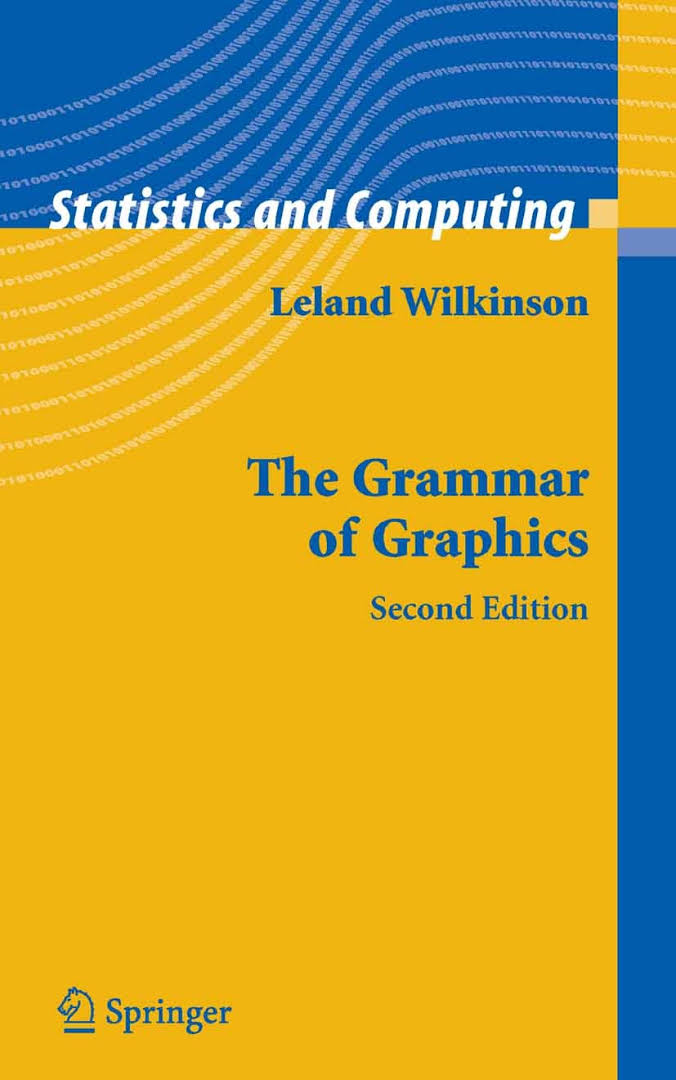
\includegraphics{./img/grammer_of_graphics.png}
\strut\end{minipage}\tabularnewline
\bottomrule
\end{longtable}

\subsection{Building Blocks of a
Graph}\label{building-blocks-of-a-graph}

\begin{itemize}
\tightlist
\item
  Data
\item
  Aesthetic mapping
\item
  Geometric object
\item
  Statistical transformations
\item
  Scales
\item
  Coordinate system
\item
  Position adjustments
\item
  Faceting
\end{itemize}

\begin{figure}[htbp]
\centering
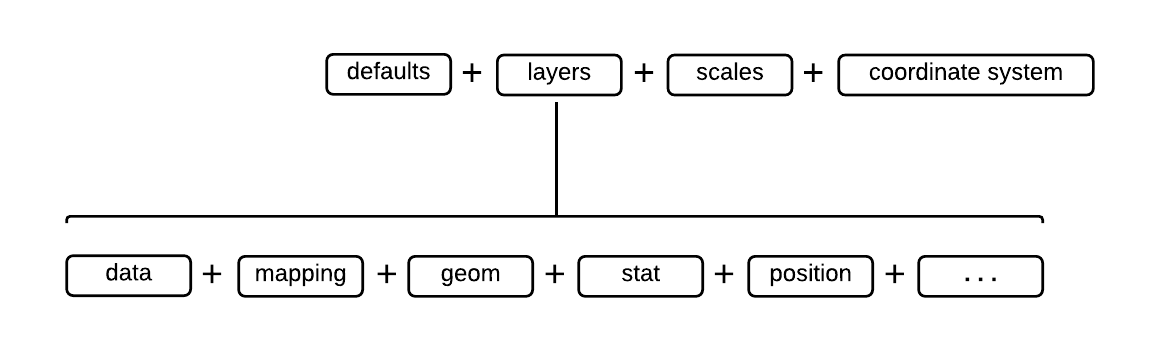
\includegraphics{./img/ggplot2_blocks.png}
\caption{}
\end{figure}

\section{Basic Plots}\label{basic-plots}

\subsection{Loading ggplot2}\label{loading-ggplot2}

Like any other R package, you must load \texttt{ggplot2} using the
\texttt{library} function before you can use any of the functionality
that it offers. We will also load the extensions that provide additional
features:

\begin{Shaded}
\begin{Highlighting}[]
\KeywordTok{library}\NormalTok{(ggplot2)}
\KeywordTok{library}\NormalTok{(ggrepel)}
\KeywordTok{library}\NormalTok{(ggthemes)}
\KeywordTok{library}\NormalTok{(scales)}
\end{Highlighting}
\end{Shaded}

\subsection{Dataset}\label{dataset}

Let's start by loading the housing dataset:

\begin{Shaded}
\begin{Highlighting}[]
\NormalTok{housing <-}\StringTok{ }\KeywordTok{read.csv}\NormalTok{(}\StringTok{"https://raw.githubusercontent.com/altaf-ali/ggplot_tutorial/master/data/housing.csv"}\NormalTok{)}
\end{Highlighting}
\end{Shaded}

Now, let's see what the dataset looks like:

\begin{Shaded}
\begin{Highlighting}[]
\KeywordTok{head}\NormalTok{(housing)}
\end{Highlighting}
\end{Shaded}

\begin{verbatim}
##   State Region       Date Home.Value Structure.Cost Land.Value
## 1    AK   West 2010-03-01     224952         160599      64352
## 2    AK   West 2010-06-01     225511         160252      65259
## 3    AK   West 2009-09-01     225820         163791      62029
## 4    AK   West 2009-12-01     224994         161787      63207
## 5    AK   West 2007-12-01     234590         155400      79190
## 6    AK   West 2008-03-01     233714         157458      76256
##   Land.Share..Pct. Home.Price.Index Land.Price.Index Year Quarter
## 1             28.6            1.481            1.552 2010       1
## 2             28.9            1.484            1.576 2010       2
## 3             27.5            1.486            1.494 2009       3
## 4             28.1            1.481            1.524 2009       4
## 5             33.8            1.544            1.885 2007       4
## 6             32.6            1.538            1.817 2008       1
\end{verbatim}

When dealing with date and time values, it's generally a good idea to
convert them to the appropriate data type.

\begin{Shaded}
\begin{Highlighting}[]
\NormalTok{housing$Date <-}\StringTok{ }\KeywordTok{as.Date}\NormalTok{(housing$Date)}
\end{Highlighting}
\end{Shaded}

Next, we create two subsets of the data, one with housing prices only
from New York, and another one with housing prices from 9 states in the
North East.

\begin{Shaded}
\begin{Highlighting}[]
\NormalTok{newyork <-}\StringTok{ }\KeywordTok{subset}\NormalTok{(housing, State ==}\StringTok{ "NY"}\NormalTok{)}
\NormalTok{northeast <-}\StringTok{ }\KeywordTok{subset}\NormalTok{(housing, Region ==}\StringTok{ "N. East"}\NormalTok{)}
\end{Highlighting}
\end{Shaded}

\subsection{Scatter Plot}\label{scatter-plot}

Now we're ready to plot. Everything starts with the \texttt{ggplot()}
function which creates a plot object. The two arguments passed to
\texttt{ggplot()} are:

\begin{longtable}[c]{@{}ll@{}}
\toprule
\begin{minipage}[b]{0.13\columnwidth}\raggedright\strut
Argument
\strut\end{minipage} &
\begin{minipage}[b]{0.80\columnwidth}\raggedright\strut
Description
\strut\end{minipage}\tabularnewline
\midrule
\endhead
\begin{minipage}[t]{0.13\columnwidth}\raggedright\strut
\texttt{data}
\strut\end{minipage} &
\begin{minipage}[t]{0.80\columnwidth}\raggedright\strut
Dataset for the plot. It should be a data.frame or something that can be
converted to data.frame
\strut\end{minipage}\tabularnewline
\begin{minipage}[t]{0.13\columnwidth}\raggedright\strut
\texttt{mapping}
\strut\end{minipage} &
\begin{minipage}[t]{0.80\columnwidth}\raggedright\strut
Aesthetic mappings for the plot
\strut\end{minipage}\tabularnewline
\bottomrule
\end{longtable}

Using the \texttt{newyork} dataset, let's create a scatter plot with
\texttt{Date} on the x-axis and \texttt{Home.Value} on the y-axis.

\begin{Shaded}
\begin{Highlighting}[]
\KeywordTok{ggplot}\NormalTok{(newyork, }\KeywordTok{aes}\NormalTok{(}\DataTypeTok{x =} \NormalTok{Date, }\DataTypeTok{y =} \NormalTok{Home.Value)) +}
\StringTok{  }\KeywordTok{geom_point}\NormalTok{()}
\end{Highlighting}
\end{Shaded}

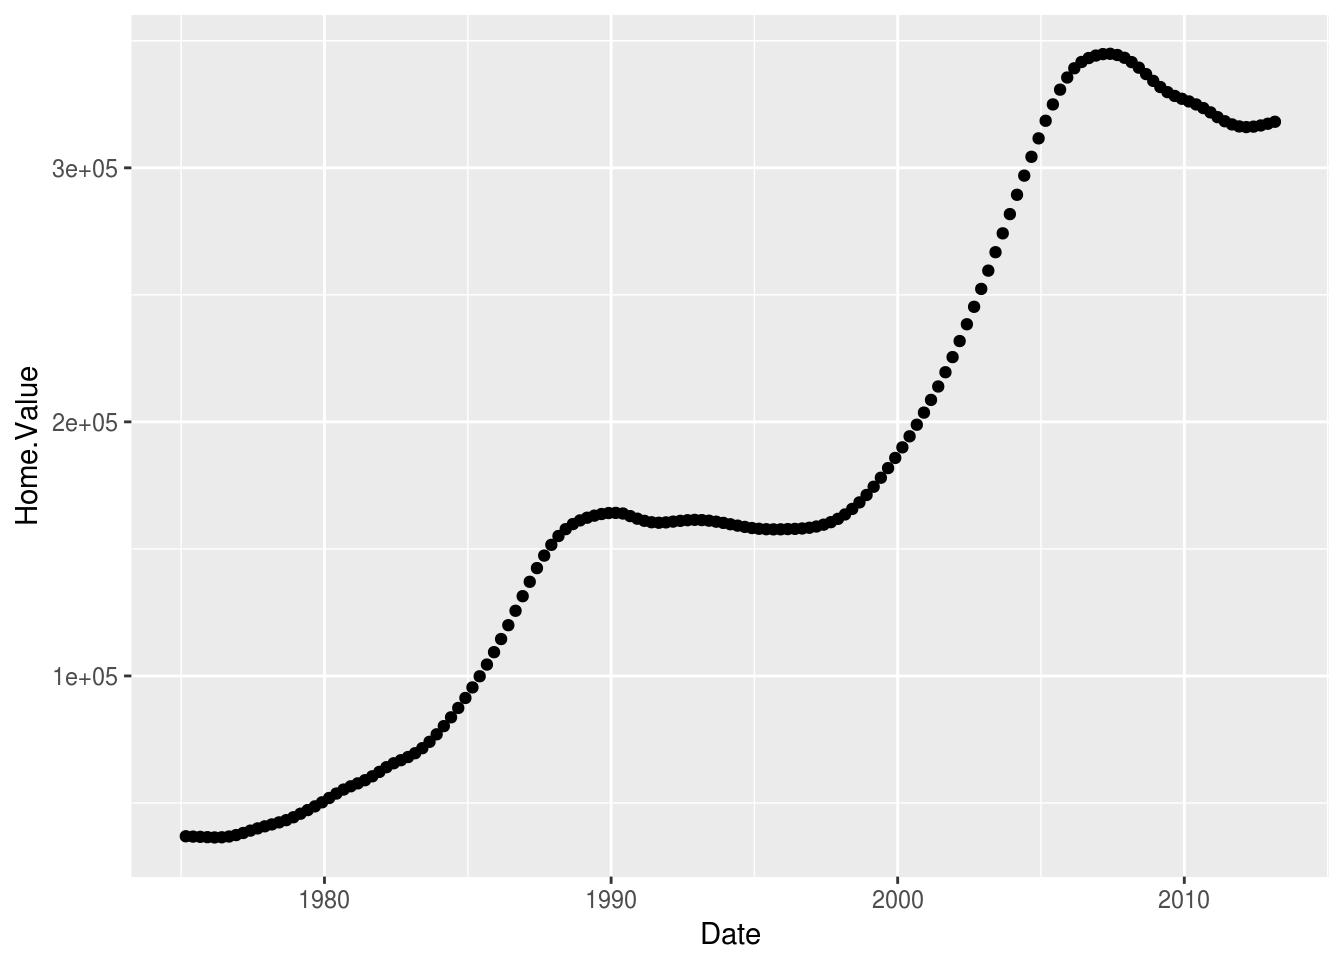
\includegraphics{ggplot_tutorial_files/figure-latex/unnamed-chunk-10-1.pdf}

Now let's see which ggplot building blocks are active in the above
example:

\begin{figure}[htbp]
\centering
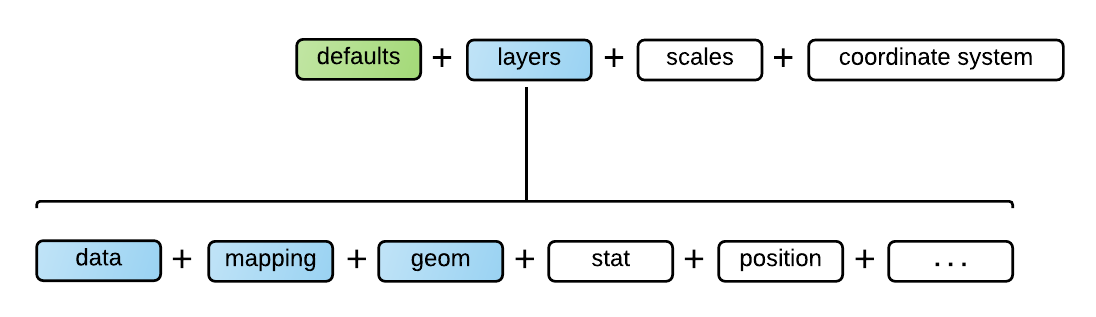
\includegraphics{./img/ggplot2_basics.png}
\caption{}
\end{figure}

\begin{longtable}[c]{@{}ll@{}}
\toprule
Data & \texttt{newyork}\tabularnewline
Mapping & \texttt{aes(x\ =\ Date,\ y\ =\ Home.Value)}\tabularnewline
Geom & \texttt{geom\_point()}\tabularnewline
\bottomrule
\end{longtable}

\subsection{Exercise}\label{exercise}

Use the
\href{https://www.rstudio.com/wp-content/uploads/2015/03/ggplot2-cheatsheet.pdf}{Data
Visualization with ggplot2 Cheat Sheet} or any other resource to find
out how to complete the exercises.

\begin{enumerate}
\def\labelenumi{\arabic{enumi}.}
\item
  Create a histogram of \texttt{Home.Value} using the \texttt{housing}
  data.

  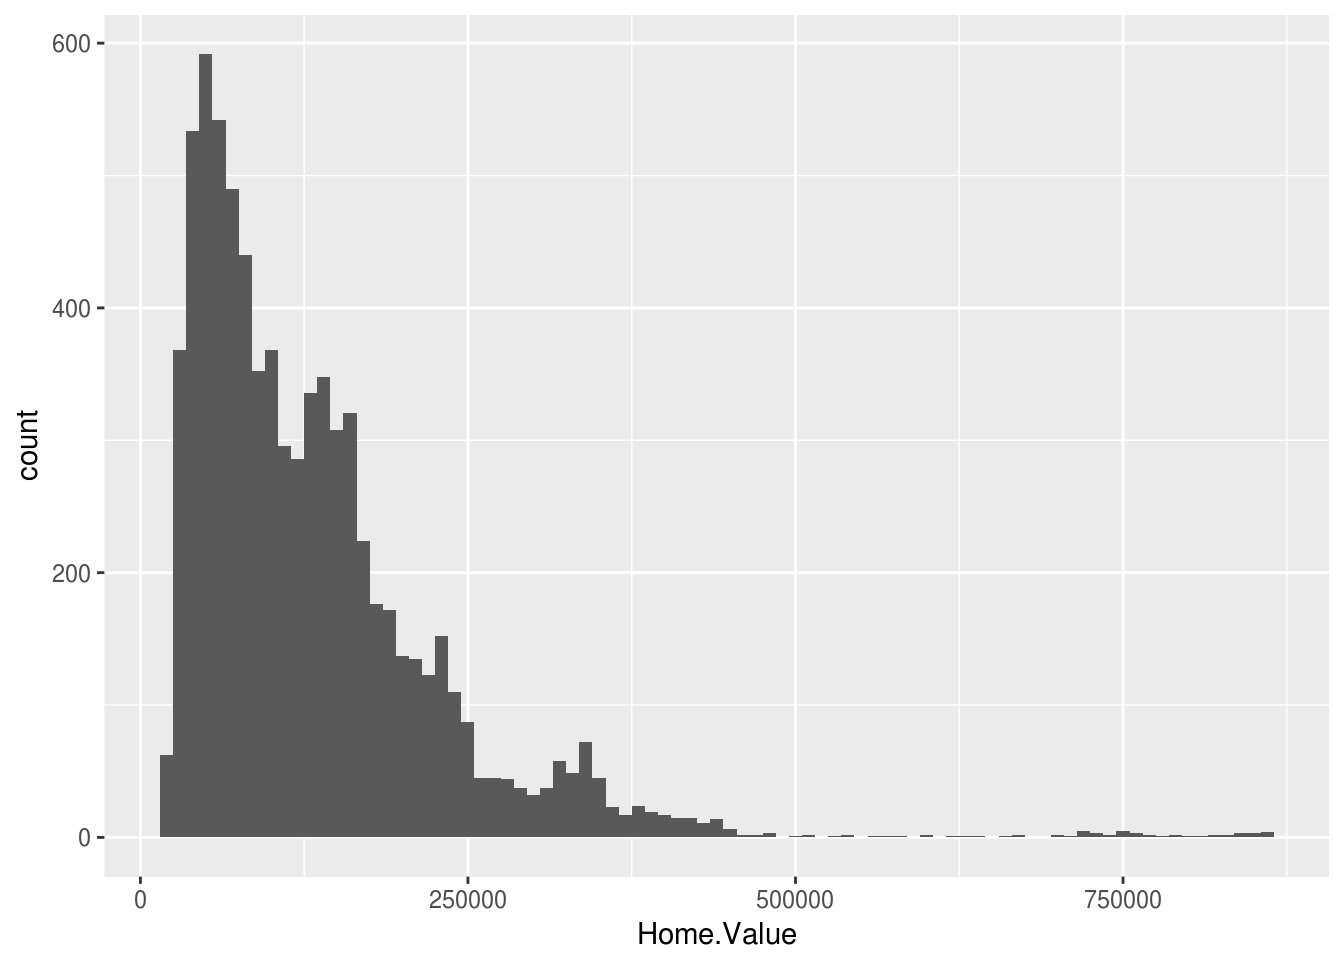
\includegraphics{ggplot_tutorial_files/figure-latex/unnamed-chunk-11-1.pdf}
\item
  Create a box plot of \texttt{Home.Value} using \texttt{northeast}
  dataset with \texttt{State} on the x-axis

  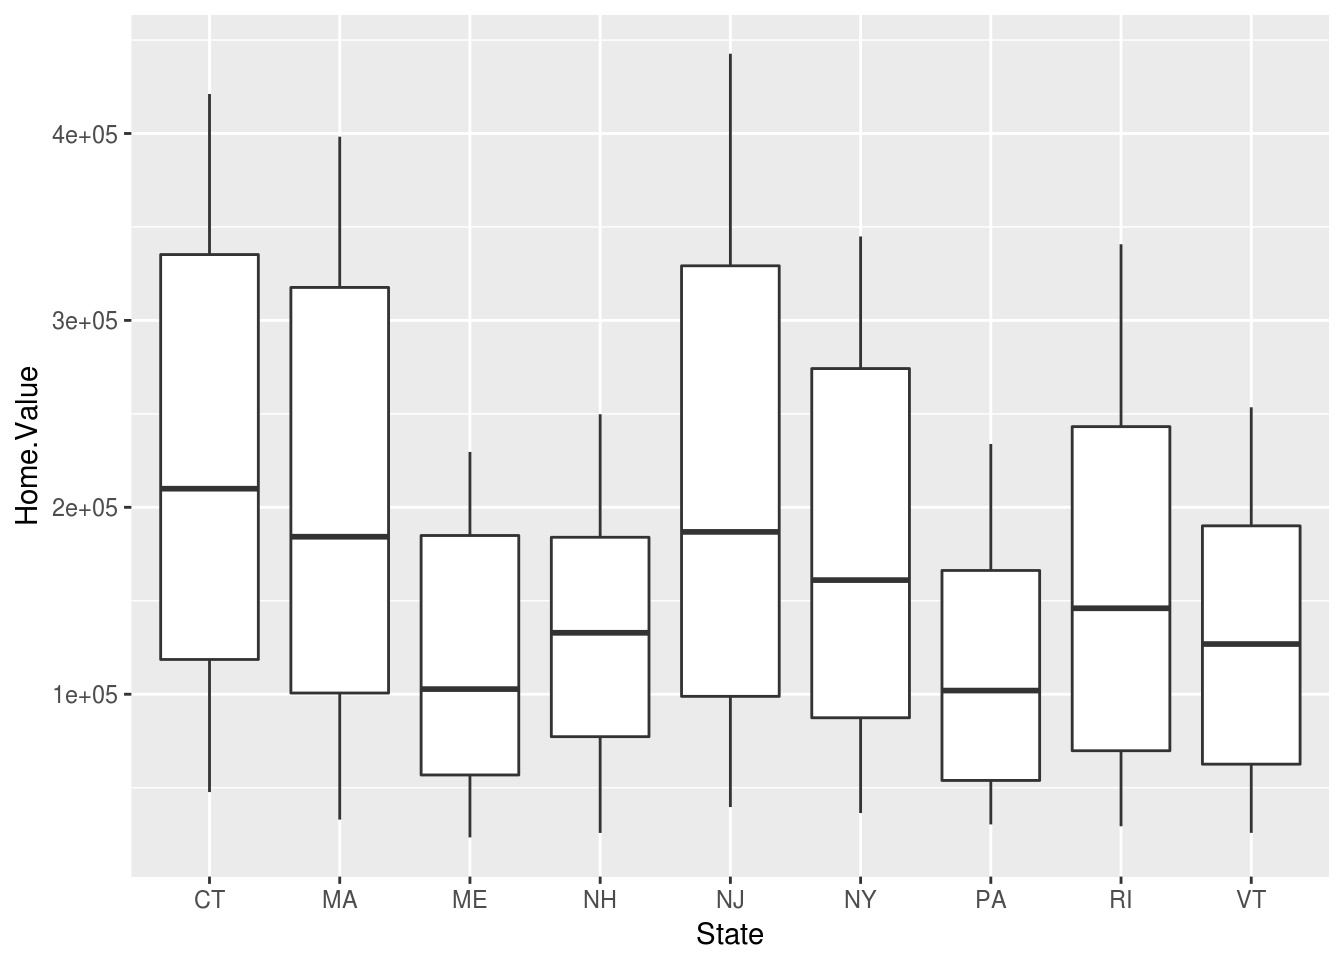
\includegraphics{ggplot_tutorial_files/figure-latex/unnamed-chunk-12-1.pdf}
\item
  Create a line plot using \texttt{newyork} dataset with \texttt{Date}
  on the x-axis and \texttt{Home.Value} on the y-axis

  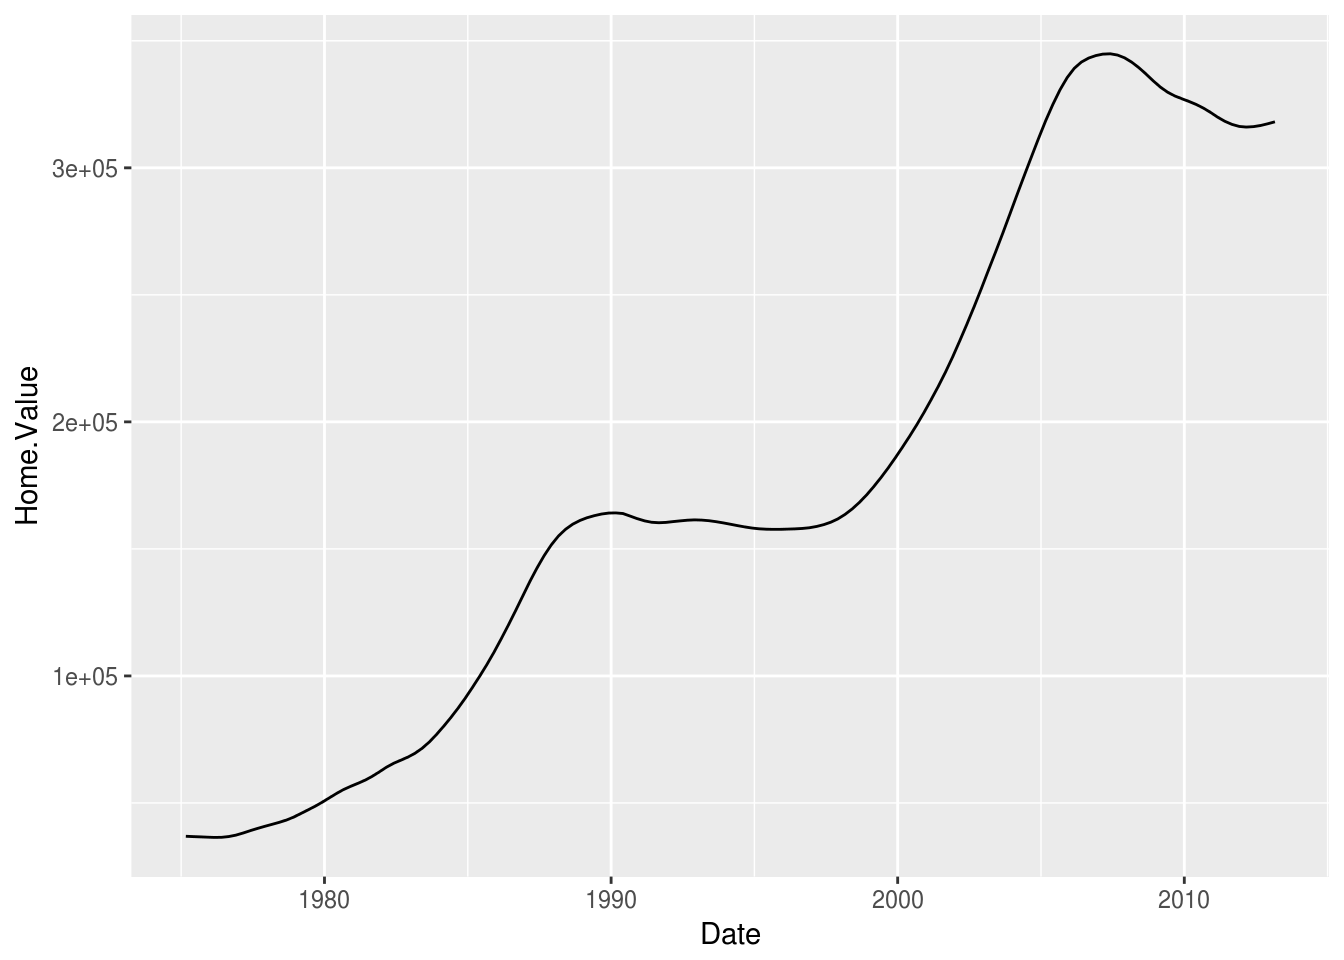
\includegraphics{ggplot_tutorial_files/figure-latex/unnamed-chunk-13-1.pdf}
\item
  Create a line plot using \texttt{northeast} dataset with \texttt{Date}
  on the x-axis and \texttt{Home.Value} on the y-axis and use a
  different color for each state

  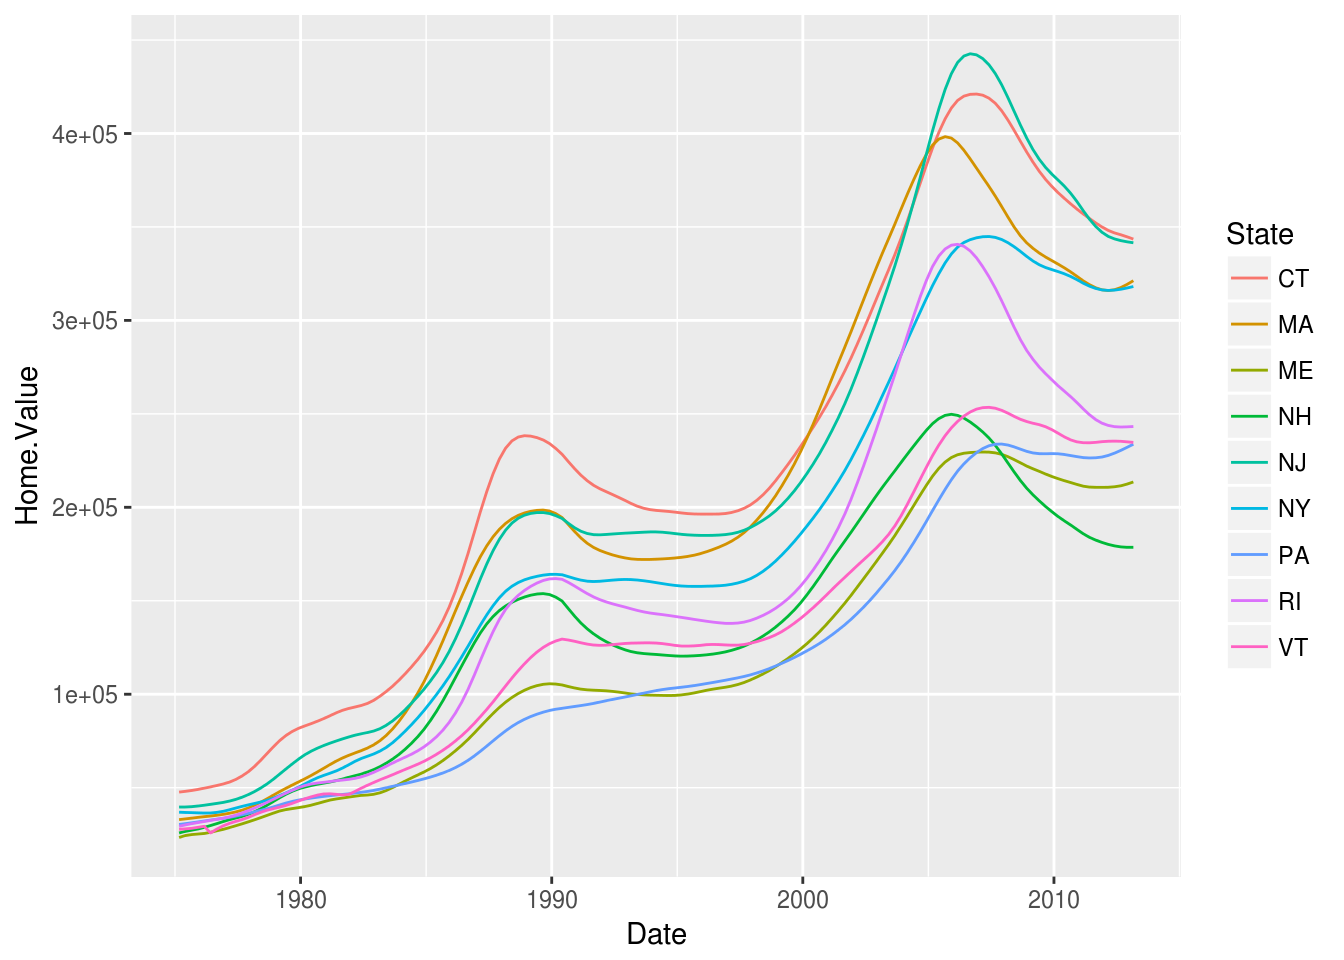
\includegraphics{ggplot_tutorial_files/figure-latex/unnamed-chunk-14-1.pdf}
\end{enumerate}

\section{Geoms and Statistics}\label{geoms-and-statistics}

Geometric objects (geoms) define the basic shape of the elements on the
plot.

\begin{itemize}
\tightlist
\item
  Every geom has a default statistic
\item
  Every statistic has a default geom
\end{itemize}

You can get a list of all geoms using the online help in RStudio

\begin{Shaded}
\begin{Highlighting}[]
\KeywordTok{help.search}\NormalTok{(}\StringTok{"geom_"}\NormalTok{, }\DataTypeTok{package =} \StringTok{"ggplot2"}\NormalTok{)}
\end{Highlighting}
\end{Shaded}

Change the size of each bin:

\begin{Shaded}
\begin{Highlighting}[]
\KeywordTok{ggplot}\NormalTok{(housing, }\KeywordTok{aes}\NormalTok{(}\DataTypeTok{x =} \NormalTok{Home.Value)) +}
\StringTok{  }\KeywordTok{geom_histogram}\NormalTok{(}\DataTypeTok{binwidth =} \DecValTok{1000}\NormalTok{)}
\end{Highlighting}
\end{Shaded}

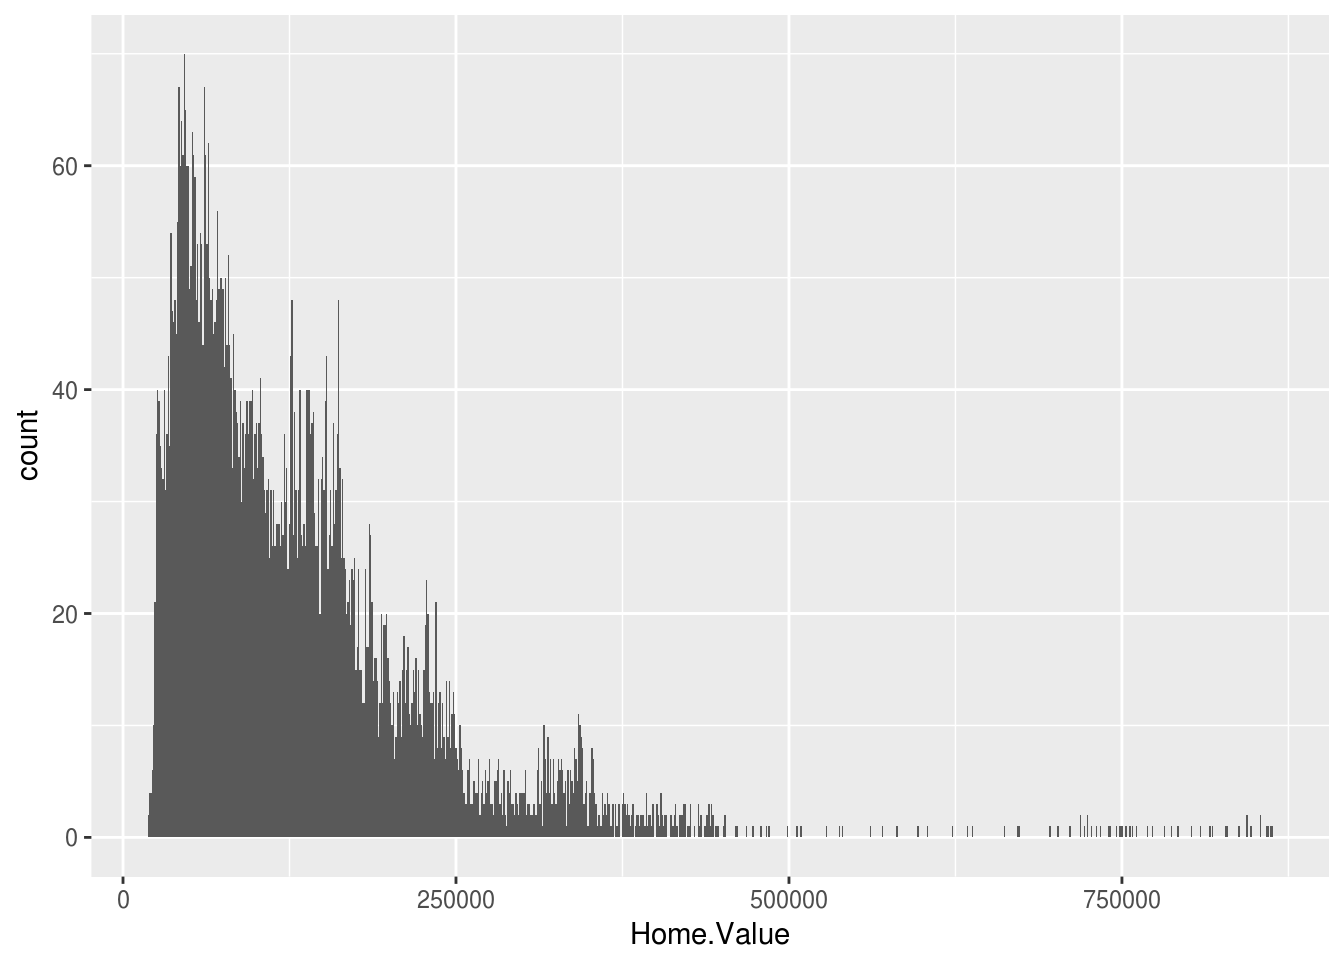
\includegraphics{ggplot_tutorial_files/figure-latex/unnamed-chunk-16-1.pdf}

Add a mapping for the fill color:

\begin{Shaded}
\begin{Highlighting}[]
\KeywordTok{ggplot}\NormalTok{(housing, }\KeywordTok{aes}\NormalTok{(}\DataTypeTok{x =} \NormalTok{Home.Value, }\DataTypeTok{fill =} \NormalTok{Region)) +}
\StringTok{  }\KeywordTok{geom_histogram}\NormalTok{(}\DataTypeTok{binwidth =} \DecValTok{1000}\NormalTok{)}
\end{Highlighting}
\end{Shaded}

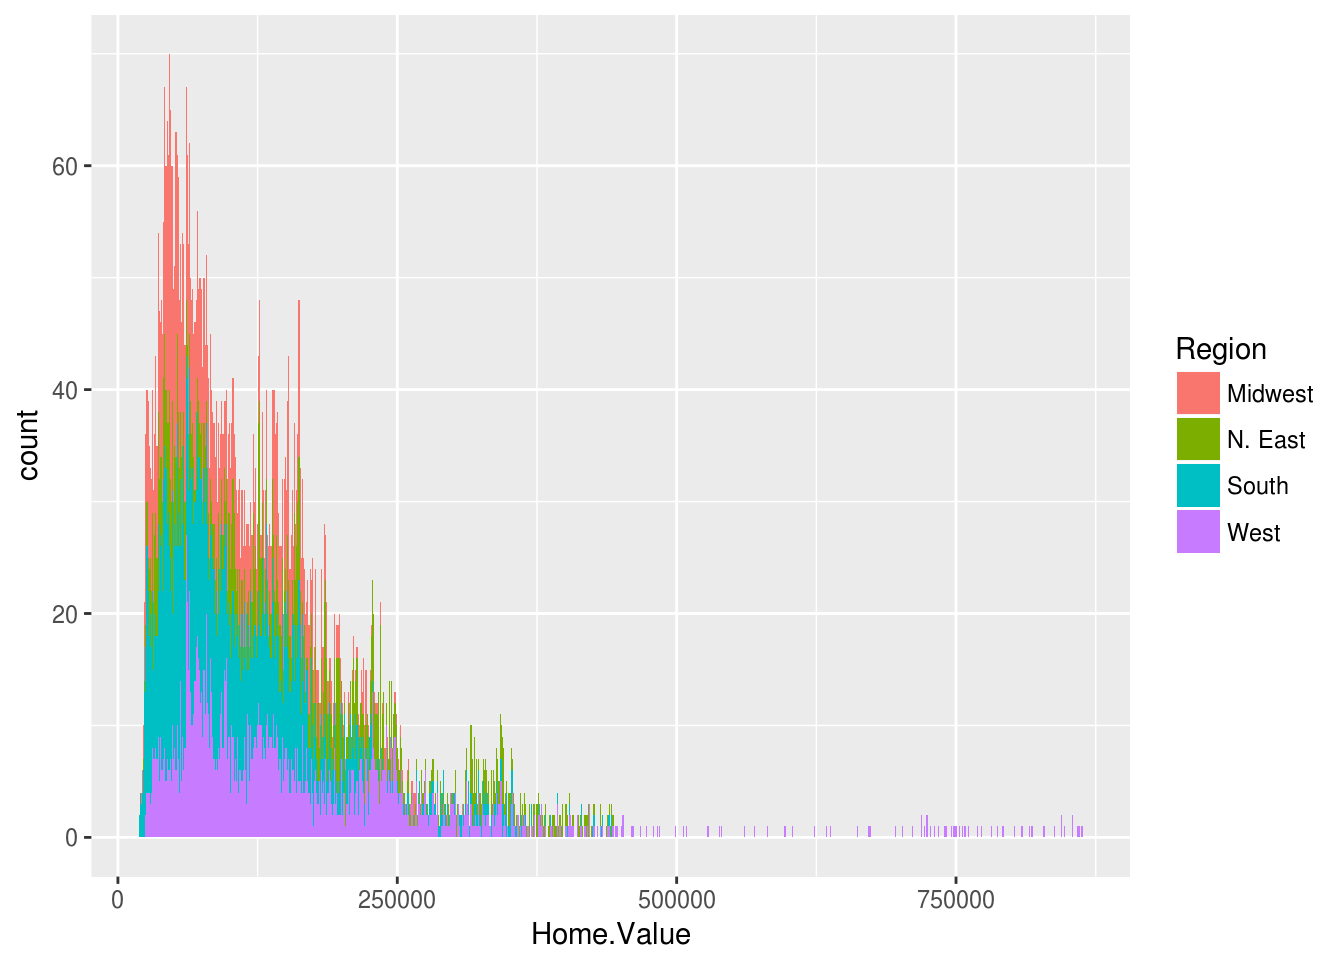
\includegraphics{ggplot_tutorial_files/figure-latex/unnamed-chunk-17-1.pdf}

Mapping can also be specified in the geom:

\begin{Shaded}
\begin{Highlighting}[]
\KeywordTok{ggplot}\NormalTok{(housing, }\KeywordTok{aes}\NormalTok{(}\DataTypeTok{x =} \NormalTok{Home.Value)) +}
\StringTok{  }\KeywordTok{geom_histogram}\NormalTok{(}\KeywordTok{aes}\NormalTok{(}\DataTypeTok{fill =} \NormalTok{Region), }\DataTypeTok{binwidth =} \DecValTok{1000}\NormalTok{)}
\end{Highlighting}
\end{Shaded}

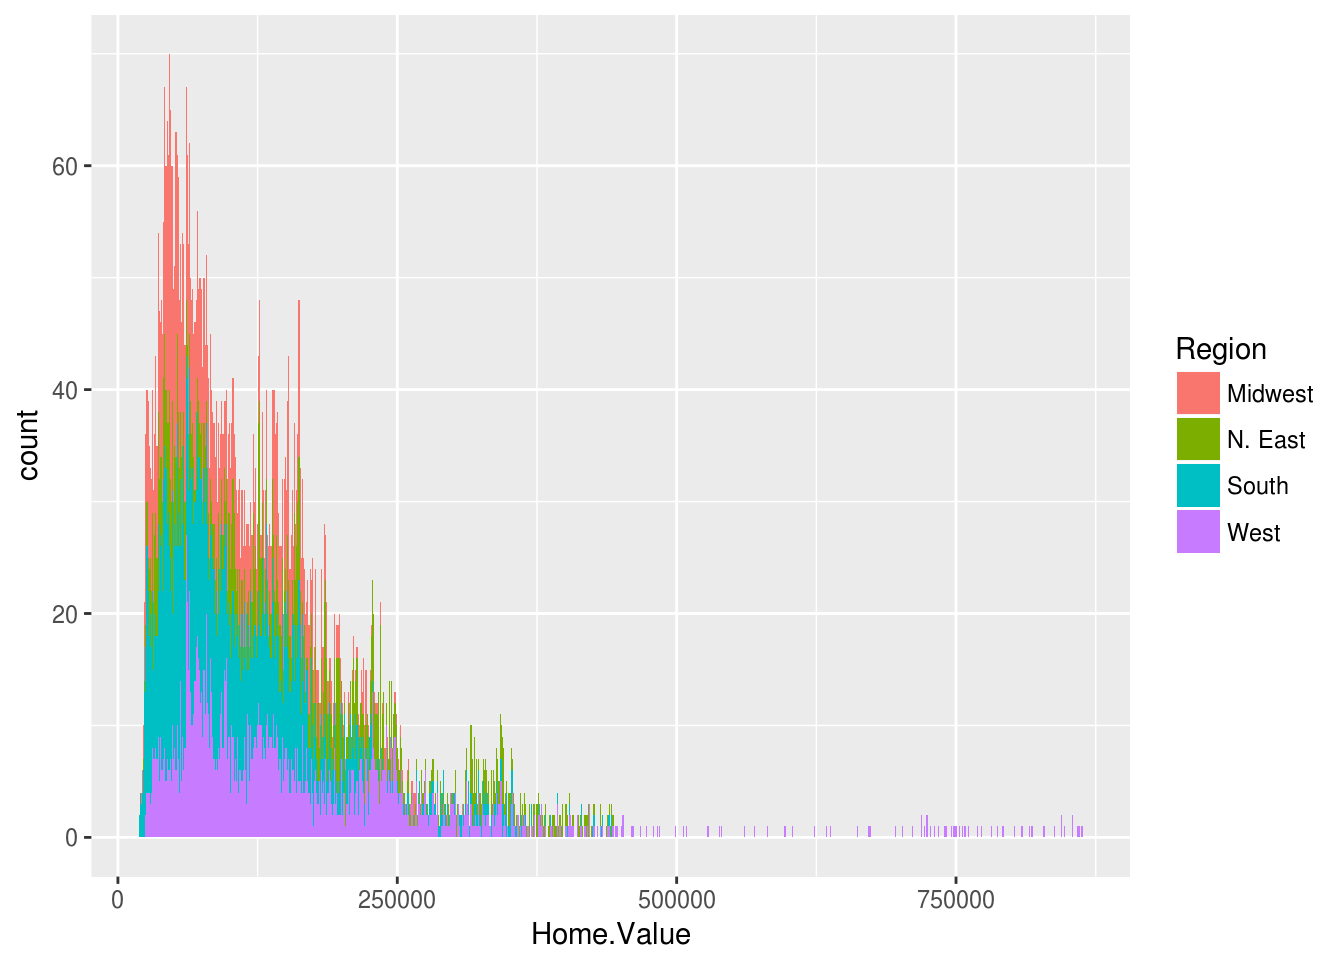
\includegraphics{ggplot_tutorial_files/figure-latex/unnamed-chunk-18-1.pdf}

Same plot can also be created using \texttt{stat\_bin} transformation.
The default geom for stat\_bin is ``area''

\begin{Shaded}
\begin{Highlighting}[]
\KeywordTok{ggplot}\NormalTok{(housing, }\KeywordTok{aes}\NormalTok{(}\DataTypeTok{x =} \NormalTok{Home.Value)) +}
\StringTok{  }\KeywordTok{stat_bin}\NormalTok{(}\DataTypeTok{binwidth =} \DecValTok{1000}\NormalTok{)}
\end{Highlighting}
\end{Shaded}

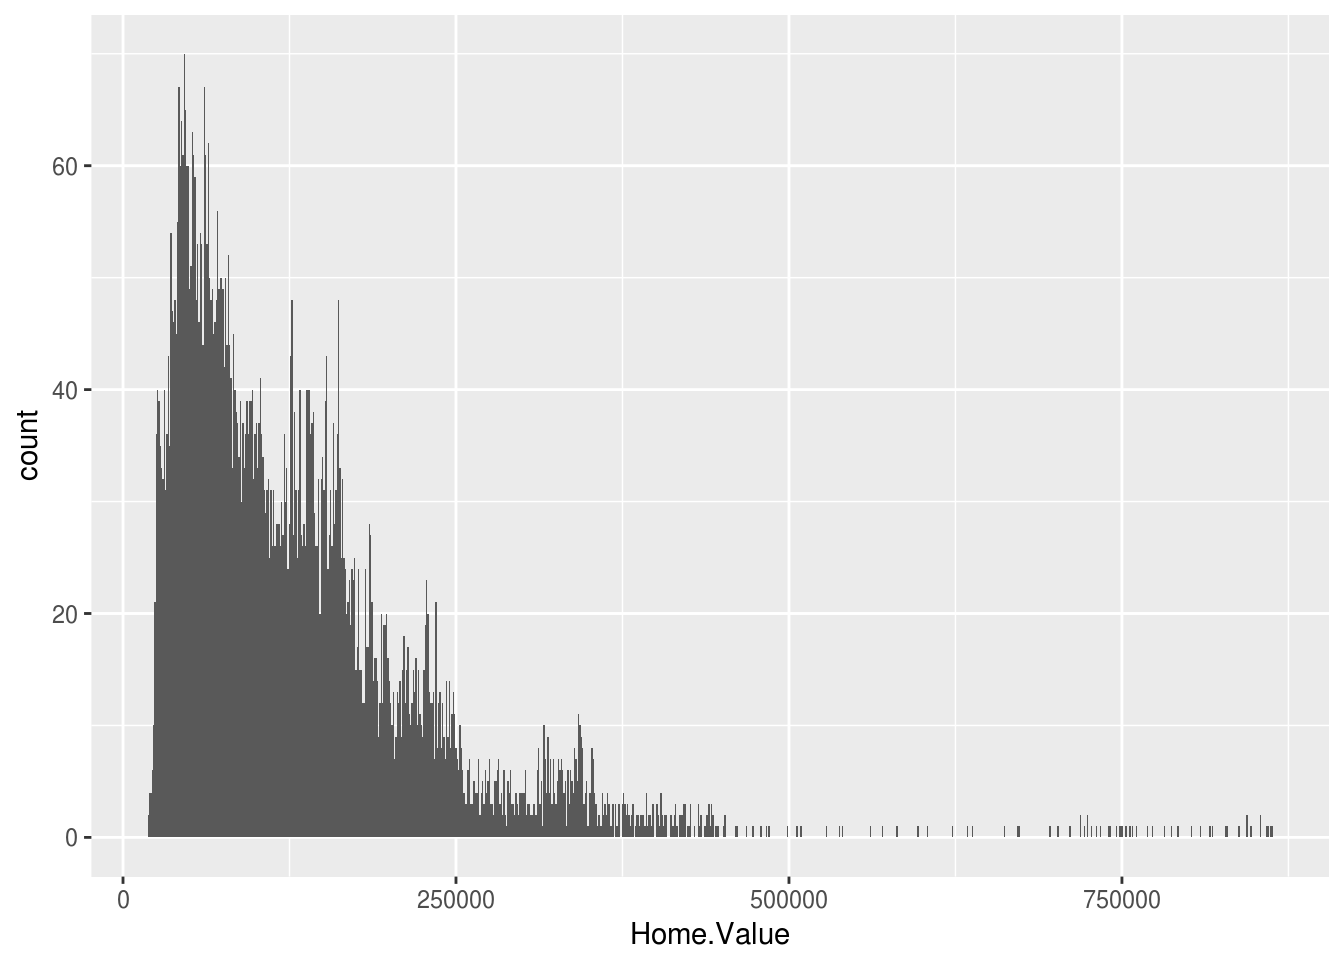
\includegraphics{ggplot_tutorial_files/figure-latex/unnamed-chunk-19-1.pdf}

Change the default geom to \texttt{"point"}

\begin{Shaded}
\begin{Highlighting}[]
\KeywordTok{ggplot}\NormalTok{(housing, }\KeywordTok{aes}\NormalTok{(}\DataTypeTok{x =} \NormalTok{Home.Value)) +}
\StringTok{  }\KeywordTok{stat_bin}\NormalTok{(}\DataTypeTok{geom =} \StringTok{"point"}\NormalTok{, }\DataTypeTok{binwidth =} \DecValTok{1000}\NormalTok{)}
\end{Highlighting}
\end{Shaded}

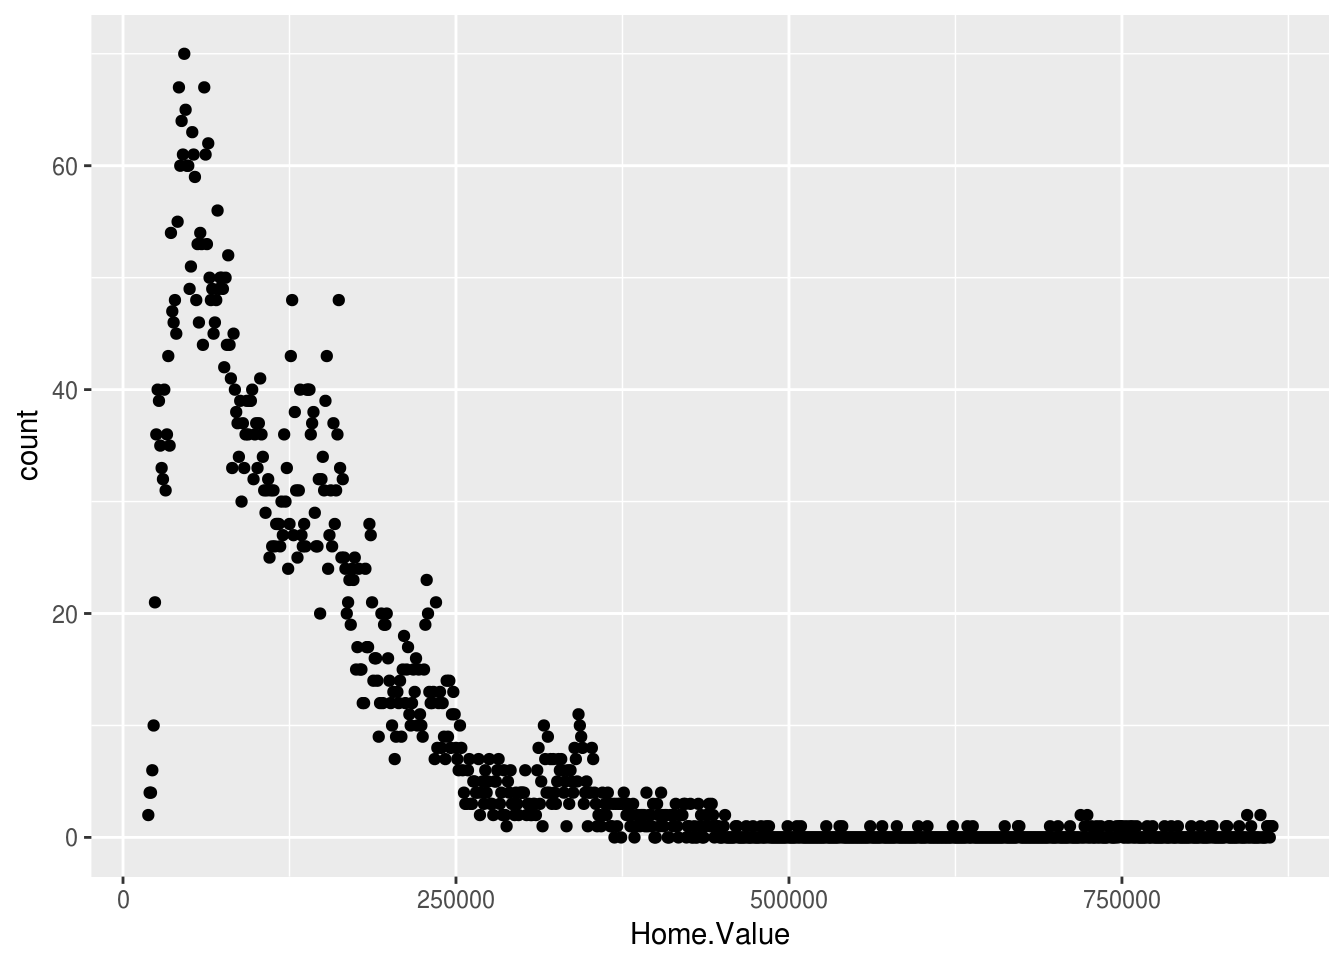
\includegraphics{ggplot_tutorial_files/figure-latex/unnamed-chunk-20-1.pdf}

Change the default geom to \texttt{"line"}

\begin{Shaded}
\begin{Highlighting}[]
\KeywordTok{ggplot}\NormalTok{(housing, }\KeywordTok{aes}\NormalTok{(}\DataTypeTok{x =} \NormalTok{Home.Value)) +}
\StringTok{  }\KeywordTok{stat_bin}\NormalTok{(}\DataTypeTok{geom =} \StringTok{"line"}\NormalTok{, }\DataTypeTok{binwidth =} \DecValTok{1000}\NormalTok{)}
\end{Highlighting}
\end{Shaded}

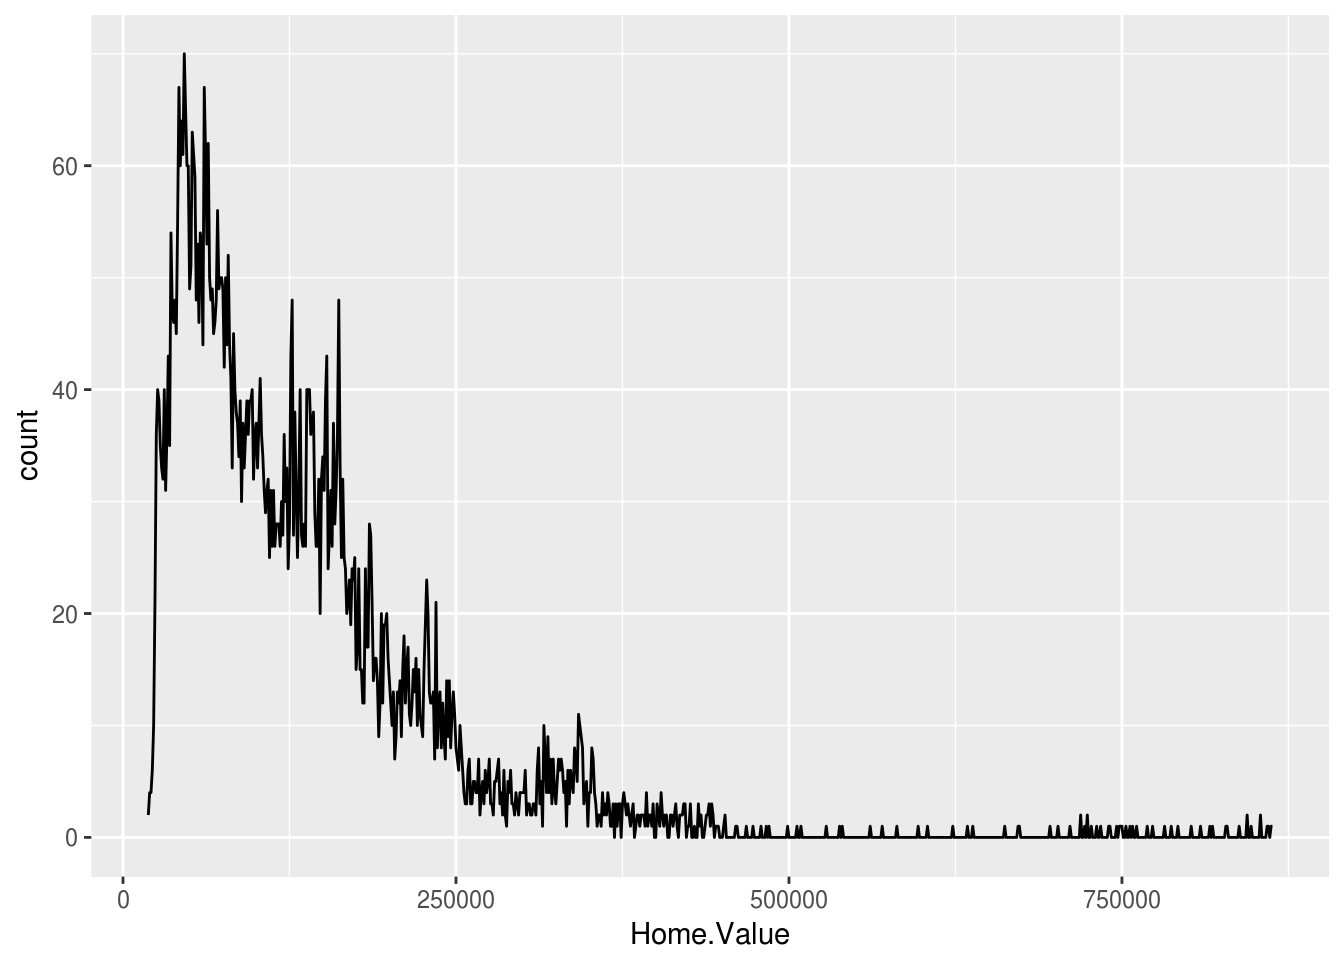
\includegraphics{ggplot_tutorial_files/figure-latex/unnamed-chunk-21-1.pdf}

\subsection{Exercise}\label{exercise-1}

Create a subset of housing data from New York since 2000

\begin{Shaded}
\begin{Highlighting}[]
\NormalTok{newyork2k <-}\StringTok{ }\KeywordTok{subset}\NormalTok{(newyork, Year >=}\StringTok{ }\DecValTok{2000}\NormalTok{)}
\end{Highlighting}
\end{Shaded}

\begin{enumerate}
\def\labelenumi{\arabic{enumi}.}
\item
  Create a plot that includes multiple geometric objects, for example,
  lines and points.

  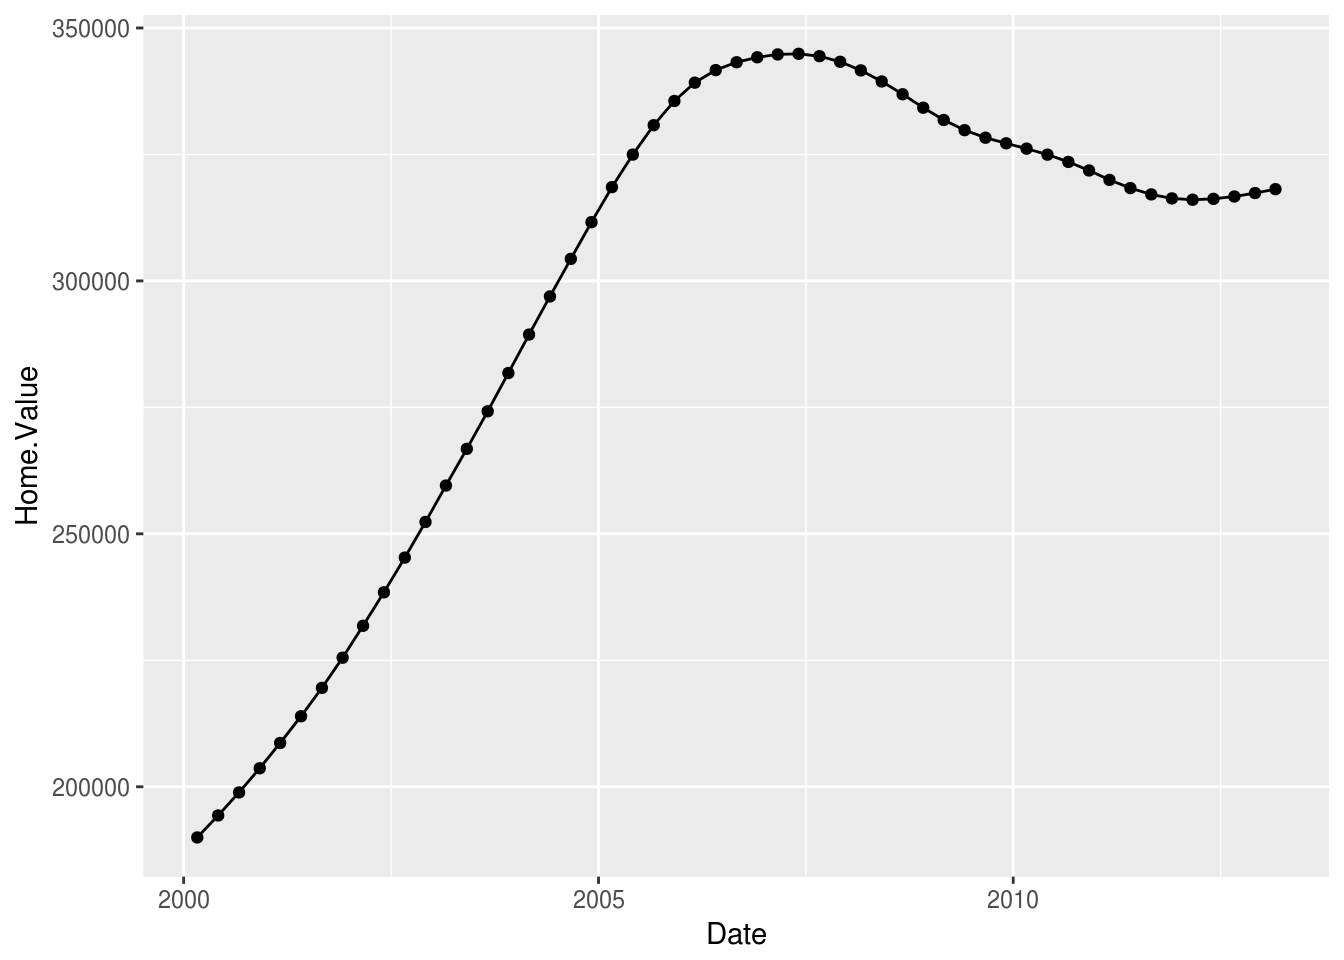
\includegraphics{ggplot_tutorial_files/figure-latex/unnamed-chunk-23-1.pdf}
\item
  Change the shape to be hollow diamond

  HINT: Take a look at \textbf{Shape Scales} in the
  \href{https://www.rstudio.com/wp-content/uploads/2015/03/ggplot2-cheatsheet.pdf}{Data
  Visualization with ggplot2 Cheat Sheet}

  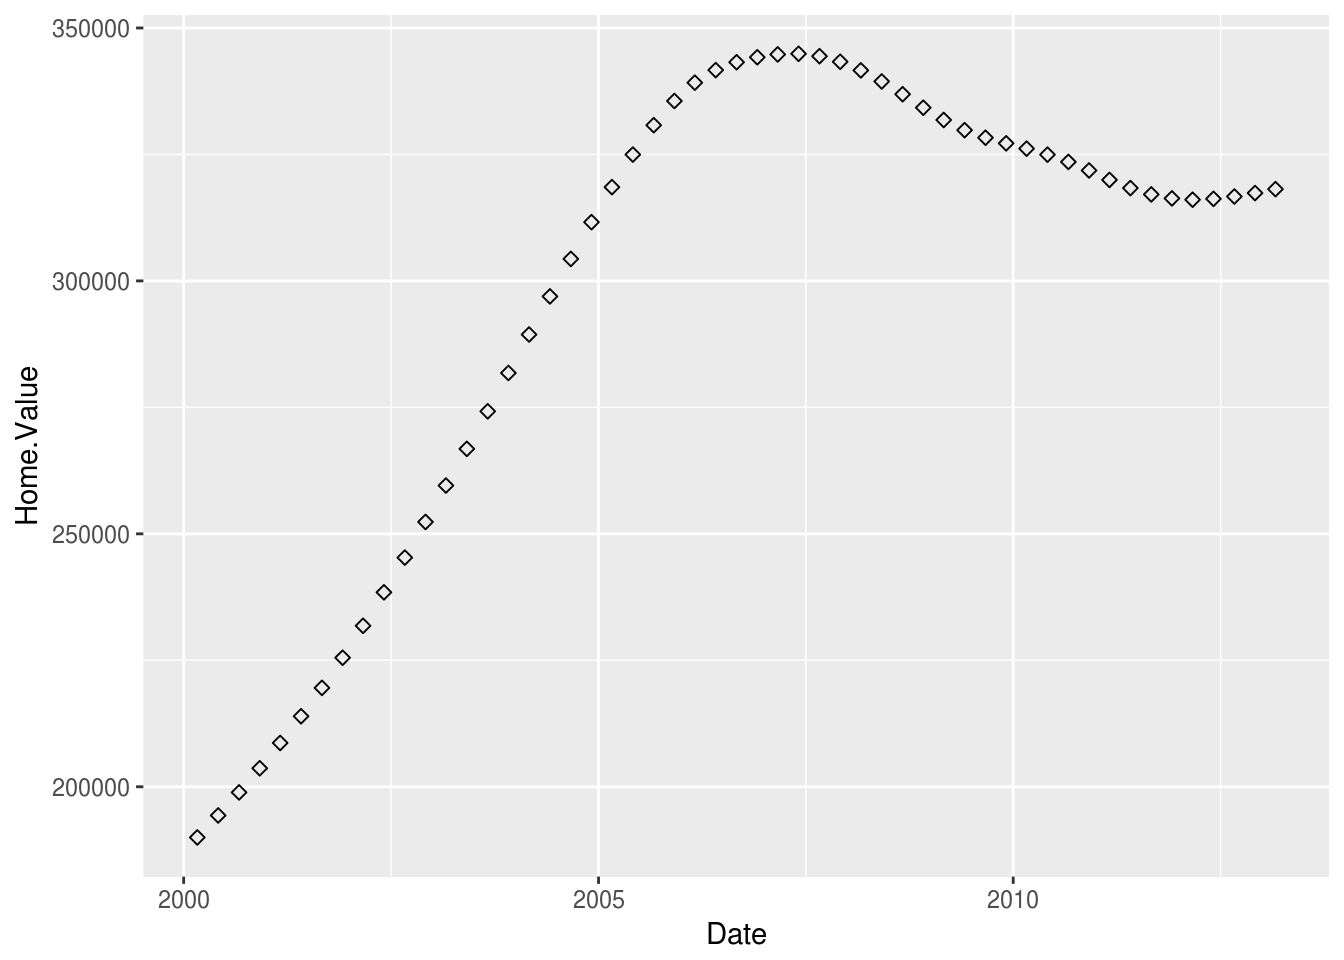
\includegraphics{ggplot_tutorial_files/figure-latex/unnamed-chunk-24-1.pdf}
\item
  Change the size of the point based on \texttt{Land.Value} and color
  based on \texttt{Structure.Cost}

  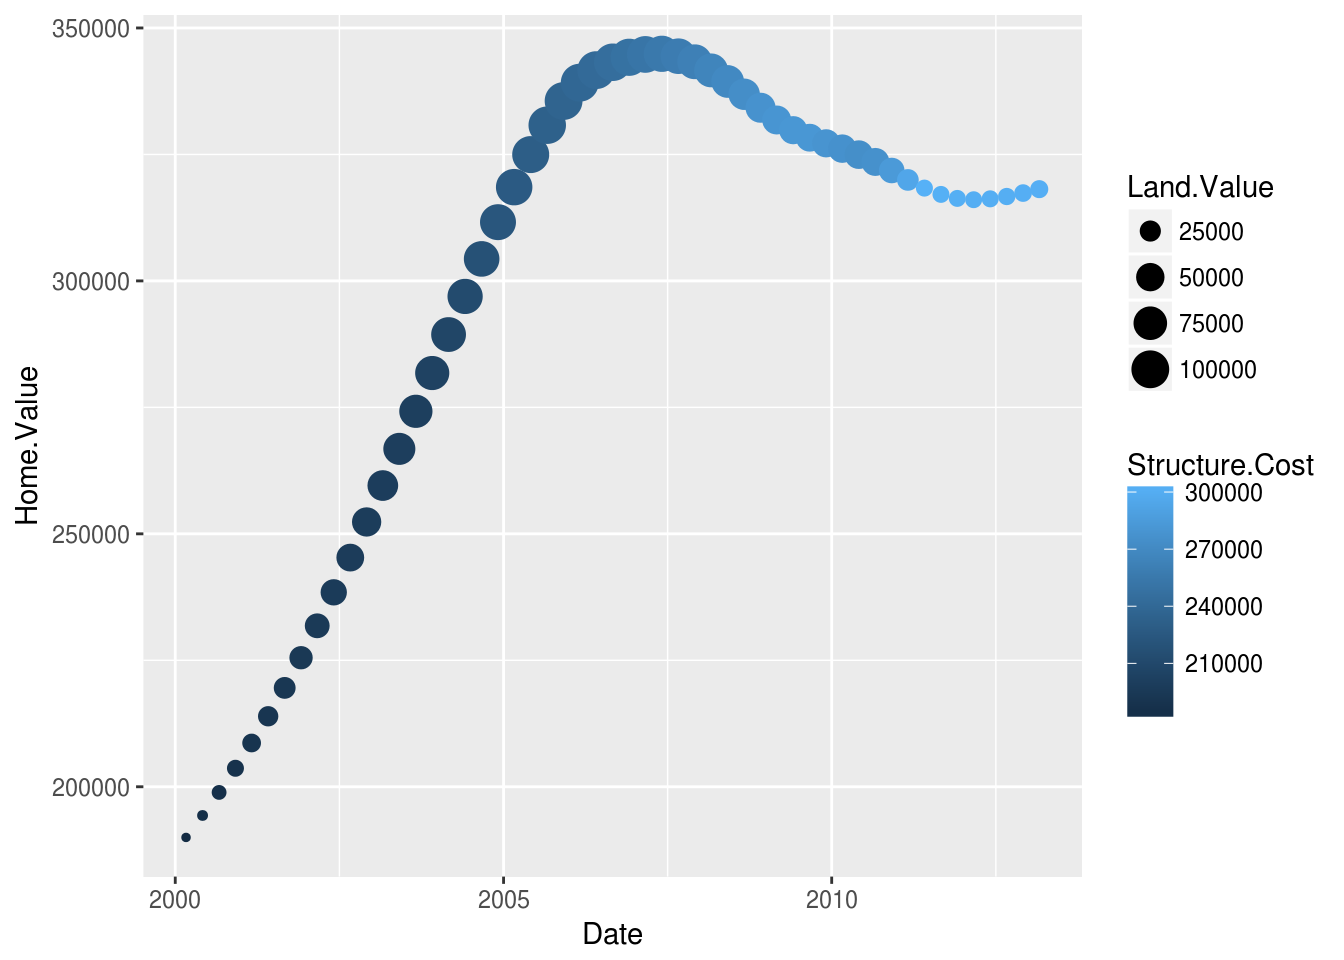
\includegraphics{ggplot_tutorial_files/figure-latex/unnamed-chunk-25-1.pdf}
\end{enumerate}

\section{Scales}\label{scales}

Let's create another subset that includes only the data from the first
quarter of 2001.

\begin{Shaded}
\begin{Highlighting}[]
\NormalTok{housing2001q1 <-}\StringTok{ }\KeywordTok{subset}\NormalTok{(housing, Year ==}\StringTok{ }\DecValTok{2001} \NormalTok{&}\StringTok{ }\NormalTok{Quarter ==}\StringTok{ }\DecValTok{1}\NormalTok{)}
\end{Highlighting}
\end{Shaded}

And now we create a scatter plot with this dataset

\begin{Shaded}
\begin{Highlighting}[]
\KeywordTok{ggplot}\NormalTok{(housing2001q1, }\KeywordTok{aes}\NormalTok{(}\DataTypeTok{x =} \NormalTok{Land.Value, }\DataTypeTok{y =} \NormalTok{Structure.Cost)) +}\StringTok{ }
\StringTok{  }\KeywordTok{geom_point}\NormalTok{()}
\end{Highlighting}
\end{Shaded}

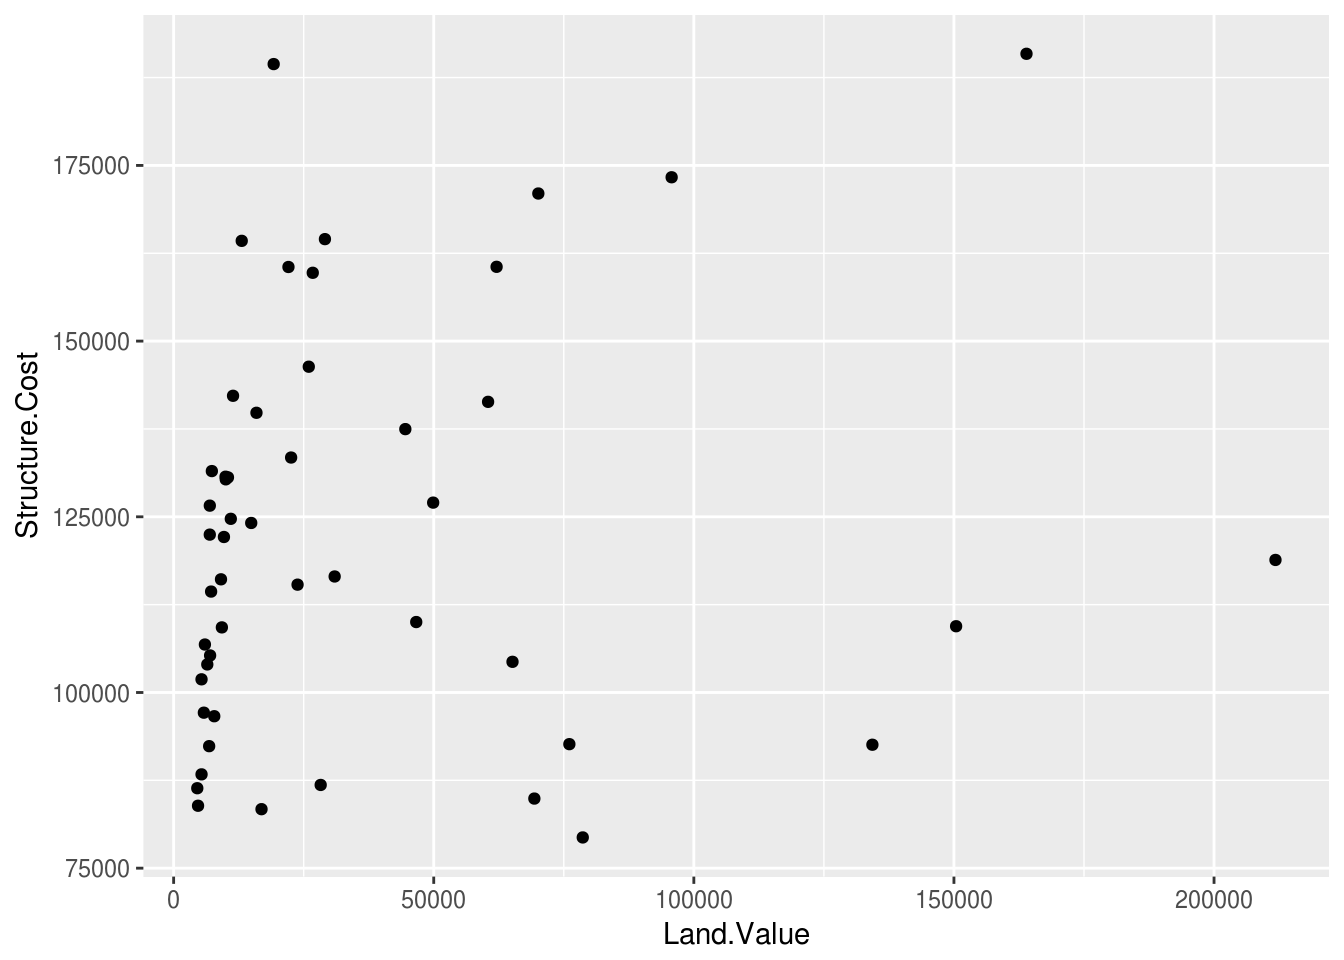
\includegraphics{ggplot_tutorial_files/figure-latex/unnamed-chunk-27-1.pdf}

Our dataset is skewed so in order to help with interpretation, let's
change the x-axis to log scale

\begin{Shaded}
\begin{Highlighting}[]
\KeywordTok{ggplot}\NormalTok{(housing2001q1, }\KeywordTok{aes}\NormalTok{(}\DataTypeTok{x =} \NormalTok{Land.Value, }\DataTypeTok{y =} \NormalTok{Structure.Cost)) +}\StringTok{ }
\StringTok{  }\KeywordTok{geom_point}\NormalTok{() +}\StringTok{ }
\StringTok{  }\KeywordTok{scale_x_log10}\NormalTok{()}
\end{Highlighting}
\end{Shaded}

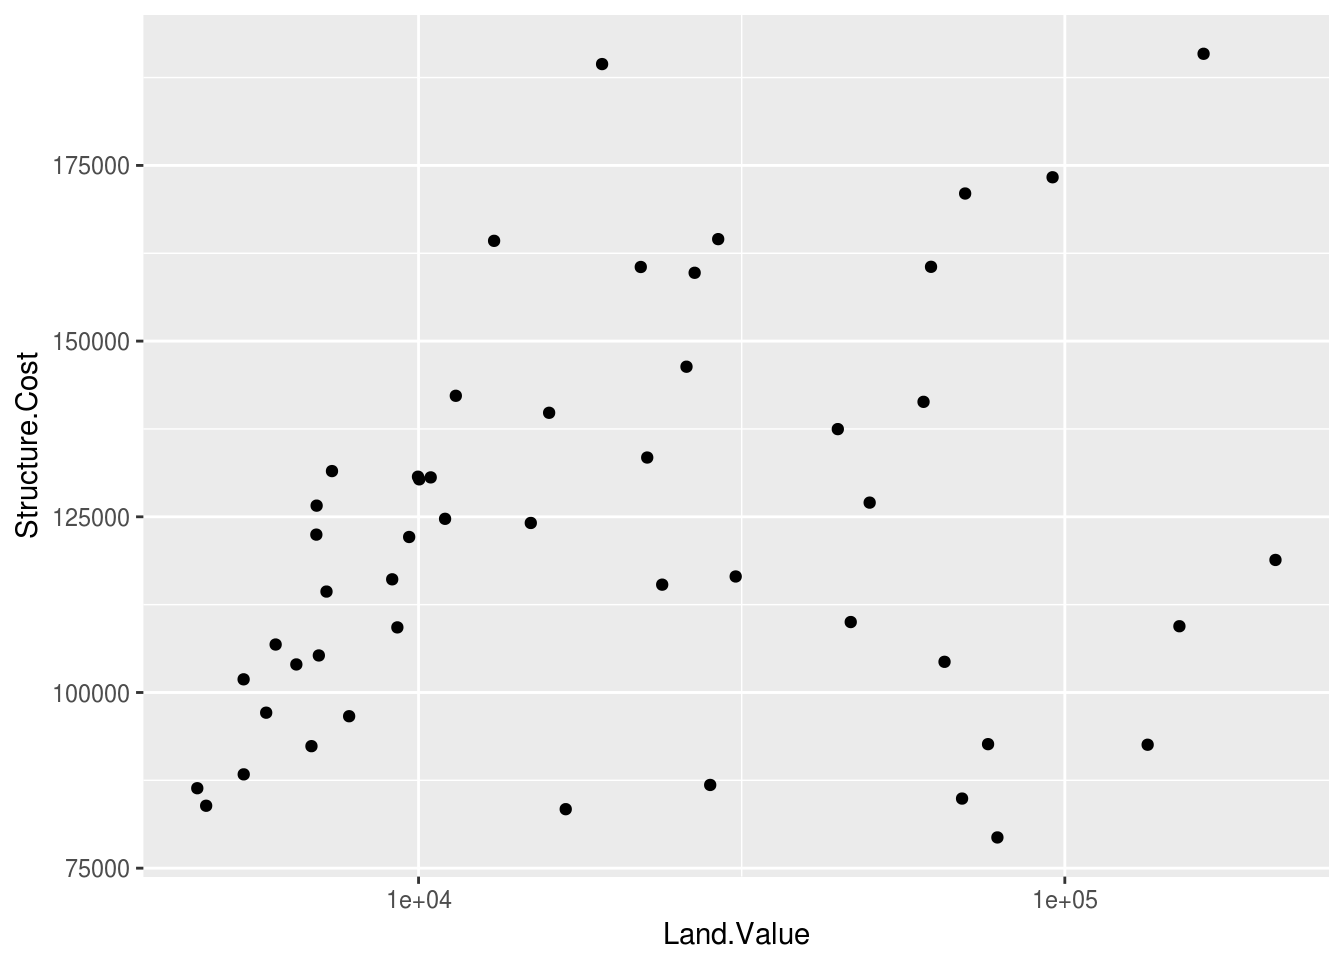
\includegraphics{ggplot_tutorial_files/figure-latex/unnamed-chunk-28-1.pdf}

Now add a dollar sign in front of our axis labels

\begin{Shaded}
\begin{Highlighting}[]
\KeywordTok{ggplot}\NormalTok{(housing2001q1, }\KeywordTok{aes}\NormalTok{(}\DataTypeTok{x =} \NormalTok{Land.Value, }\DataTypeTok{y =} \NormalTok{Structure.Cost)) +}\StringTok{ }
\StringTok{  }\KeywordTok{geom_point}\NormalTok{() +}\StringTok{ }
\StringTok{  }\KeywordTok{scale_x_log10}\NormalTok{(}\DataTypeTok{labels =} \NormalTok{dollar) +}
\StringTok{  }\KeywordTok{scale_y_continuous}\NormalTok{(}\DataTypeTok{labels =} \NormalTok{dollar)}
\end{Highlighting}
\end{Shaded}

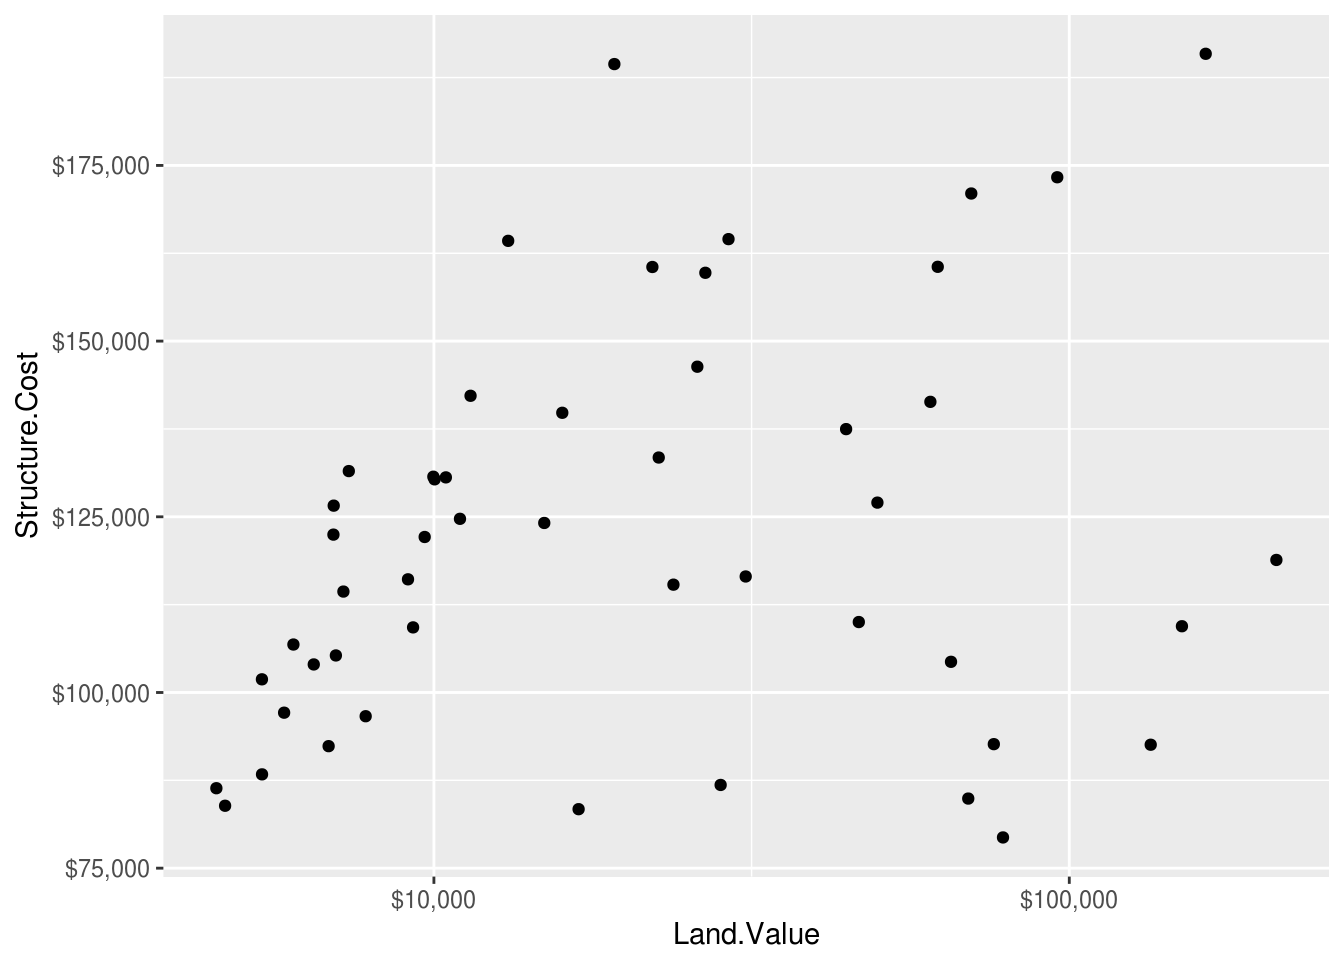
\includegraphics{ggplot_tutorial_files/figure-latex/unnamed-chunk-29-1.pdf}

Next we change the scale for the x-axis which is in a Date format and
control the breaks for y-axis which is a continuous variable.

\begin{Shaded}
\begin{Highlighting}[]
\KeywordTok{ggplot}\NormalTok{(northeast, }\KeywordTok{aes}\NormalTok{(}\DataTypeTok{x =} \NormalTok{Date, }\DataTypeTok{y =} \NormalTok{Home.Value, }\DataTypeTok{color =} \NormalTok{State)) +}
\StringTok{  }\KeywordTok{geom_line}\NormalTok{() +}
\StringTok{  }\KeywordTok{scale_x_date}\NormalTok{(}\DataTypeTok{date_breaks =}\StringTok{"3 year"}\NormalTok{, }\DataTypeTok{date_minor_breaks =}\StringTok{"1 year"}\NormalTok{, }\DataTypeTok{date_labels =} \StringTok{"'%y"}\NormalTok{) +}
\StringTok{  }\KeywordTok{scale_y_continuous}\NormalTok{(}\DataTypeTok{breaks =} \KeywordTok{seq}\NormalTok{(}\DecValTok{0}\NormalTok{, }\DecValTok{500000}\NormalTok{, }\DecValTok{50000}\NormalTok{), }\DataTypeTok{labels =} \NormalTok{dollar) }
\end{Highlighting}
\end{Shaded}

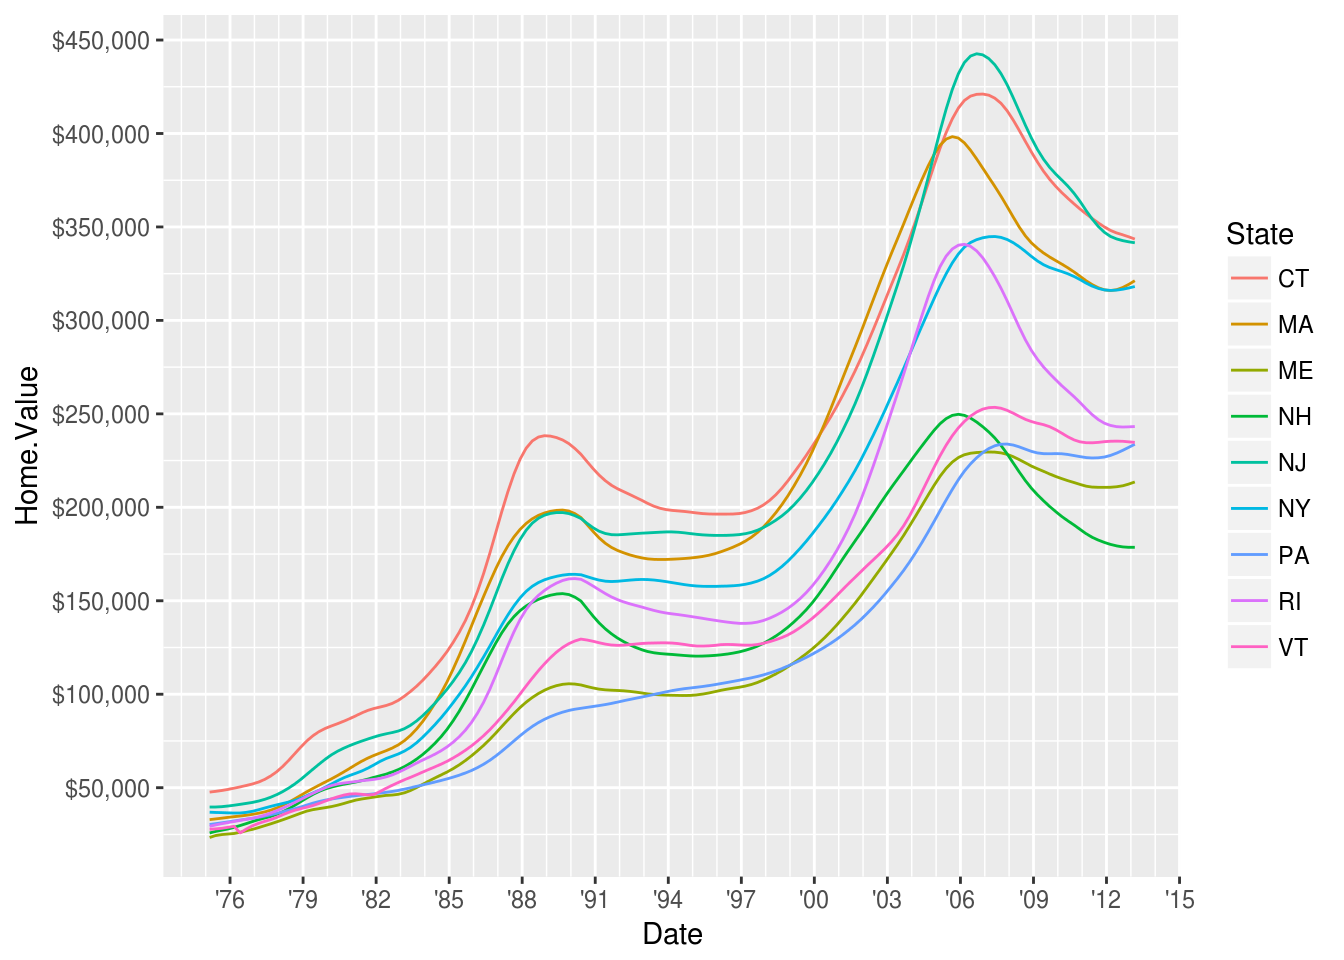
\includegraphics{ggplot_tutorial_files/figure-latex/unnamed-chunk-30-1.pdf}

\section{Text and Labels}\label{text-and-labels}

Let's continue with the subset of the data from the previous section and
add text to the scatterplot.

\begin{Shaded}
\begin{Highlighting}[]
\KeywordTok{ggplot}\NormalTok{(housing2001q1, }\KeywordTok{aes}\NormalTok{(}\DataTypeTok{x =} \NormalTok{Land.Value, }\DataTypeTok{y =} \NormalTok{Structure.Cost)) +}\StringTok{ }
\StringTok{  }\KeywordTok{geom_point}\NormalTok{() +}
\StringTok{  }\KeywordTok{geom_text}\NormalTok{(}\KeywordTok{aes}\NormalTok{(}\DataTypeTok{label =} \NormalTok{State))}
\end{Highlighting}
\end{Shaded}

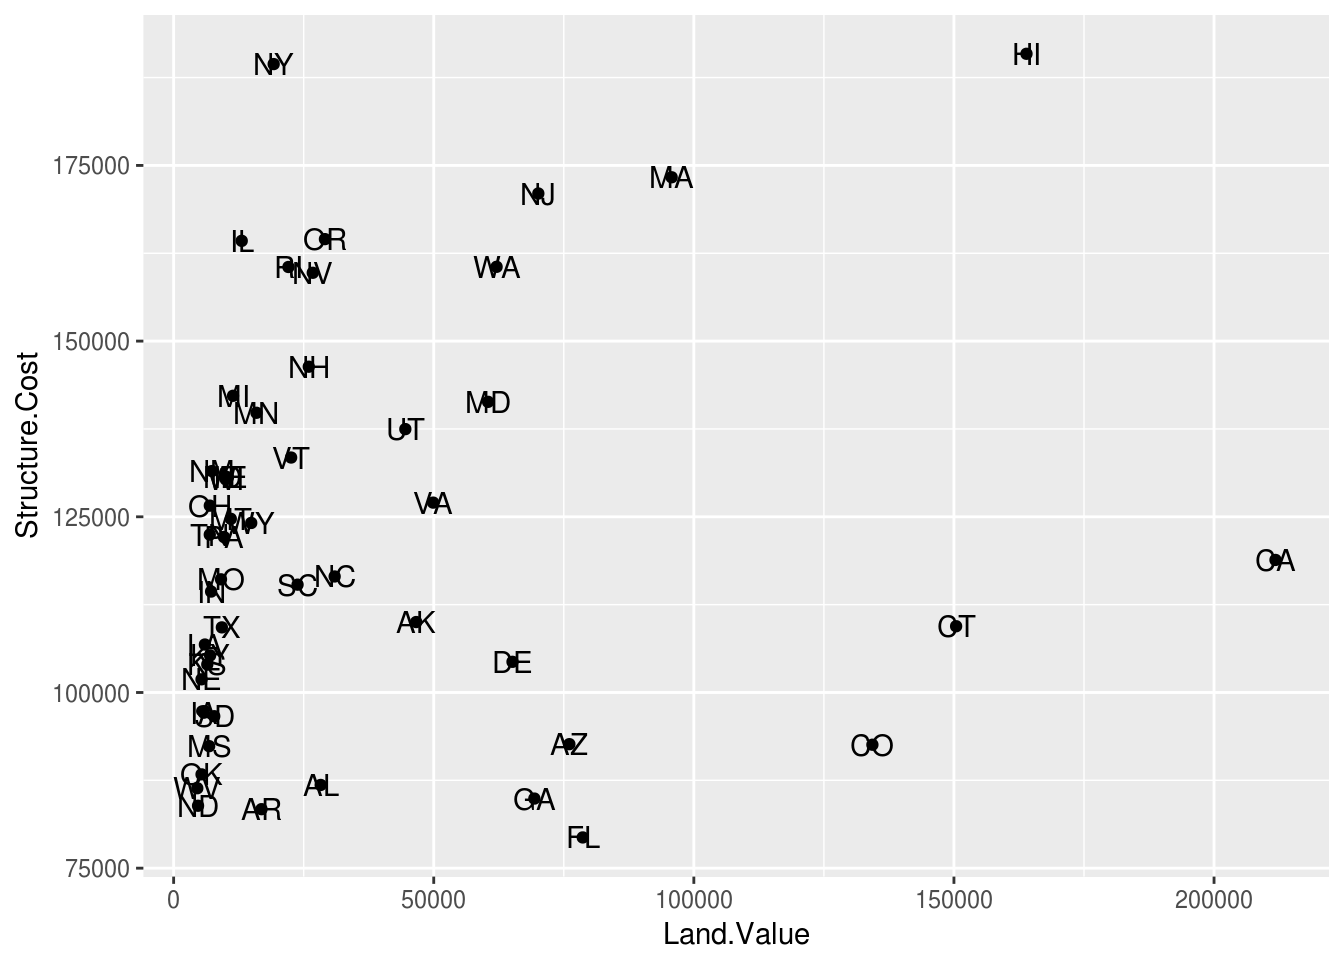
\includegraphics{ggplot_tutorial_files/figure-latex/unnamed-chunk-31-1.pdf}

The result isn't very nice as the labels overlap each other. Let's try
the same with \texttt{geom\_label()} instead which draws the text with a
border around it.

\begin{Shaded}
\begin{Highlighting}[]
\KeywordTok{ggplot}\NormalTok{(housing2001q1, }\KeywordTok{aes}\NormalTok{(}\DataTypeTok{x =} \NormalTok{Land.Value, }\DataTypeTok{y =} \NormalTok{Structure.Cost)) +}\StringTok{ }
\StringTok{  }\KeywordTok{geom_point}\NormalTok{() +}
\StringTok{  }\KeywordTok{geom_label}\NormalTok{(}\KeywordTok{aes}\NormalTok{(}\DataTypeTok{label =} \NormalTok{State))}
\end{Highlighting}
\end{Shaded}

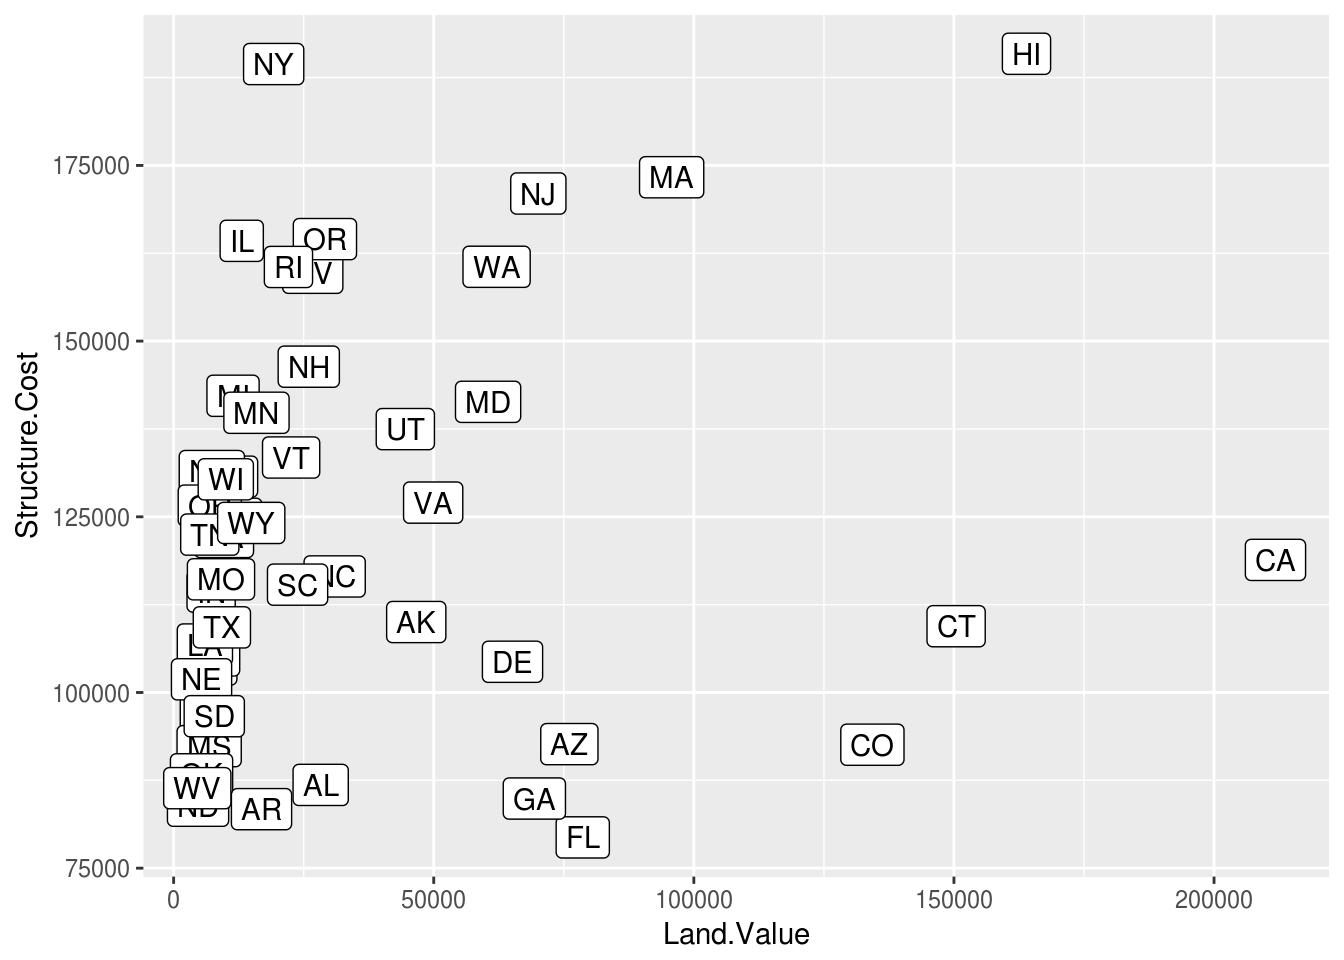
\includegraphics{ggplot_tutorial_files/figure-latex/unnamed-chunk-32-1.pdf}

The \texttt{ggrepel} extension we loaded earlier can also help fix this
problem.

\begin{Shaded}
\begin{Highlighting}[]
\KeywordTok{ggplot}\NormalTok{(housing2001q1, }\KeywordTok{aes}\NormalTok{(}\DataTypeTok{x =} \NormalTok{Land.Value, }\DataTypeTok{y =} \NormalTok{Structure.Cost)) +}\StringTok{ }
\StringTok{  }\KeywordTok{geom_point}\NormalTok{() +}
\StringTok{  }\KeywordTok{geom_text_repel}\NormalTok{(}\KeywordTok{aes}\NormalTok{(}\DataTypeTok{label =} \NormalTok{State))}
\end{Highlighting}
\end{Shaded}

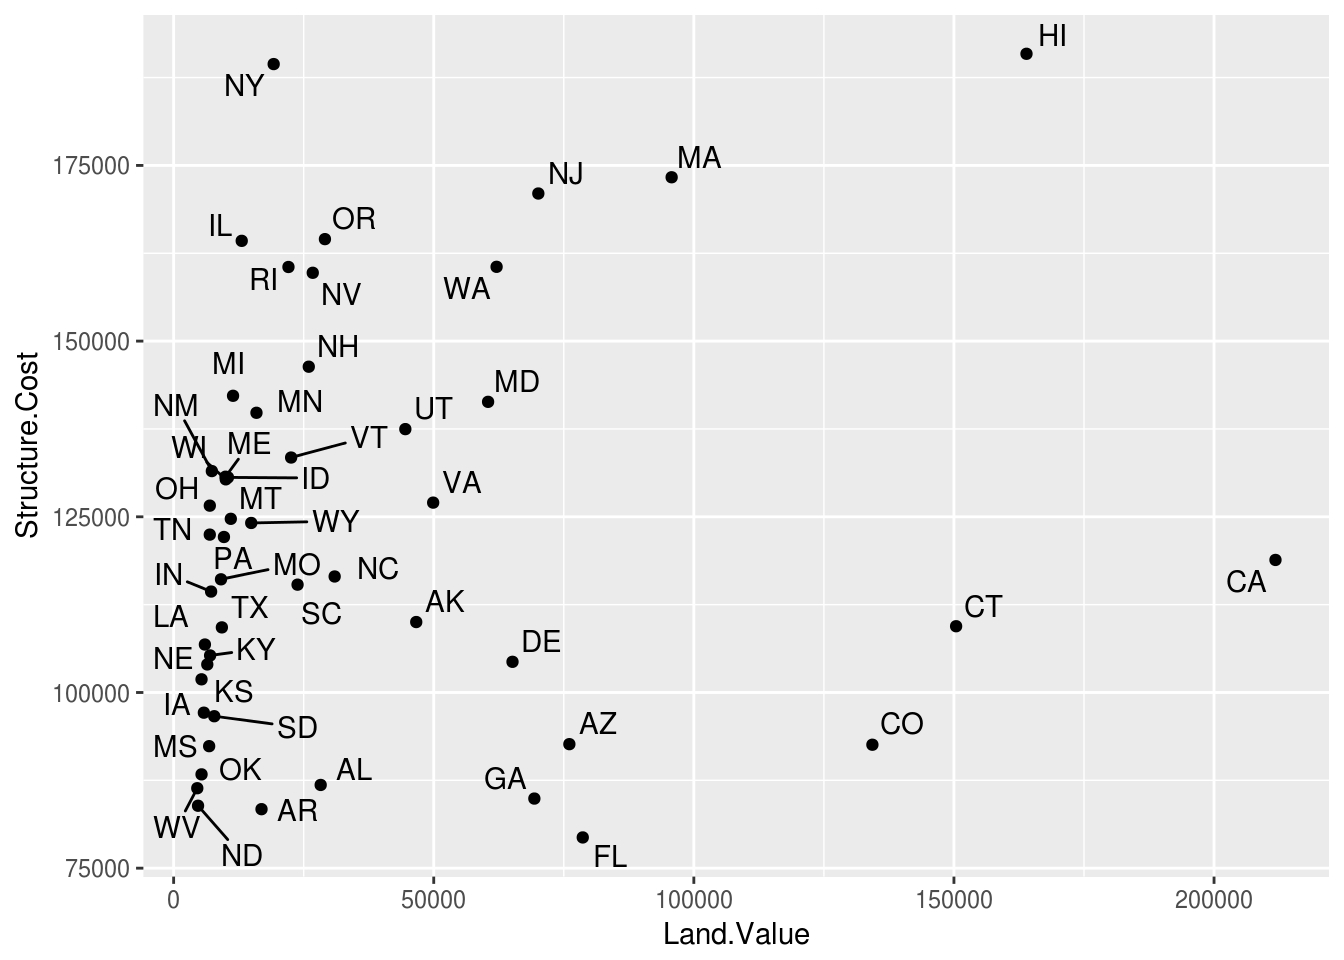
\includegraphics{ggplot_tutorial_files/figure-latex/unnamed-chunk-33-1.pdf}

And we can repel the labels with a border using
\texttt{geom\_label\_repel()}.

\begin{Shaded}
\begin{Highlighting}[]
\KeywordTok{ggplot}\NormalTok{(housing2001q1, }\KeywordTok{aes}\NormalTok{(}\DataTypeTok{x =} \NormalTok{Land.Value, }\DataTypeTok{y =} \NormalTok{Structure.Cost)) +}\StringTok{ }
\StringTok{  }\KeywordTok{geom_point}\NormalTok{() +}
\StringTok{  }\KeywordTok{geom_label_repel}\NormalTok{(}\KeywordTok{aes}\NormalTok{(}\DataTypeTok{label =} \NormalTok{State))}
\end{Highlighting}
\end{Shaded}

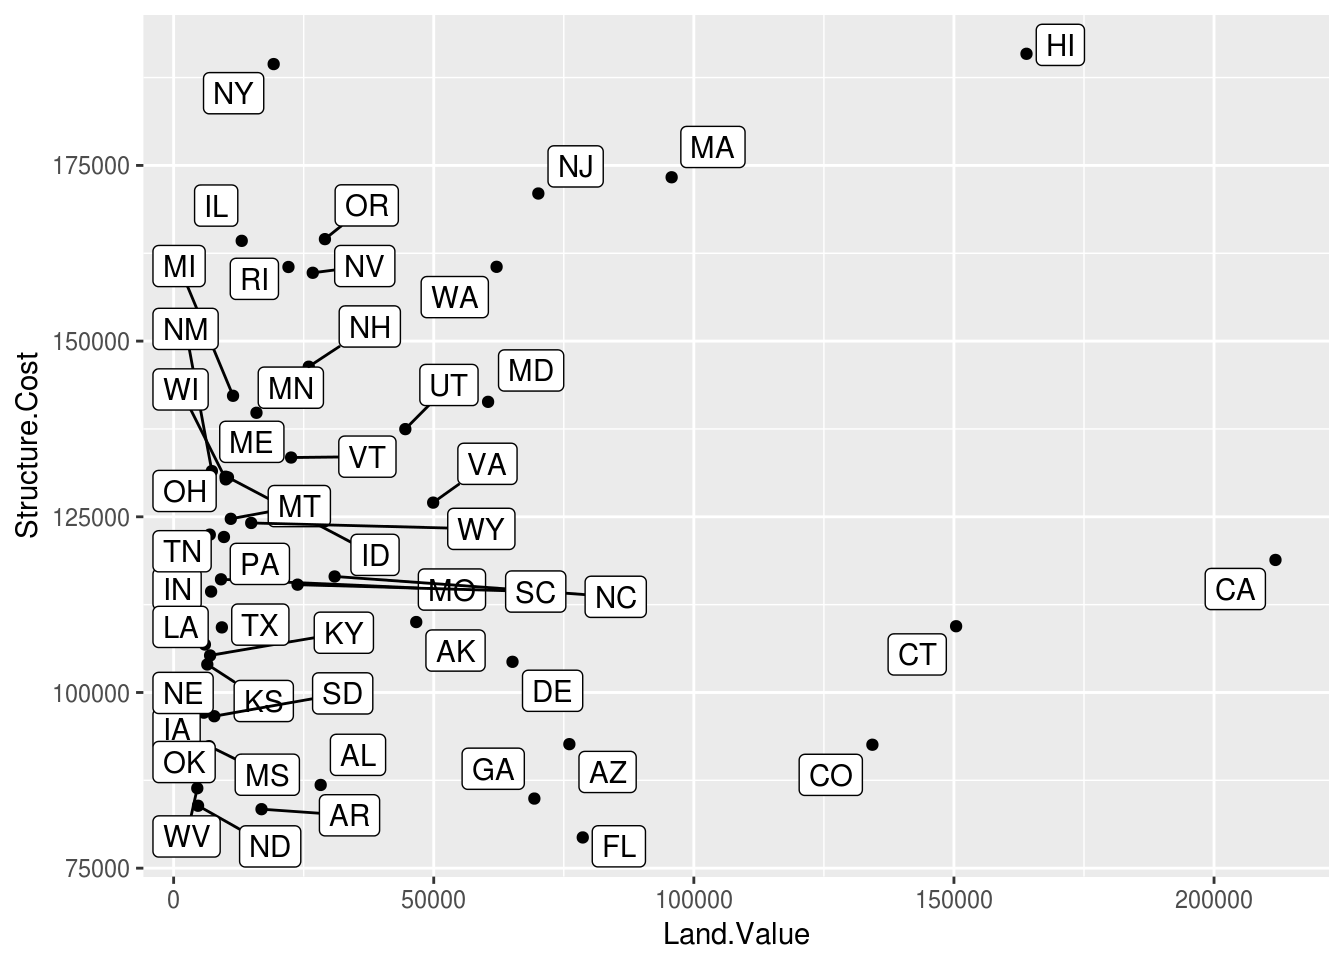
\includegraphics{ggplot_tutorial_files/figure-latex/unnamed-chunk-34-1.pdf}

\section{Smoother}\label{smoother}

Let's continue with the 2001 first quarter dataset and add a smoother.

\begin{Shaded}
\begin{Highlighting}[]
\KeywordTok{ggplot}\NormalTok{(housing2001q1, }\KeywordTok{aes}\NormalTok{(}\DataTypeTok{x =} \NormalTok{Land.Value, }\DataTypeTok{y =} \NormalTok{Structure.Cost)) +}\StringTok{ }
\StringTok{  }\KeywordTok{geom_point}\NormalTok{() +}\StringTok{ }
\StringTok{  }\KeywordTok{scale_x_log10}\NormalTok{() +}
\StringTok{  }\KeywordTok{stat_smooth}\NormalTok{()}
\end{Highlighting}
\end{Shaded}

\begin{verbatim}
## `geom_smooth()` using method = 'loess'
\end{verbatim}

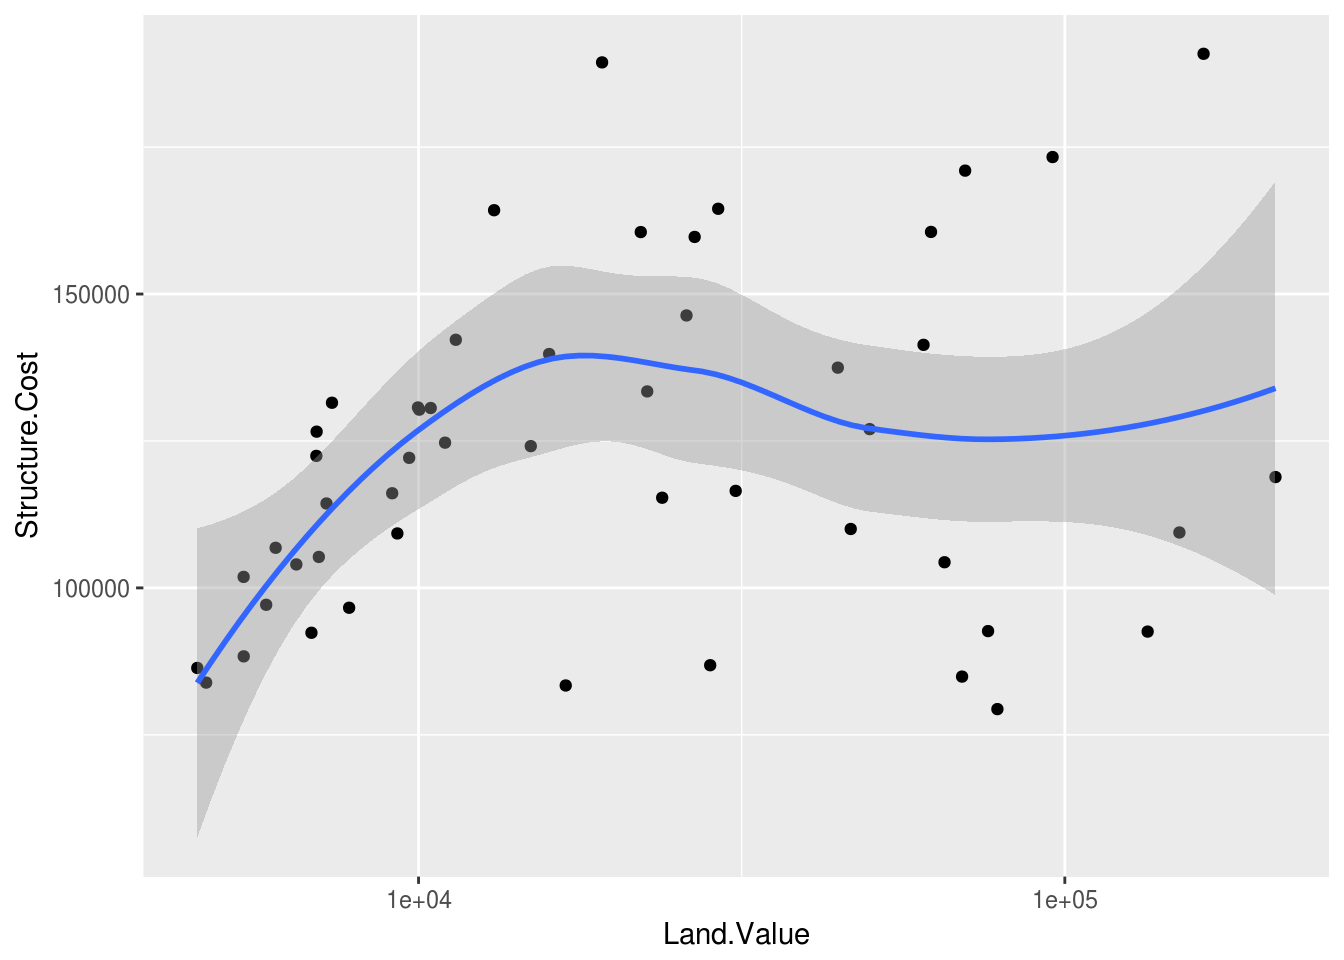
\includegraphics{ggplot_tutorial_files/figure-latex/unnamed-chunk-35-1.pdf}

We can fit a linear model to our dataset

\begin{Shaded}
\begin{Highlighting}[]
\KeywordTok{ggplot}\NormalTok{(housing2001q1, }\KeywordTok{aes}\NormalTok{(}\DataTypeTok{x =} \NormalTok{Land.Value, }\DataTypeTok{y =} \NormalTok{Structure.Cost)) +}\StringTok{ }
\StringTok{  }\KeywordTok{geom_point}\NormalTok{() +}
\StringTok{  }\KeywordTok{scale_x_log10}\NormalTok{() +}
\StringTok{  }\KeywordTok{stat_smooth}\NormalTok{(}\DataTypeTok{method =} \StringTok{"lm"}\NormalTok{)}
\end{Highlighting}
\end{Shaded}

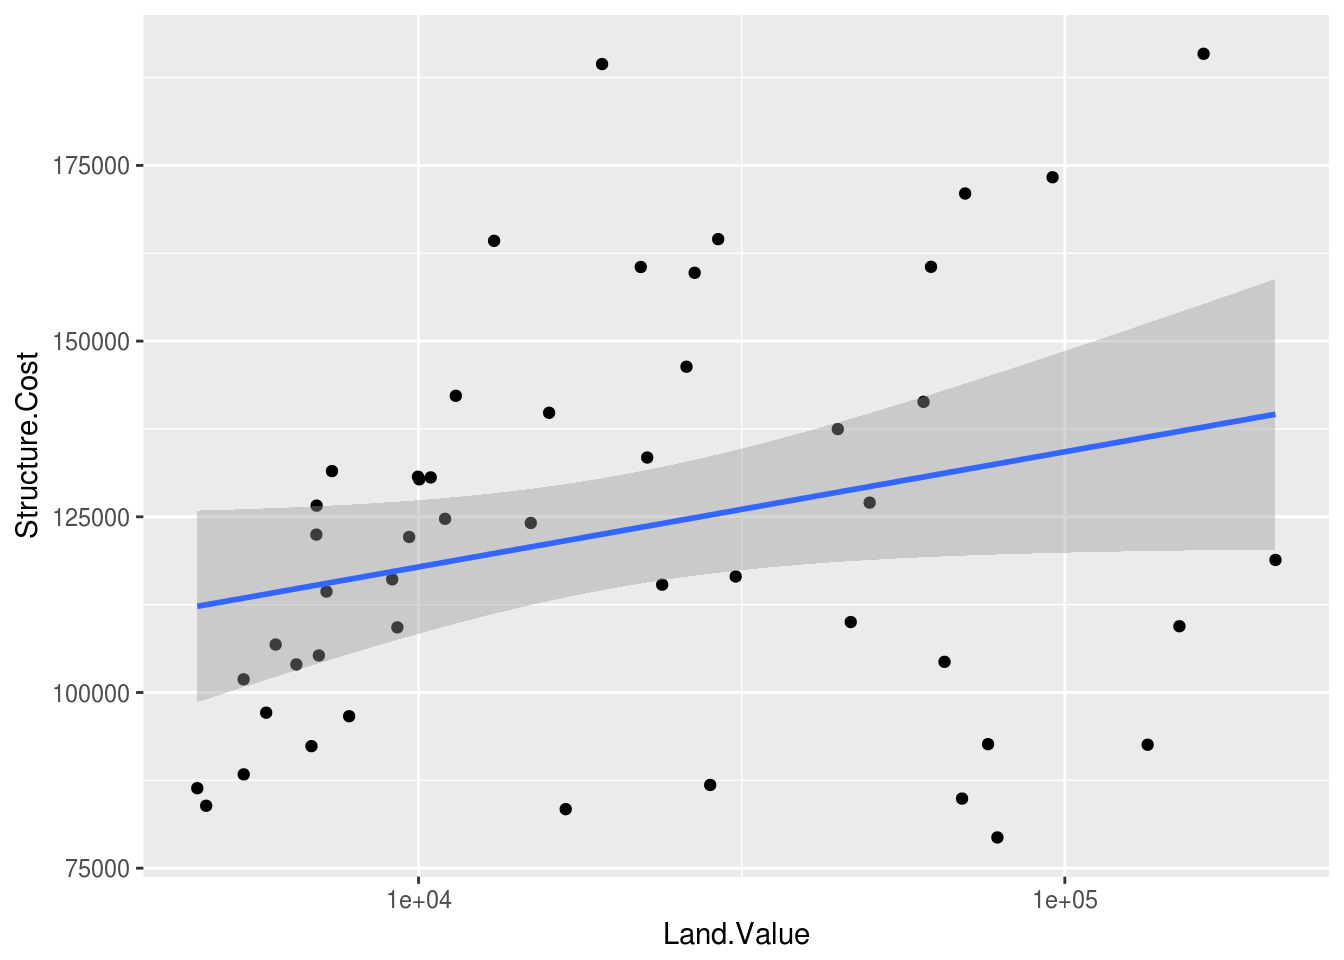
\includegraphics{ggplot_tutorial_files/figure-latex/unnamed-chunk-36-1.pdf}

We can also specify the formula for the model

\begin{Shaded}
\begin{Highlighting}[]
\KeywordTok{ggplot}\NormalTok{(housing2001q1, }\KeywordTok{aes}\NormalTok{(}\DataTypeTok{x =} \NormalTok{Land.Value, }\DataTypeTok{y =} \NormalTok{Structure.Cost)) +}\StringTok{ }
\StringTok{  }\KeywordTok{geom_point}\NormalTok{() +}
\StringTok{  }\KeywordTok{scale_x_log10}\NormalTok{() +}
\StringTok{  }\KeywordTok{stat_smooth}\NormalTok{(}\DataTypeTok{method =} \StringTok{"lm"}\NormalTok{, }\DataTypeTok{formula =} \NormalTok{y ~}\StringTok{ }\KeywordTok{log}\NormalTok{(x))}
\end{Highlighting}
\end{Shaded}

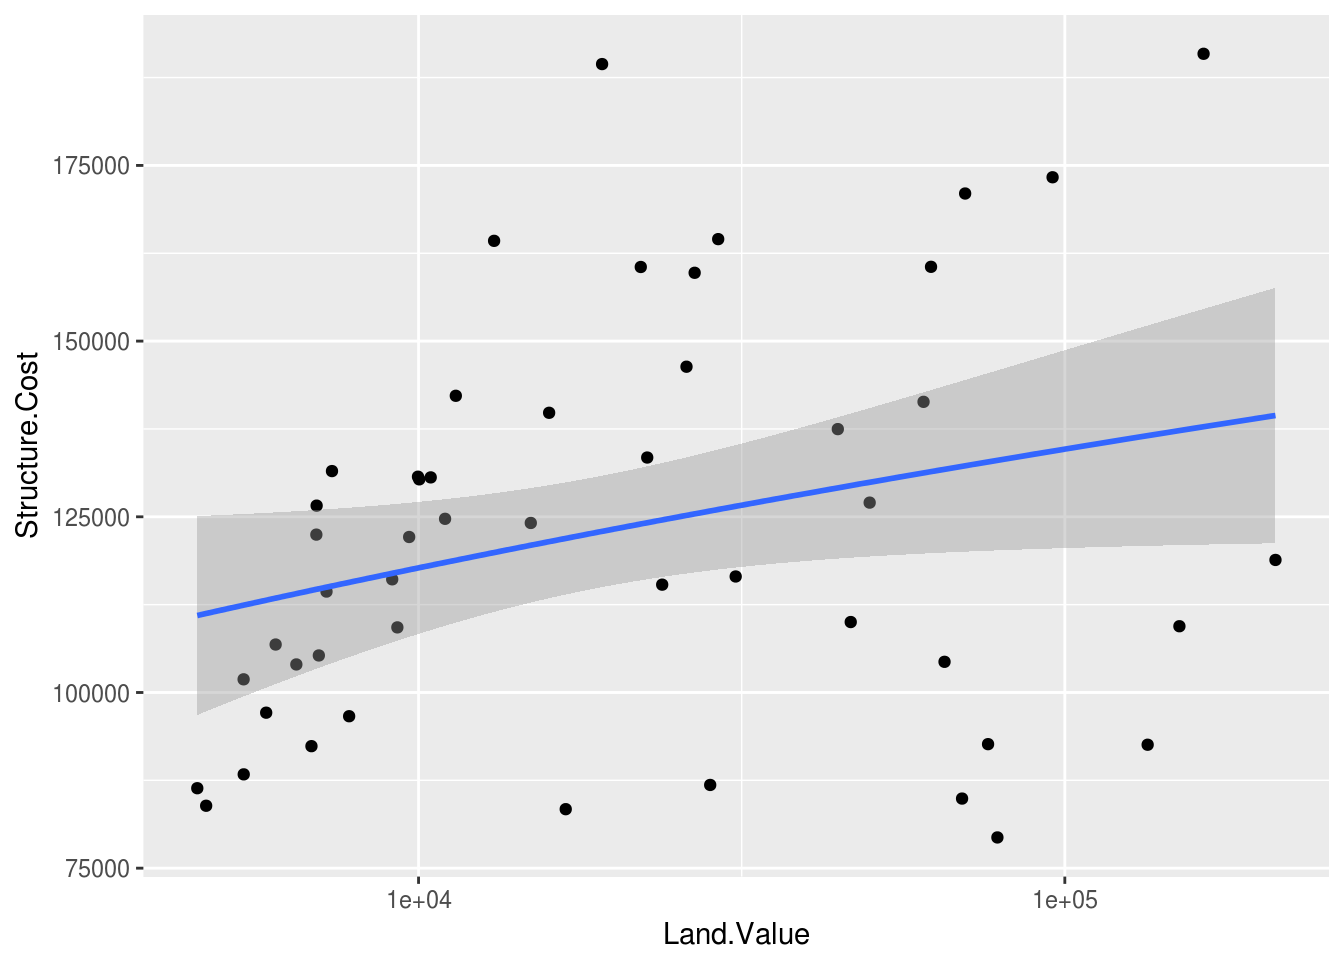
\includegraphics{ggplot_tutorial_files/figure-latex/unnamed-chunk-37-1.pdf}

We can turn the turn off the confidence interval

\begin{Shaded}
\begin{Highlighting}[]
\KeywordTok{ggplot}\NormalTok{(housing2001q1, }\KeywordTok{aes}\NormalTok{(}\DataTypeTok{x =} \NormalTok{Land.Value, }\DataTypeTok{y =} \NormalTok{Structure.Cost)) +}\StringTok{ }
\StringTok{  }\KeywordTok{geom_point}\NormalTok{() +}
\StringTok{  }\KeywordTok{scale_x_log10}\NormalTok{() +}
\StringTok{  }\KeywordTok{stat_smooth}\NormalTok{(}\DataTypeTok{method =} \StringTok{"lm"}\NormalTok{, }\DataTypeTok{formula =} \NormalTok{y ~}\StringTok{ }\KeywordTok{log}\NormalTok{(x), }\DataTypeTok{se =} \OtherTok{FALSE}\NormalTok{)}
\end{Highlighting}
\end{Shaded}

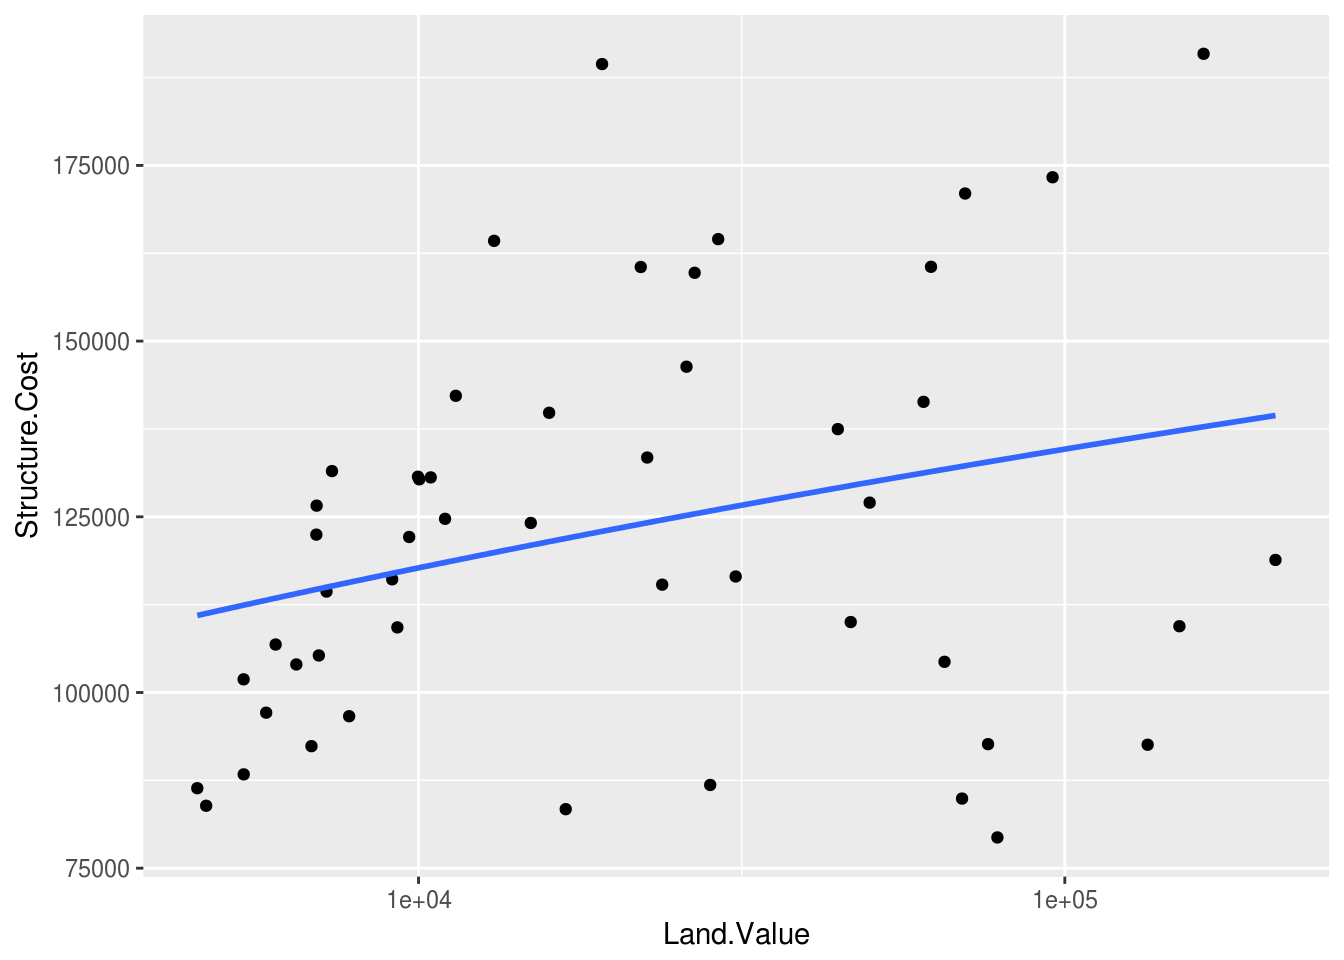
\includegraphics{ggplot_tutorial_files/figure-latex/unnamed-chunk-38-1.pdf}

Formula is specific to the type of model used. Here we're using a
General Additive Model (GAM).

\begin{Shaded}
\begin{Highlighting}[]
\KeywordTok{ggplot}\NormalTok{(housing2001q1, }\KeywordTok{aes}\NormalTok{(}\DataTypeTok{x =} \NormalTok{Land.Value, }\DataTypeTok{y =} \NormalTok{Structure.Cost)) +}\StringTok{ }
\StringTok{  }\KeywordTok{geom_point}\NormalTok{() +}
\StringTok{  }\KeywordTok{scale_x_log10}\NormalTok{() +}
\StringTok{  }\KeywordTok{stat_smooth}\NormalTok{(}\DataTypeTok{method =} \StringTok{"gam"}\NormalTok{, }\DataTypeTok{formula =} \NormalTok{y ~}\StringTok{ }\KeywordTok{s}\NormalTok{(x,}\DataTypeTok{k=}\DecValTok{10}\NormalTok{))}
\end{Highlighting}
\end{Shaded}

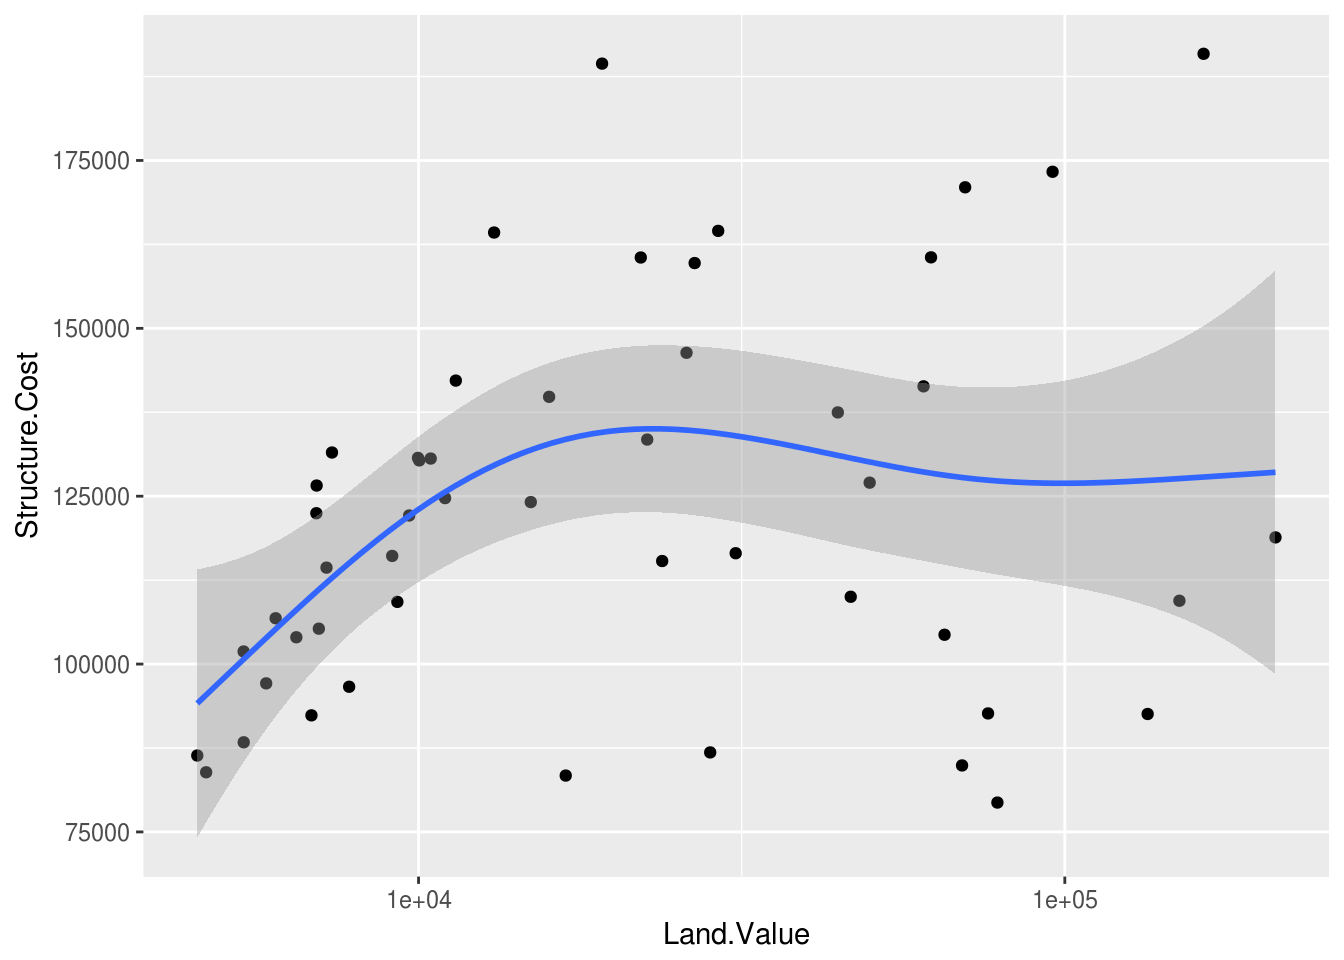
\includegraphics{ggplot_tutorial_files/figure-latex/unnamed-chunk-39-1.pdf}

\section{Theme and Title}\label{theme-and-title}

First, let's try some of the themes from the \texttt{ggthemes} package

\begin{Shaded}
\begin{Highlighting}[]
\KeywordTok{ggplot}\NormalTok{(northeast, }\KeywordTok{aes}\NormalTok{(}\DataTypeTok{x =} \NormalTok{Date, }\DataTypeTok{y =} \NormalTok{Home.Value, }\DataTypeTok{color =} \NormalTok{State)) +}
\StringTok{  }\KeywordTok{geom_line}\NormalTok{() +}
\StringTok{  }\KeywordTok{theme_stata}\NormalTok{()}
\end{Highlighting}
\end{Shaded}

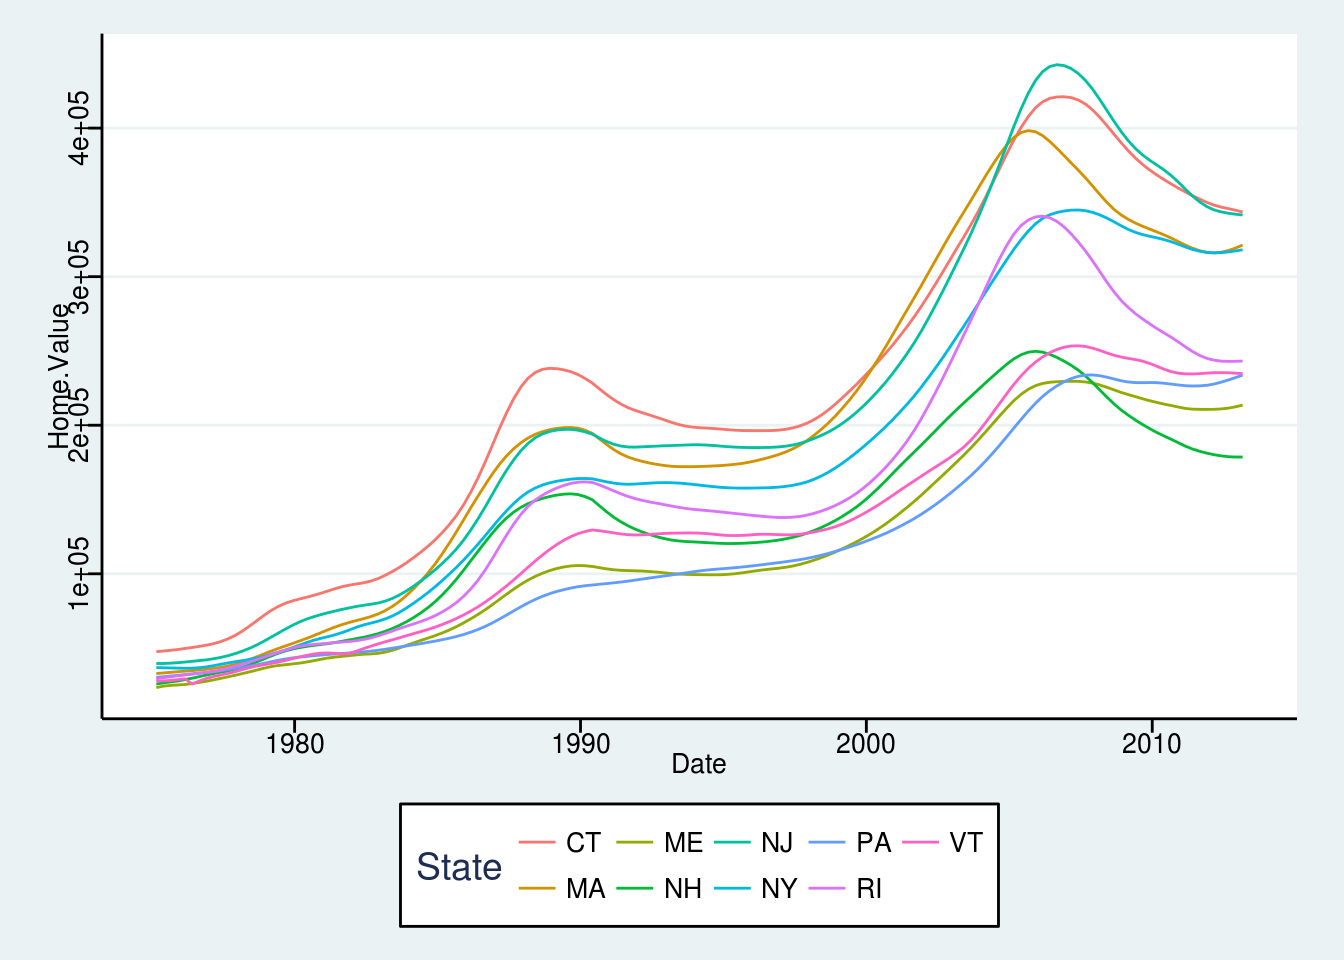
\includegraphics{ggplot_tutorial_files/figure-latex/unnamed-chunk-40-1.pdf}

\begin{Shaded}
\begin{Highlighting}[]
\KeywordTok{ggplot}\NormalTok{(northeast, }\KeywordTok{aes}\NormalTok{(}\DataTypeTok{x =} \NormalTok{Date, }\DataTypeTok{y =} \NormalTok{Home.Value, }\DataTypeTok{color =} \NormalTok{State)) +}
\StringTok{  }\KeywordTok{geom_line}\NormalTok{() +}
\StringTok{  }\KeywordTok{theme_economist}\NormalTok{()}
\end{Highlighting}
\end{Shaded}

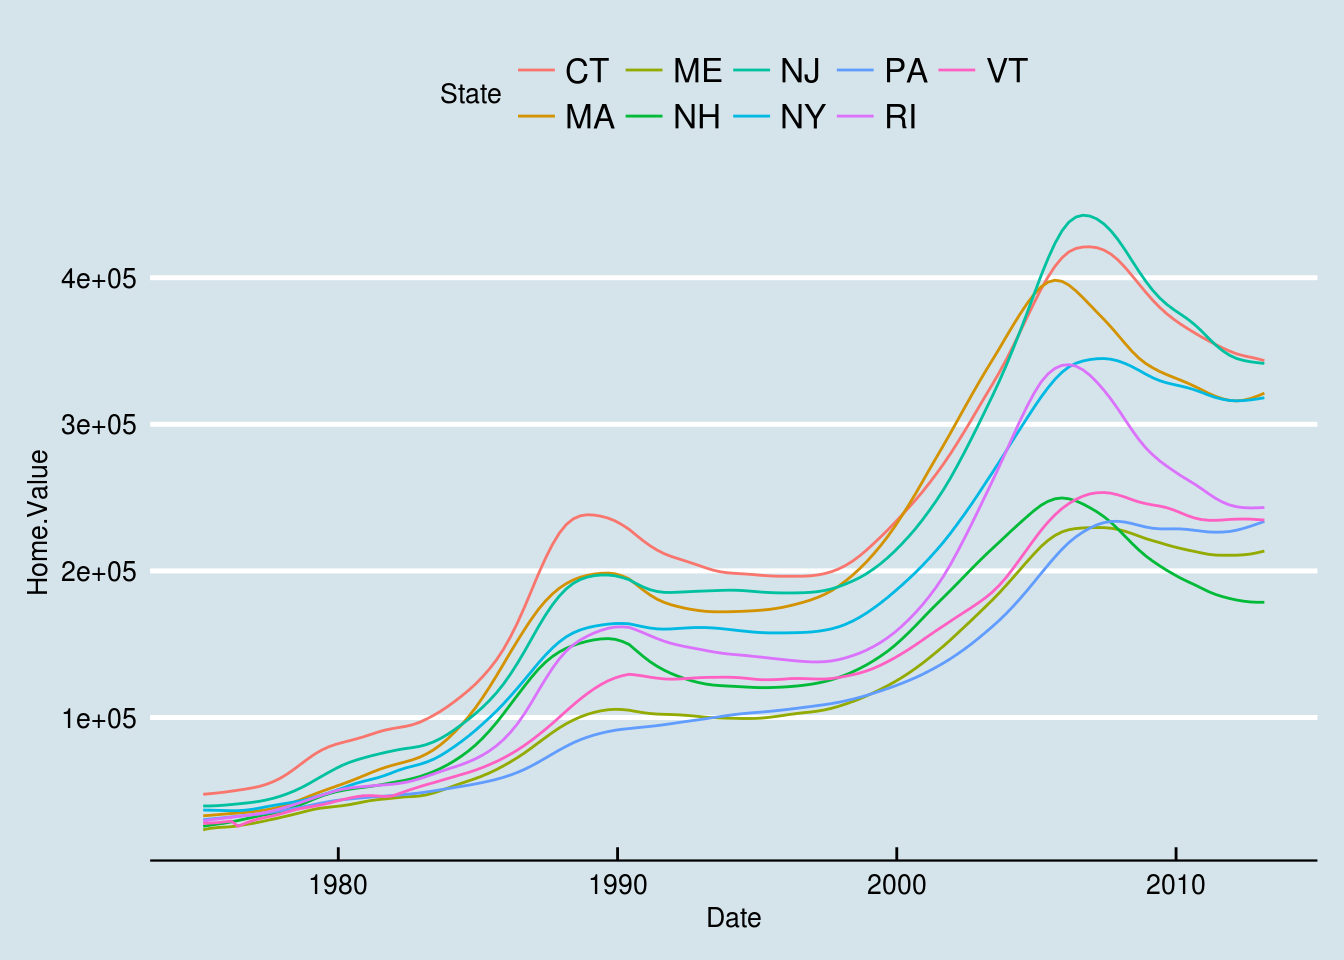
\includegraphics{ggplot_tutorial_files/figure-latex/unnamed-chunk-41-1.pdf}

\begin{Shaded}
\begin{Highlighting}[]
\KeywordTok{ggplot}\NormalTok{(northeast, }\KeywordTok{aes}\NormalTok{(}\DataTypeTok{x =} \NormalTok{Date, }\DataTypeTok{y =} \NormalTok{Home.Value, }\DataTypeTok{color =} \NormalTok{State)) +}
\StringTok{  }\KeywordTok{geom_line}\NormalTok{() +}
\StringTok{  }\KeywordTok{theme_wsj}\NormalTok{()}
\end{Highlighting}
\end{Shaded}

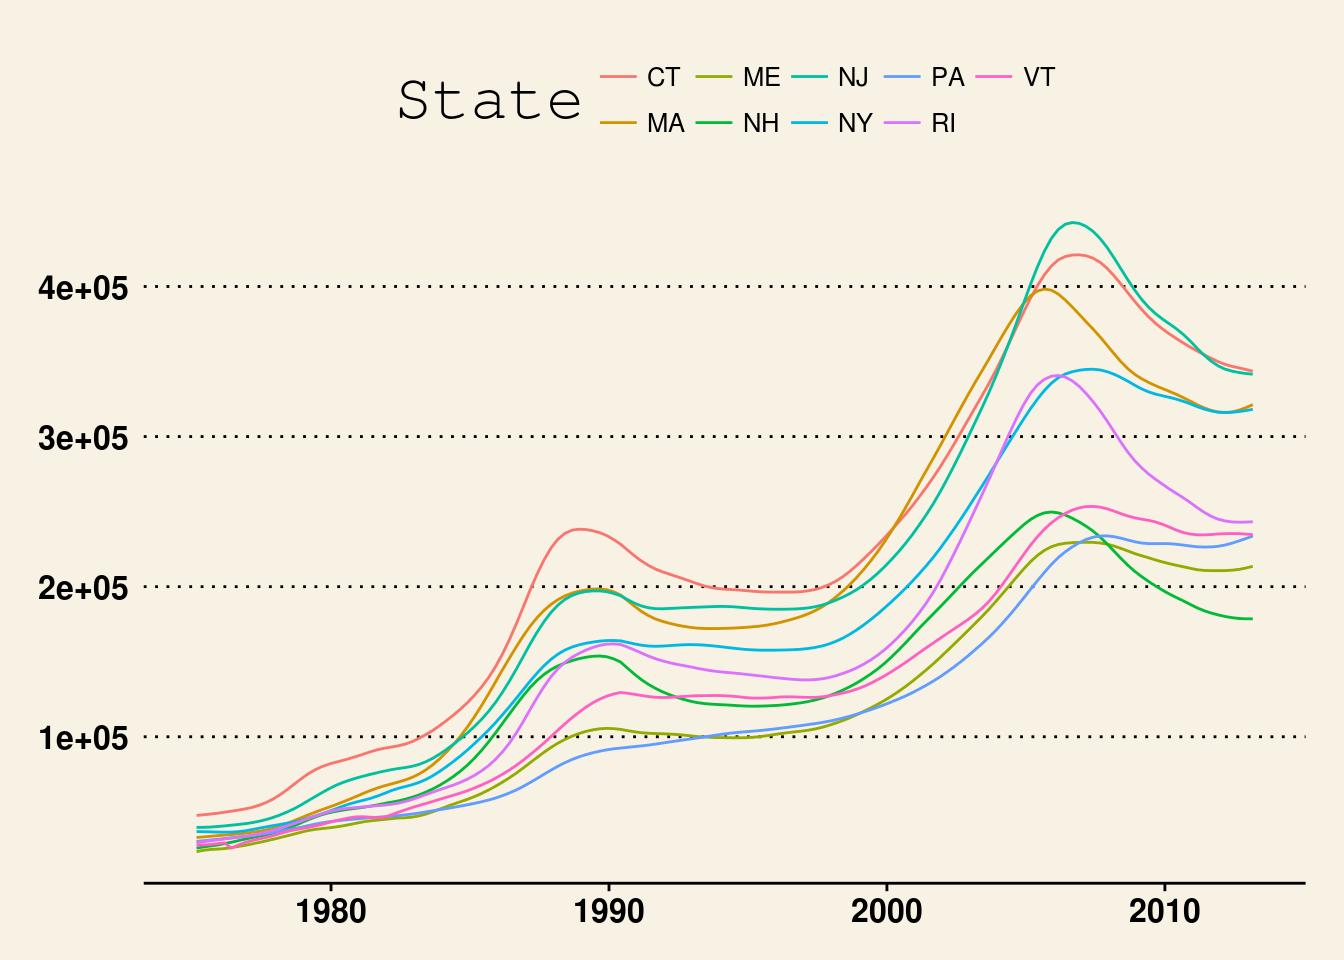
\includegraphics{ggplot_tutorial_files/figure-latex/unnamed-chunk-42-1.pdf}

\begin{Shaded}
\begin{Highlighting}[]
\KeywordTok{ggplot}\NormalTok{(northeast, }\KeywordTok{aes}\NormalTok{(}\DataTypeTok{x =} \NormalTok{Date, }\DataTypeTok{y =} \NormalTok{Home.Value, }\DataTypeTok{color =} \NormalTok{State)) +}
\StringTok{  }\KeywordTok{geom_line}\NormalTok{() +}
\StringTok{  }\KeywordTok{theme_solarized}\NormalTok{()}
\end{Highlighting}
\end{Shaded}

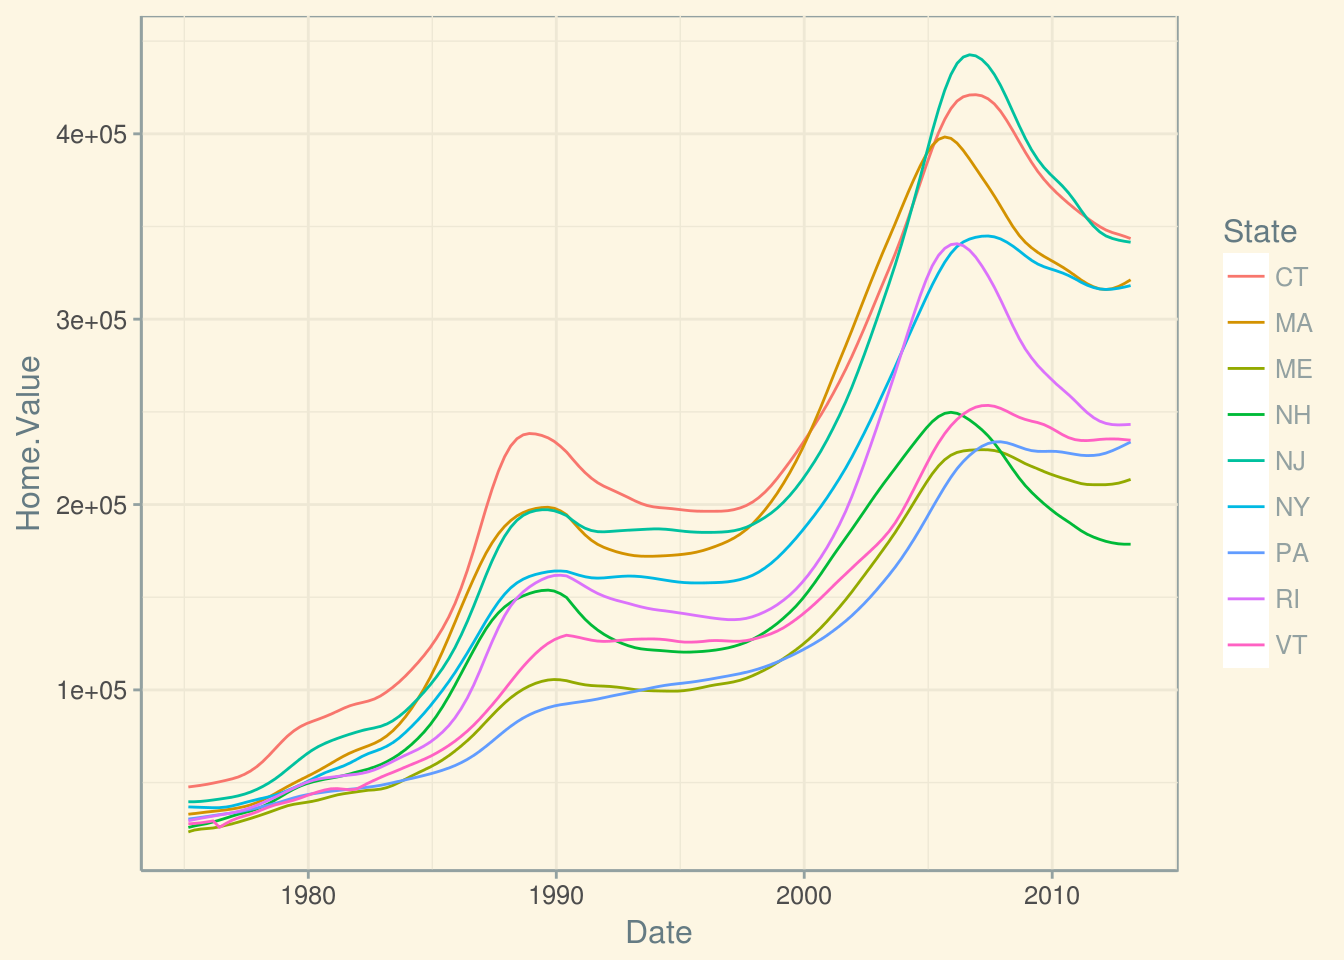
\includegraphics{ggplot_tutorial_files/figure-latex/unnamed-chunk-43-1.pdf}

\begin{Shaded}
\begin{Highlighting}[]
\KeywordTok{ggplot}\NormalTok{(northeast, }\KeywordTok{aes}\NormalTok{(}\DataTypeTok{x =} \NormalTok{Date, }\DataTypeTok{y =} \NormalTok{Home.Value, }\DataTypeTok{color =} \NormalTok{State)) +}
\StringTok{  }\KeywordTok{geom_line}\NormalTok{() +}
\StringTok{  }\KeywordTok{theme_fivethirtyeight}\NormalTok{()}
\end{Highlighting}
\end{Shaded}

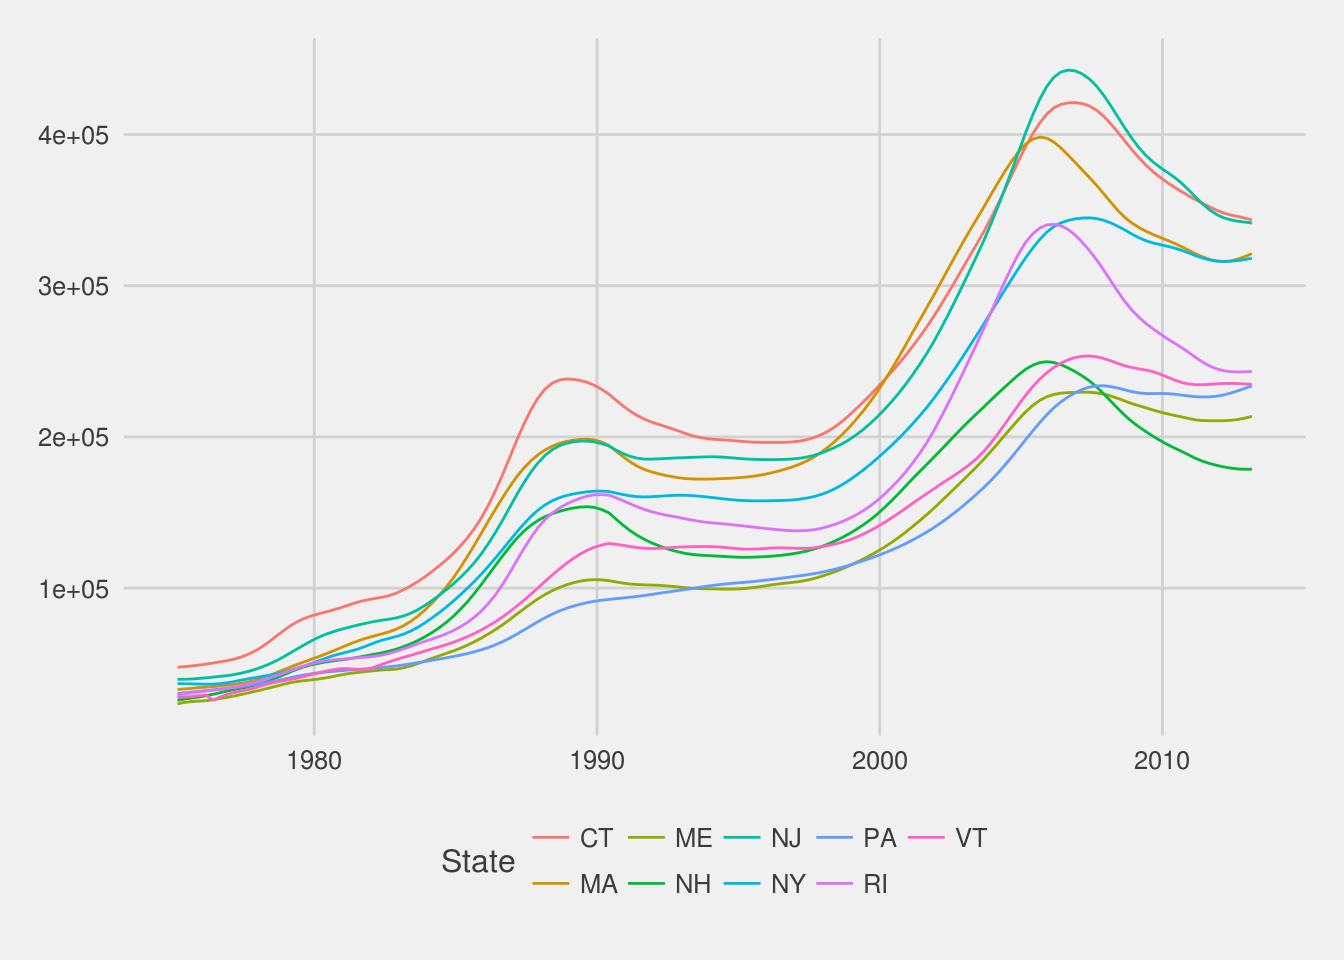
\includegraphics{ggplot_tutorial_files/figure-latex/unnamed-chunk-44-1.pdf}

We can also have complete control over the theme by customizing each
element ourselves. Let's start with \texttt{theme\_minimal()}

\begin{Shaded}
\begin{Highlighting}[]
\KeywordTok{ggplot}\NormalTok{(northeast, }\KeywordTok{aes}\NormalTok{(}\DataTypeTok{x =} \NormalTok{Date, }\DataTypeTok{y =} \NormalTok{Home.Value, }\DataTypeTok{color =} \NormalTok{State)) +}
\StringTok{  }\KeywordTok{geom_line}\NormalTok{() +}
\StringTok{  }\KeywordTok{theme_minimal}\NormalTok{()}
\end{Highlighting}
\end{Shaded}

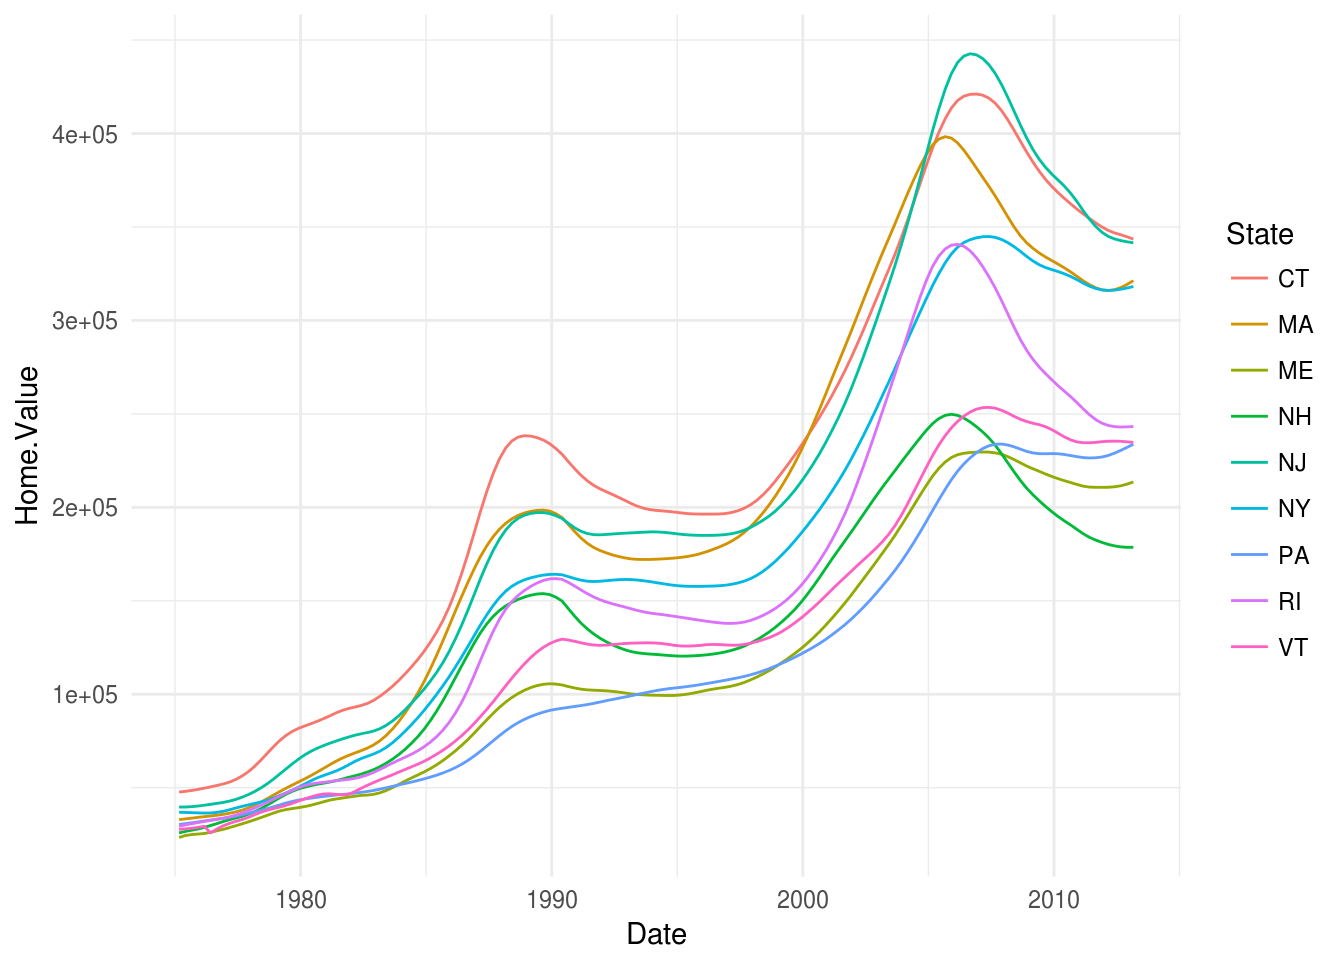
\includegraphics{ggplot_tutorial_files/figure-latex/unnamed-chunk-45-1.pdf}

Now remove the minor grid lines

\begin{Shaded}
\begin{Highlighting}[]
\KeywordTok{ggplot}\NormalTok{(northeast, }\KeywordTok{aes}\NormalTok{(}\DataTypeTok{x =} \NormalTok{Date, }\DataTypeTok{y =} \NormalTok{Home.Value, }\DataTypeTok{color =} \NormalTok{State)) +}
\StringTok{  }\KeywordTok{geom_line}\NormalTok{() +}
\StringTok{  }\KeywordTok{theme_minimal}\NormalTok{() +}
\StringTok{  }\KeywordTok{theme}\NormalTok{(}
    \DataTypeTok{panel.grid.minor =} \KeywordTok{element_blank}\NormalTok{()}
  \NormalTok{)}
\end{Highlighting}
\end{Shaded}

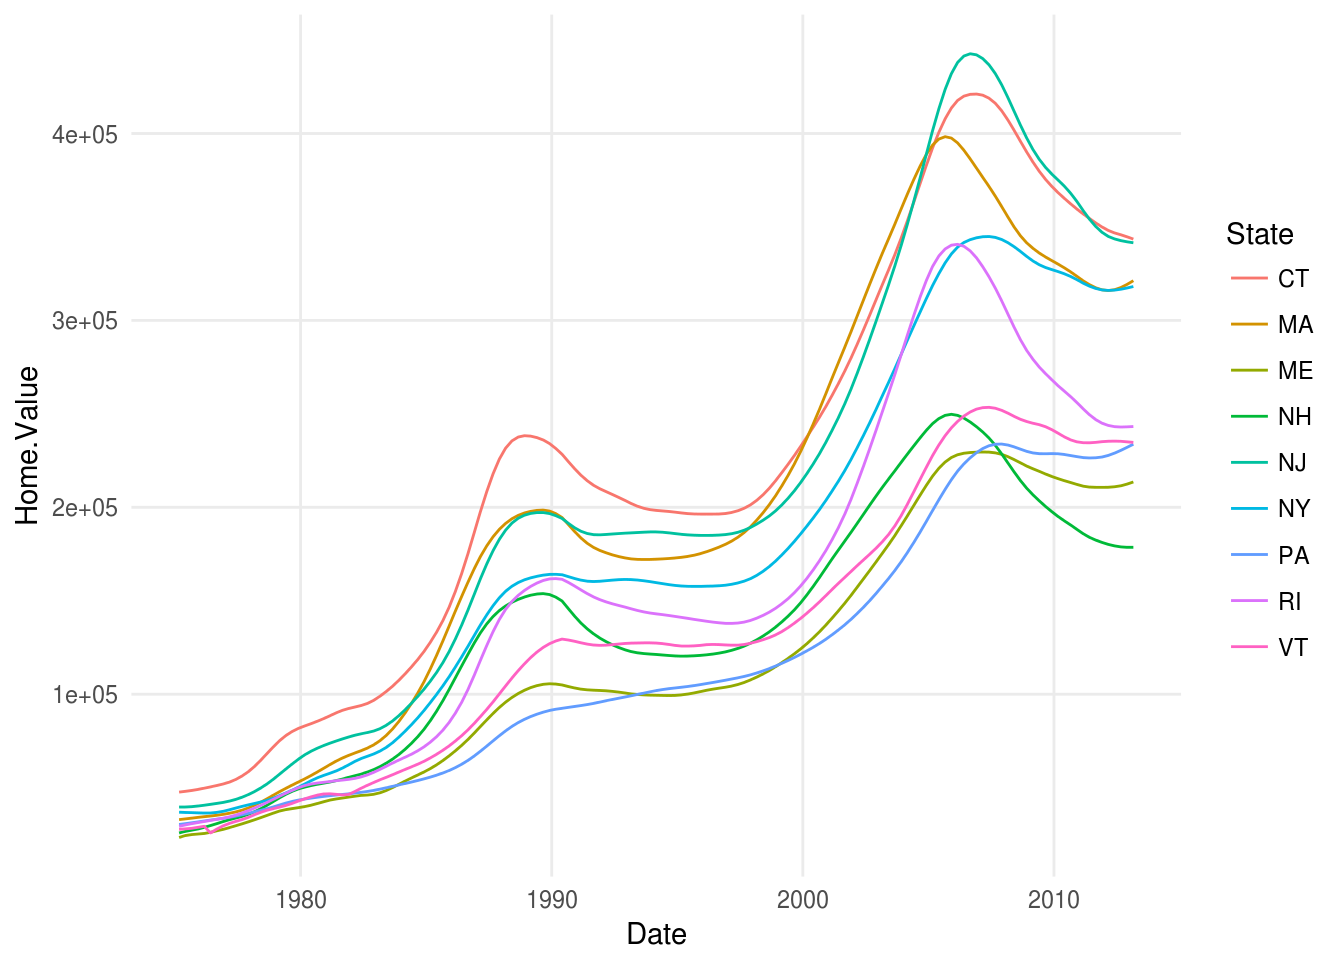
\includegraphics{ggplot_tutorial_files/figure-latex/unnamed-chunk-46-1.pdf}

Next, we change the y-axis label

\begin{Shaded}
\begin{Highlighting}[]
\KeywordTok{ggplot}\NormalTok{(northeast, }\KeywordTok{aes}\NormalTok{(}\DataTypeTok{x =} \NormalTok{Date, }\DataTypeTok{y =} \NormalTok{Home.Value, }\DataTypeTok{color =} \NormalTok{State)) +}
\StringTok{  }\KeywordTok{geom_line}\NormalTok{() +}
\StringTok{  }\KeywordTok{theme_minimal}\NormalTok{() +}
\StringTok{  }\KeywordTok{theme}\NormalTok{(}
    \DataTypeTok{panel.grid.minor =} \KeywordTok{element_blank}\NormalTok{()}
  \NormalTok{) +}
\StringTok{  }\KeywordTok{ylab}\NormalTok{(}\StringTok{"Home Value (US$)"}\NormalTok{)}
\end{Highlighting}
\end{Shaded}

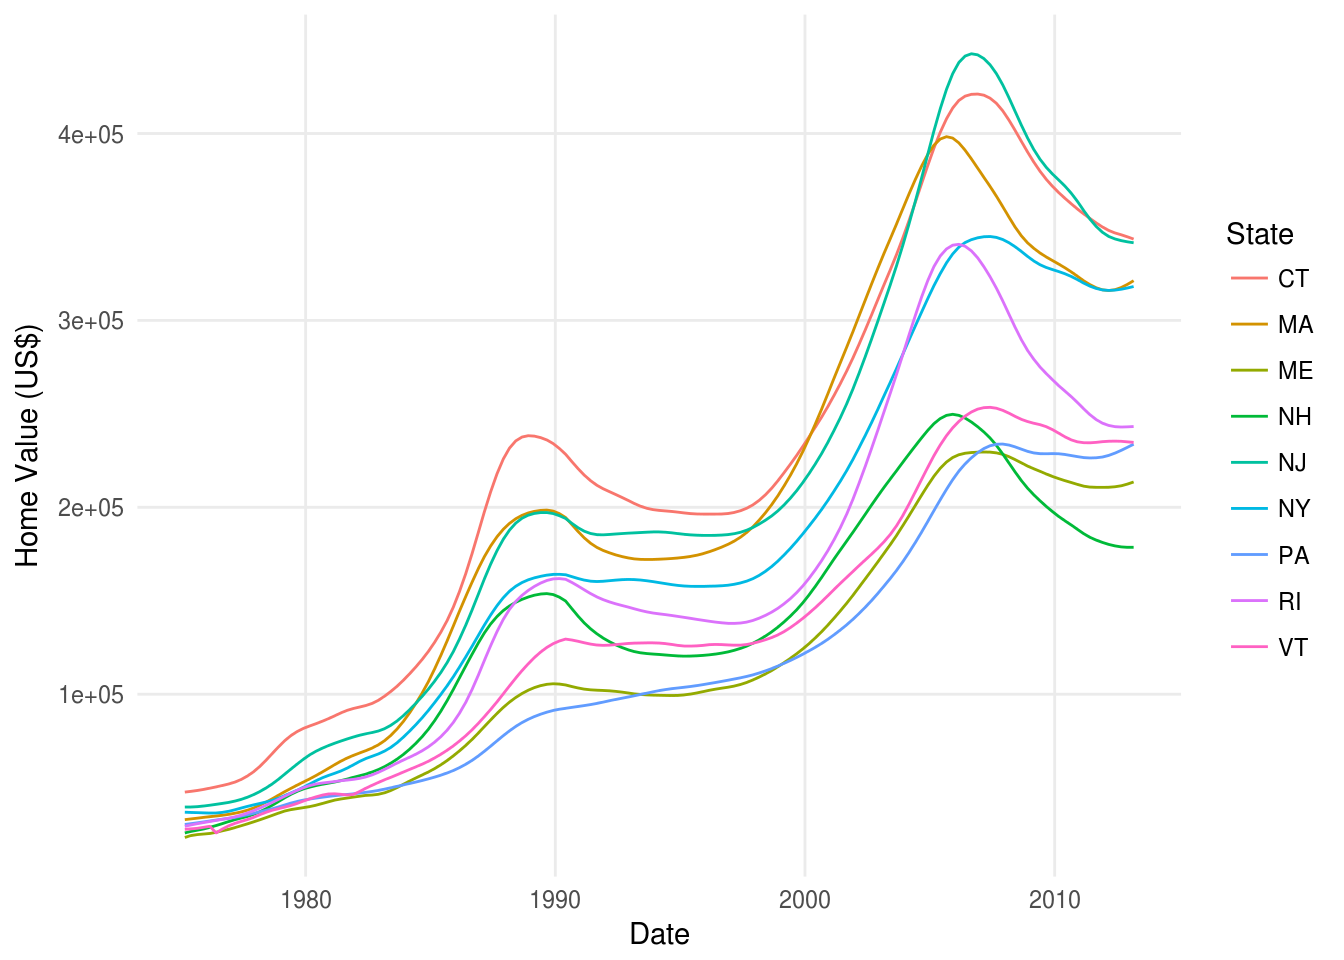
\includegraphics{ggplot_tutorial_files/figure-latex/unnamed-chunk-47-1.pdf}

Then remove the x-axis title since the year is self explanatory

\begin{Shaded}
\begin{Highlighting}[]
\KeywordTok{ggplot}\NormalTok{(northeast, }\KeywordTok{aes}\NormalTok{(}\DataTypeTok{x =} \NormalTok{Date, }\DataTypeTok{y =} \NormalTok{Home.Value, }\DataTypeTok{color =} \NormalTok{State)) +}
\StringTok{  }\KeywordTok{geom_line}\NormalTok{() +}
\StringTok{  }\KeywordTok{theme_minimal}\NormalTok{() +}
\StringTok{  }\KeywordTok{theme}\NormalTok{(}
    \DataTypeTok{axis.title.x =} \KeywordTok{element_blank}\NormalTok{(),}
    \DataTypeTok{panel.grid.minor =} \KeywordTok{element_blank}\NormalTok{()}
  \NormalTok{) +}
\StringTok{  }\KeywordTok{ylab}\NormalTok{(}\StringTok{"Home Value (US$)"}\NormalTok{)}
\end{Highlighting}
\end{Shaded}

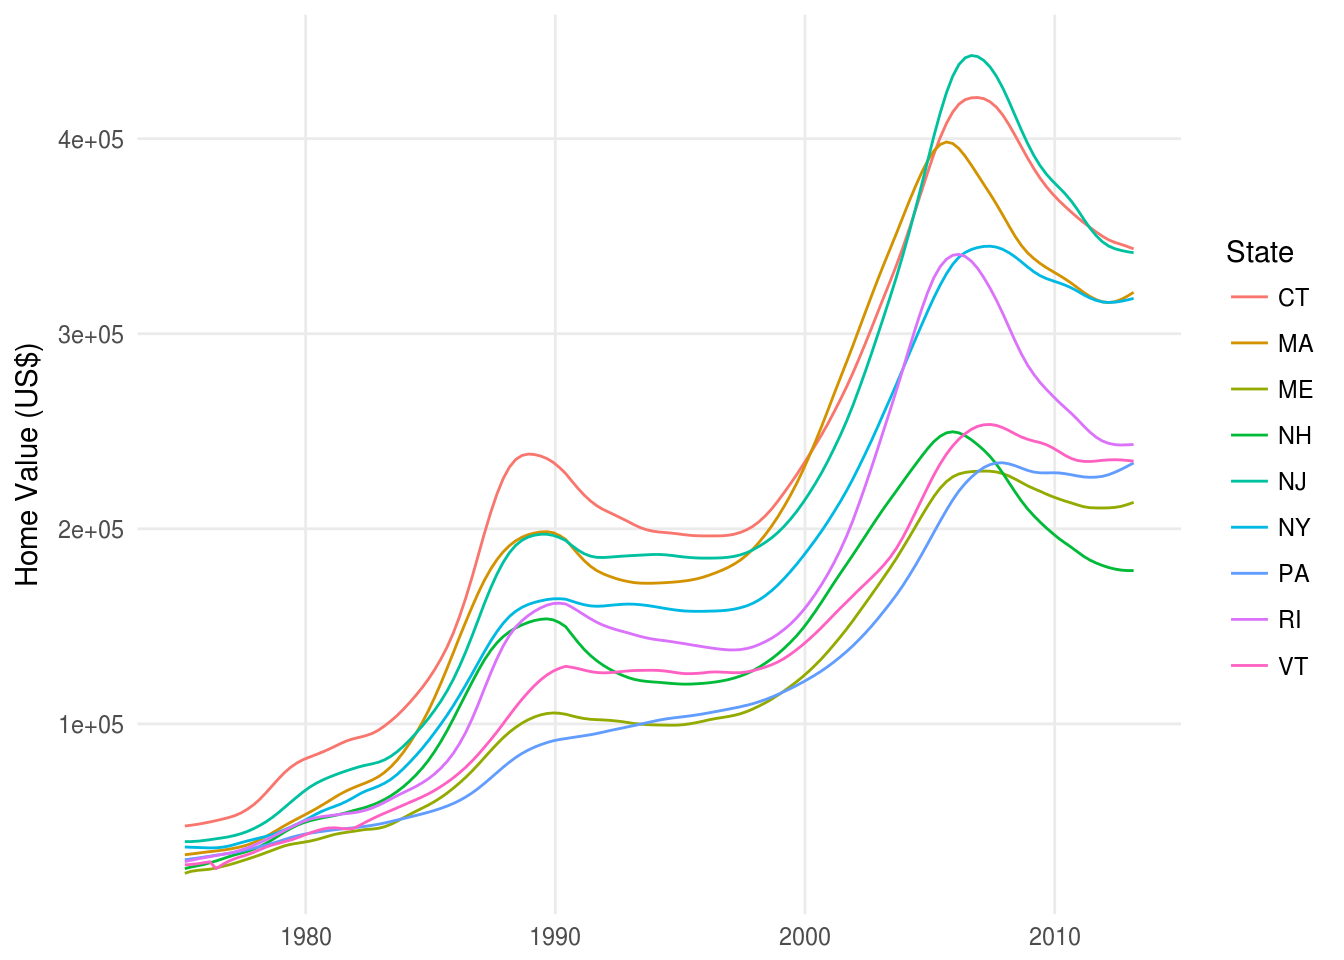
\includegraphics{ggplot_tutorial_files/figure-latex/unnamed-chunk-48-1.pdf}

Finally, we can add a title to our plot

\begin{Shaded}
\begin{Highlighting}[]
\KeywordTok{ggplot}\NormalTok{(northeast, }\KeywordTok{aes}\NormalTok{(}\DataTypeTok{x =} \NormalTok{Date, }\DataTypeTok{y =} \NormalTok{Home.Value, }\DataTypeTok{color =} \NormalTok{State)) +}
\StringTok{  }\KeywordTok{geom_line}\NormalTok{() +}
\StringTok{  }\KeywordTok{theme_minimal}\NormalTok{() +}
\StringTok{  }\KeywordTok{theme}\NormalTok{(}
    \DataTypeTok{axis.title.x =} \KeywordTok{element_blank}\NormalTok{(),}
    \DataTypeTok{panel.grid.minor =} \KeywordTok{element_blank}\NormalTok{()}
  \NormalTok{) +}
\StringTok{  }\KeywordTok{ylab}\NormalTok{(}\StringTok{"Home Value (US$)"}\NormalTok{) +}
\StringTok{  }\KeywordTok{ggtitle}\NormalTok{(}\StringTok{"Housing Market in New York (1975 - 2013)"}\NormalTok{)}
\end{Highlighting}
\end{Shaded}

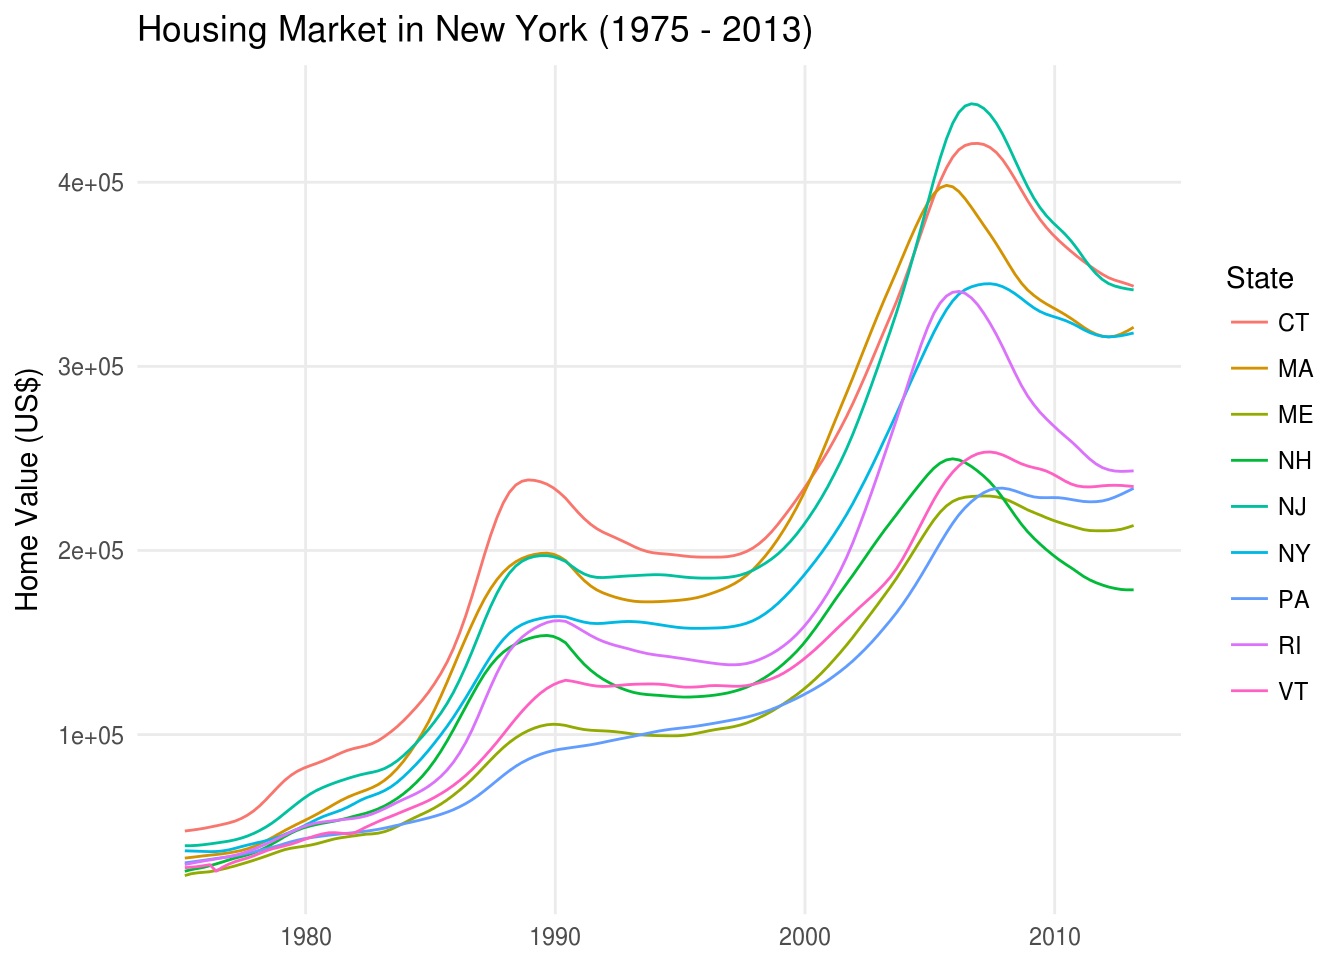
\includegraphics{ggplot_tutorial_files/figure-latex/unnamed-chunk-49-1.pdf}

\section{Facets}\label{facets}

Let's plot the northeast data again

\begin{Shaded}
\begin{Highlighting}[]
\KeywordTok{ggplot}\NormalTok{(northeast, }\KeywordTok{aes}\NormalTok{(}\DataTypeTok{x =} \NormalTok{Date, }\DataTypeTok{y =} \NormalTok{Home.Value, }\DataTypeTok{color =} \NormalTok{State)) +}
\StringTok{  }\KeywordTok{geom_line}\NormalTok{()}
\end{Highlighting}
\end{Shaded}

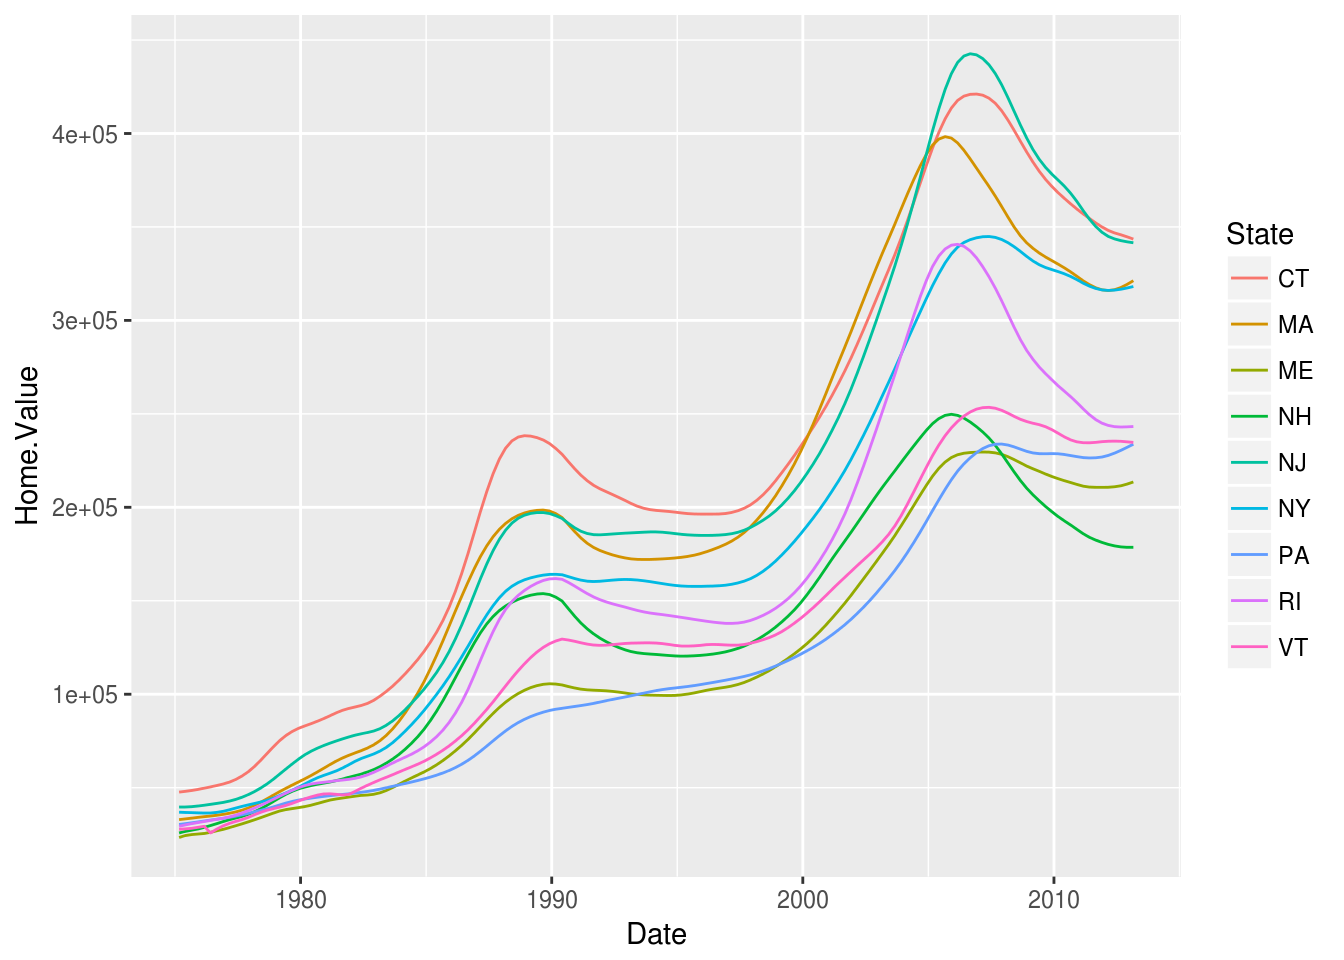
\includegraphics{ggplot_tutorial_files/figure-latex/unnamed-chunk-50-1.pdf}

But what if we were to plot the entire dataset?

\begin{Shaded}
\begin{Highlighting}[]
\KeywordTok{ggplot}\NormalTok{(housing, }\KeywordTok{aes}\NormalTok{(}\DataTypeTok{x =} \NormalTok{Date, }\DataTypeTok{y =} \NormalTok{Home.Value, }\DataTypeTok{color =} \NormalTok{State)) +}
\StringTok{  }\KeywordTok{geom_line}\NormalTok{()}
\end{Highlighting}
\end{Shaded}

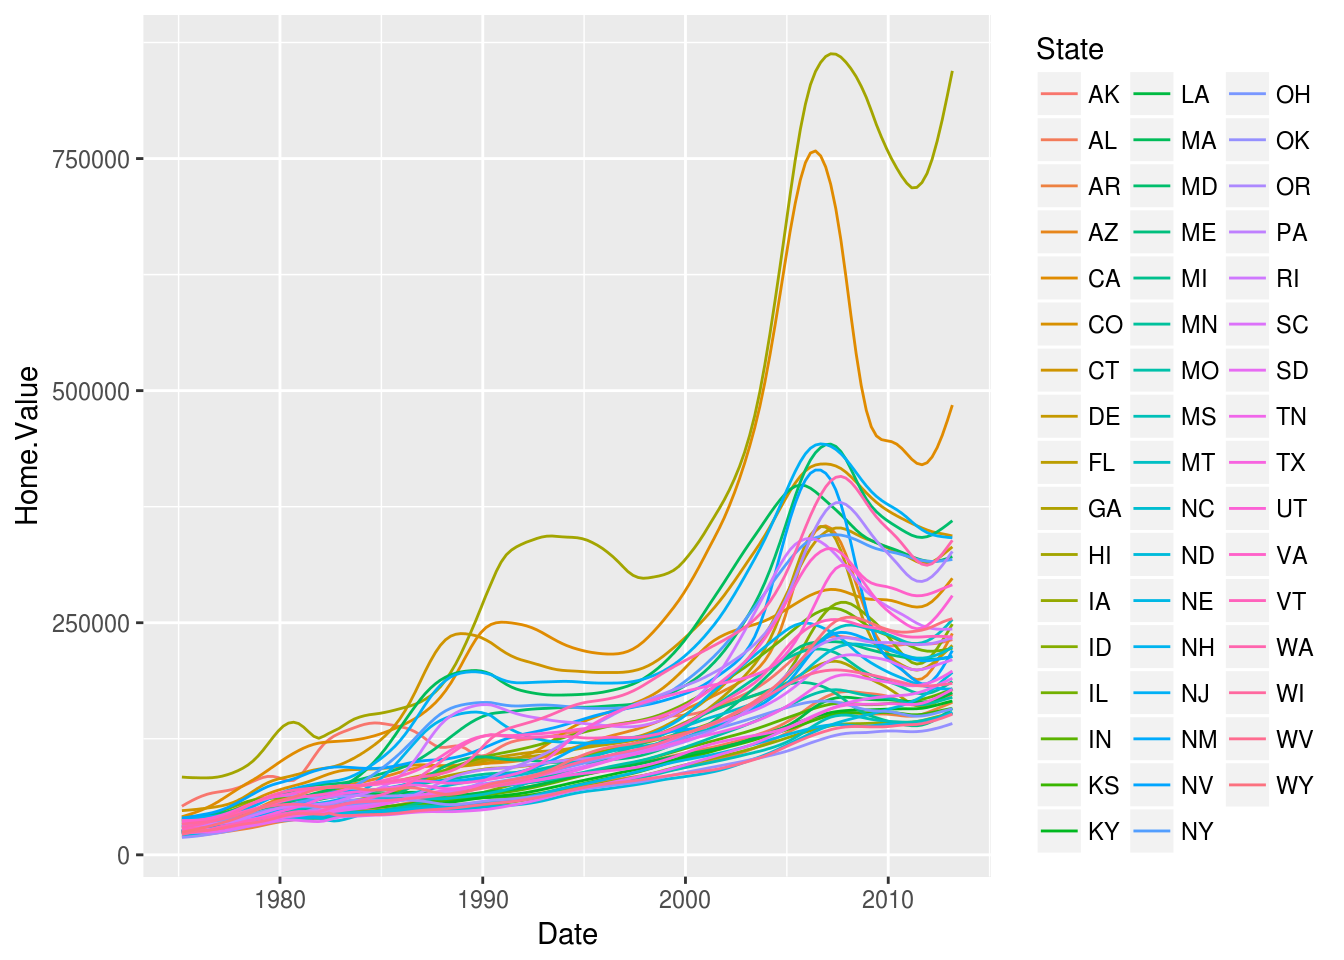
\includegraphics{ggplot_tutorial_files/figure-latex/unnamed-chunk-51-1.pdf}

The plot is not very informative anymore. We can use facets to split the
plot based on the \texttt{State}

\begin{Shaded}
\begin{Highlighting}[]
\KeywordTok{ggplot}\NormalTok{(northeast, }\KeywordTok{aes}\NormalTok{(}\DataTypeTok{x =} \NormalTok{Date, }\DataTypeTok{y =} \NormalTok{Home.Value)) +}
\StringTok{  }\KeywordTok{geom_line}\NormalTok{() +}
\StringTok{  }\KeywordTok{facet_wrap}\NormalTok{(~State, }\DataTypeTok{ncol =} \DecValTok{3}\NormalTok{)}
\end{Highlighting}
\end{Shaded}

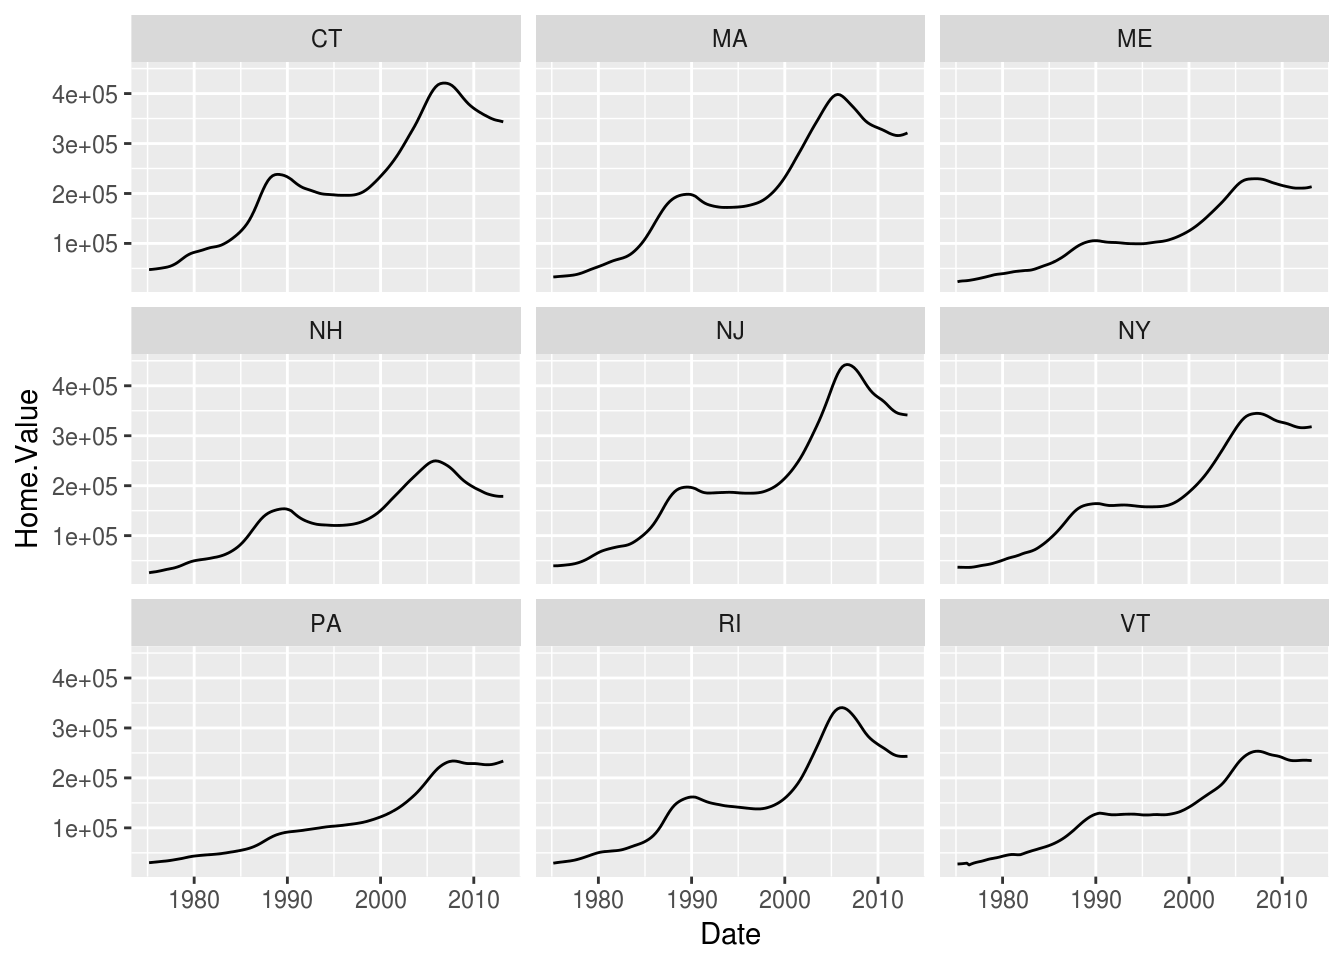
\includegraphics{ggplot_tutorial_files/figure-latex/unnamed-chunk-52-1.pdf}

\section{Challenge}\label{challenge}

\subsection{Recreating the Economist
Graph}\label{recreating-the-economist-graph}

\begin{figure}[htbp]
\centering
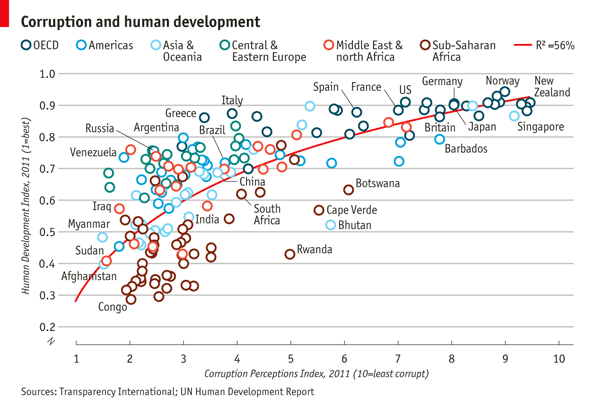
\includegraphics{./img/economist.png}
\caption{}
\end{figure}

\begin{Shaded}
\begin{Highlighting}[]
\NormalTok{econ <-}\StringTok{ }\KeywordTok{read.csv}\NormalTok{(}\StringTok{"https://raw.githubusercontent.com/altaf-ali/ggplot_tutorial/master/data/economist.csv"}\NormalTok{)}

\KeywordTok{head}\NormalTok{(econ)}
\end{Highlighting}
\end{Shaded}

\begin{verbatim}
##   X     Country HDI.Rank   HDI CPI            Region
## 1 1 Afghanistan      172 0.398 1.5      Asia Pacific
## 2 2     Albania       70 0.739 3.1 East EU Cemt Asia
## 3 3     Algeria       96 0.698 2.9              MENA
## 4 4      Angola      148 0.486 2.0               SSA
## 5 5   Argentina       45 0.797 3.0          Americas
## 6 6     Armenia       86 0.716 2.6 East EU Cemt Asia
\end{verbatim}

\begin{enumerate}
\def\labelenumi{\arabic{enumi}.}
\item
  Create a scatter plot of the economist data with \texttt{CPI} on the
  x-axis and \texttt{HDI} on the y-axis

  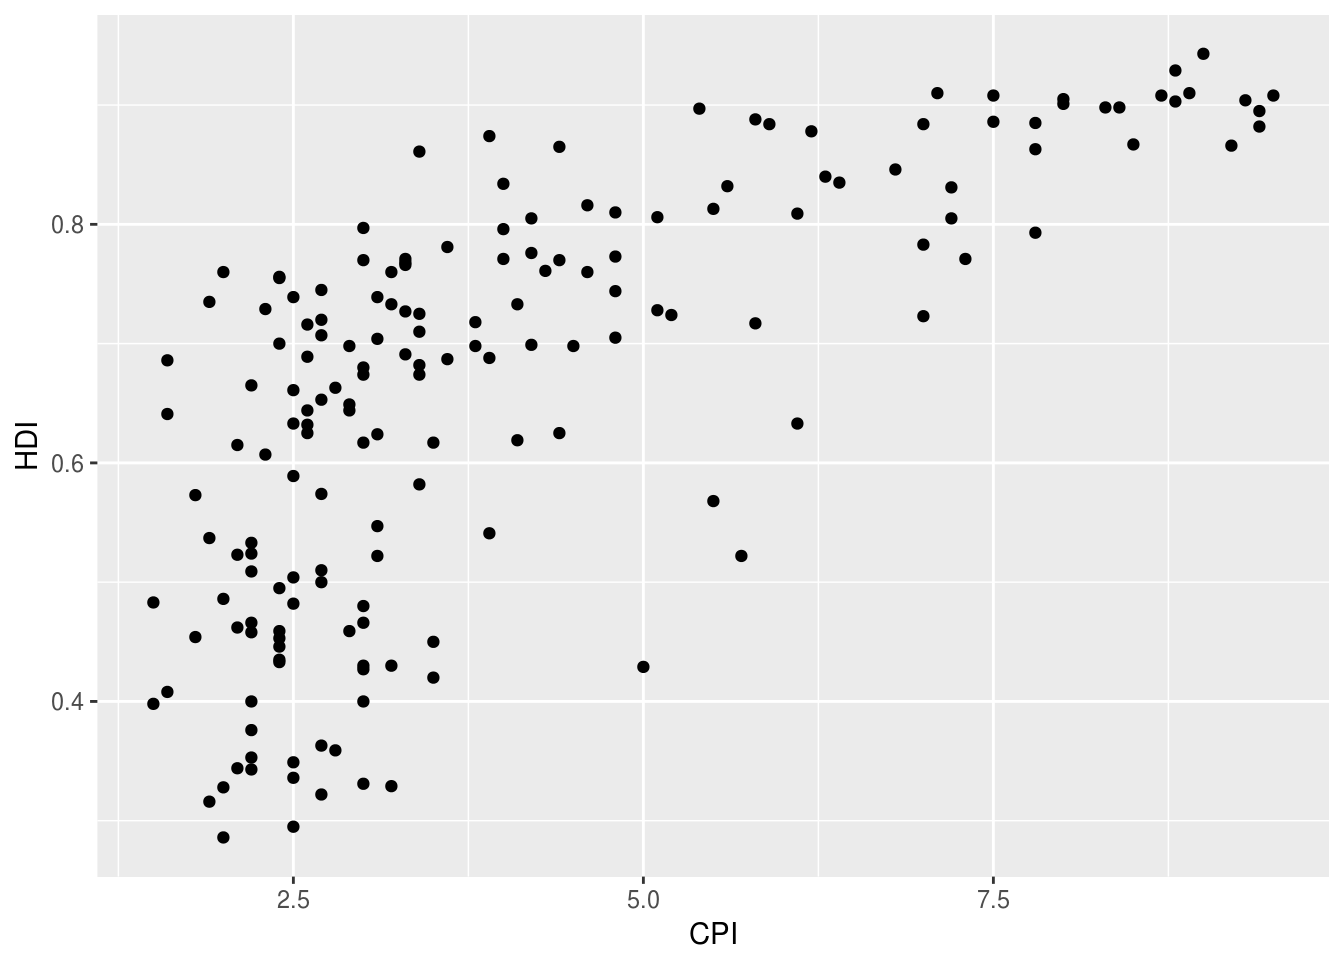
\includegraphics{ggplot_tutorial_files/figure-latex/unnamed-chunk-54-1.pdf}
\item
  Color the points based on \texttt{Region} using hollow points

  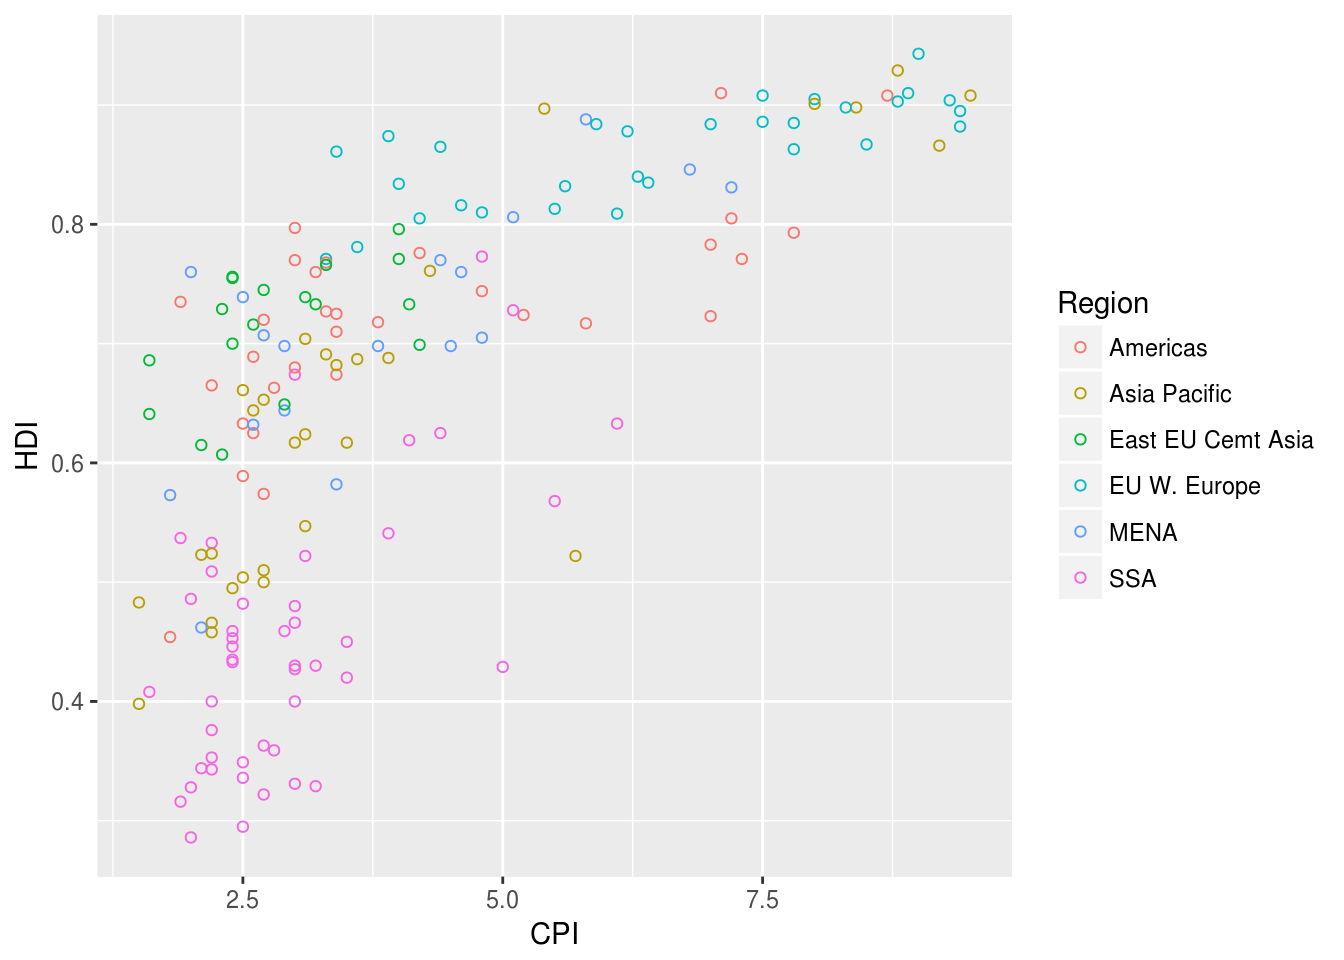
\includegraphics{ggplot_tutorial_files/figure-latex/unnamed-chunk-55-1.pdf}
\item
  Add a trend line

  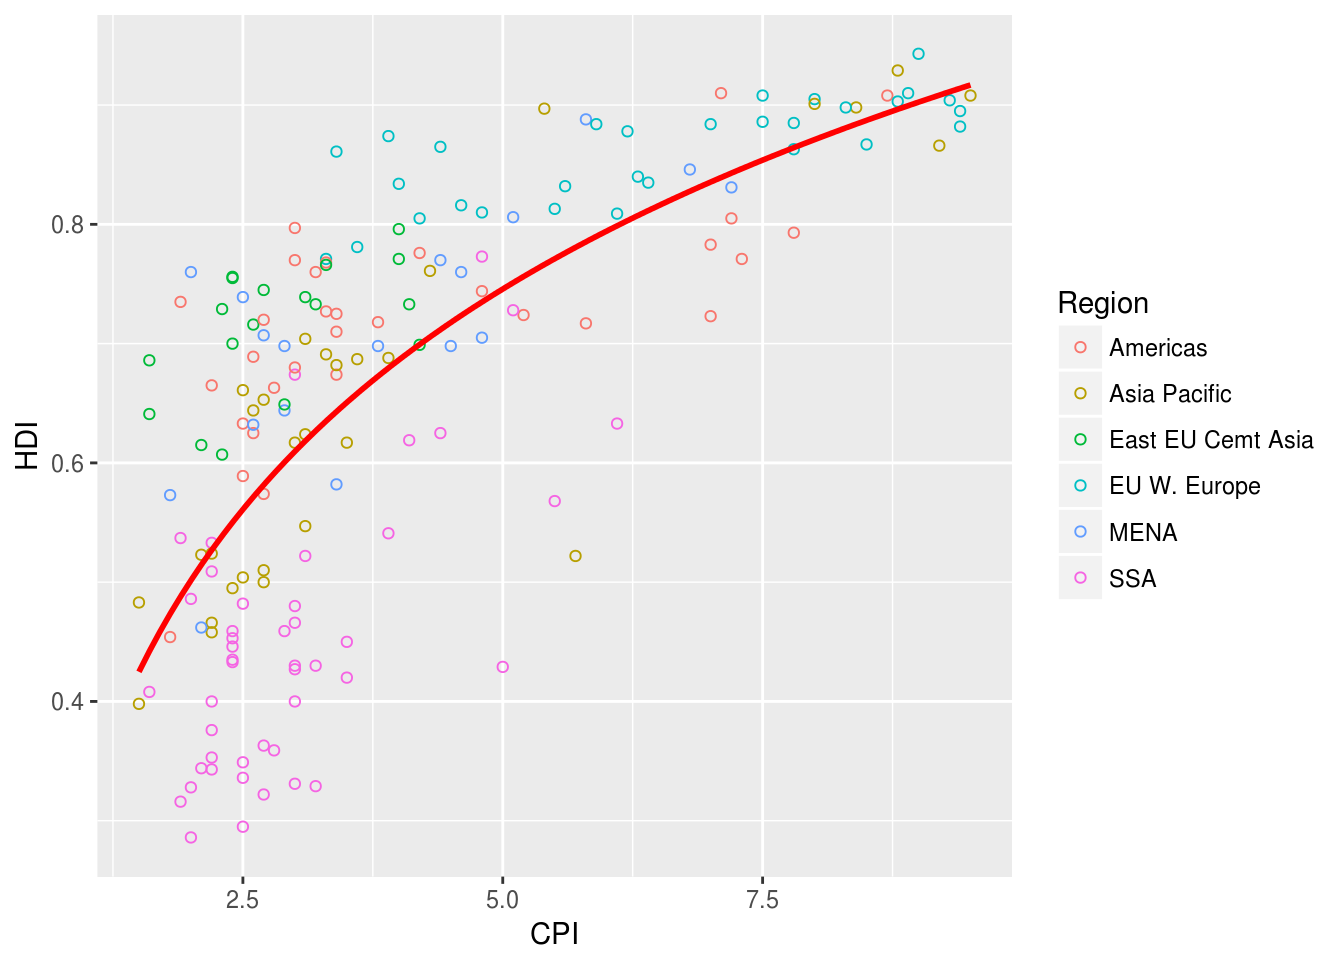
\includegraphics{ggplot_tutorial_files/figure-latex/unnamed-chunk-56-1.pdf}
\item
  The trend line is too thick compared to the circles so we need to
  adjust it appropriately

  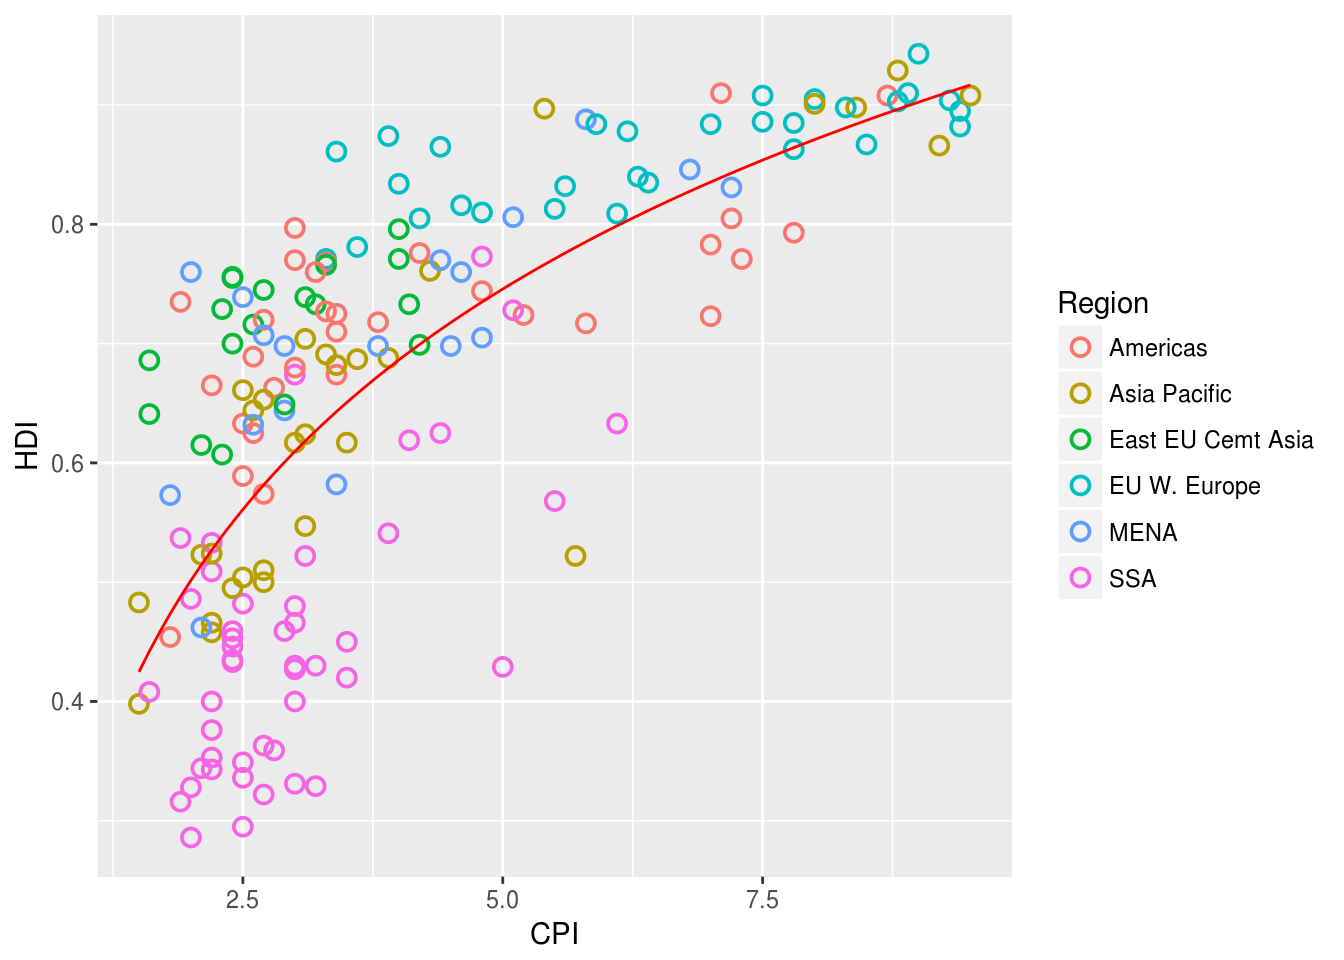
\includegraphics{ggplot_tutorial_files/figure-latex/unnamed-chunk-57-1.pdf}
\item
  Add text labels to the points

  HINT: Create a subset of countries to label since we don't want to
  label every point

\begin{Shaded}
\begin{Highlighting}[]
\NormalTok{target_countries <-}\StringTok{ }\KeywordTok{c}\NormalTok{(}
  \StringTok{"Russia"}\NormalTok{, }\StringTok{"Venezuela"}\NormalTok{, }\StringTok{"Iraq"}\NormalTok{, }\StringTok{"Myanmar"}\NormalTok{, }\StringTok{"Sudan"}\NormalTok{,}
  \StringTok{"Afghanistan"}\NormalTok{, }\StringTok{"Congo"}\NormalTok{, }\StringTok{"Greece"}\NormalTok{, }\StringTok{"Argentina"}\NormalTok{, }\StringTok{"Brazil"}\NormalTok{,}
  \StringTok{"India"}\NormalTok{, }\StringTok{"Italy"}\NormalTok{, }\StringTok{"China"}\NormalTok{, }\StringTok{"South Africa"}\NormalTok{, }\StringTok{"Spane"}\NormalTok{,}
  \StringTok{"Botswana"}\NormalTok{, }\StringTok{"Cape Verde"}\NormalTok{, }\StringTok{"Bhutan"}\NormalTok{, }\StringTok{"Rwanda"}\NormalTok{, }\StringTok{"France"}\NormalTok{,}
  \StringTok{"United States"}\NormalTok{, }\StringTok{"Germany"}\NormalTok{, }\StringTok{"Britain"}\NormalTok{, }\StringTok{"Barbados"}\NormalTok{, }\StringTok{"Norway"}\NormalTok{, }\StringTok{"Japan"}\NormalTok{,}
  \StringTok{"New Zealand"}\NormalTok{, }\StringTok{"Singapore"}
\NormalTok{)}
\NormalTok{labeled_countries <-}\StringTok{ }\KeywordTok{subset}\NormalTok{(econ, Country %in%}\StringTok{ }\NormalTok{target_countries)}
\end{Highlighting}
\end{Shaded}

  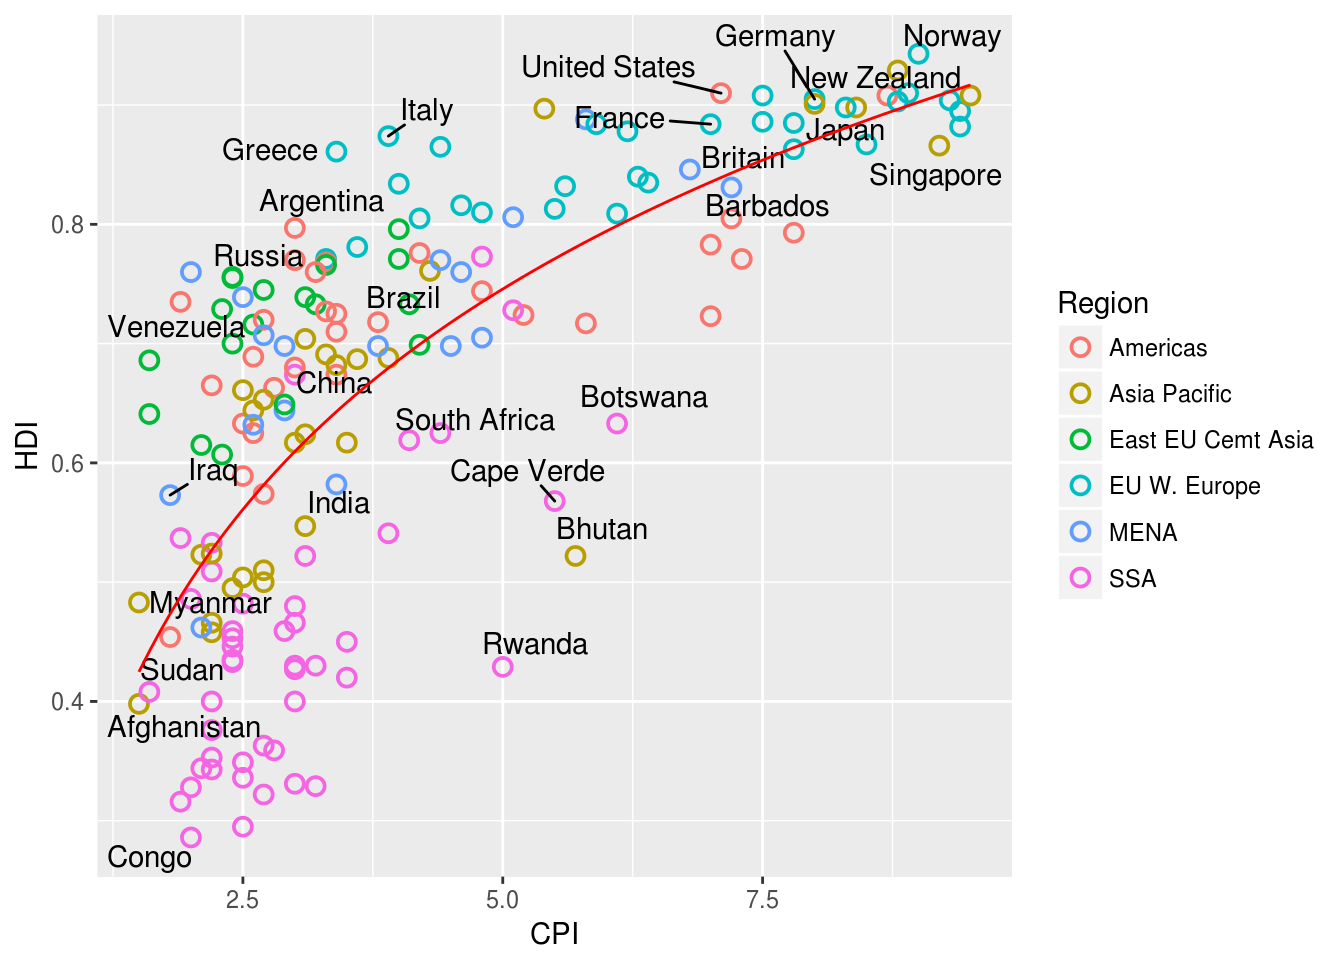
\includegraphics{ggplot_tutorial_files/figure-latex/unnamed-chunk-59-1.pdf}
\item
  Adjust the x and y scales and use \href{http://colorbrewer2.org}{Color
  Brewer} pallete \texttt{Paired}.

  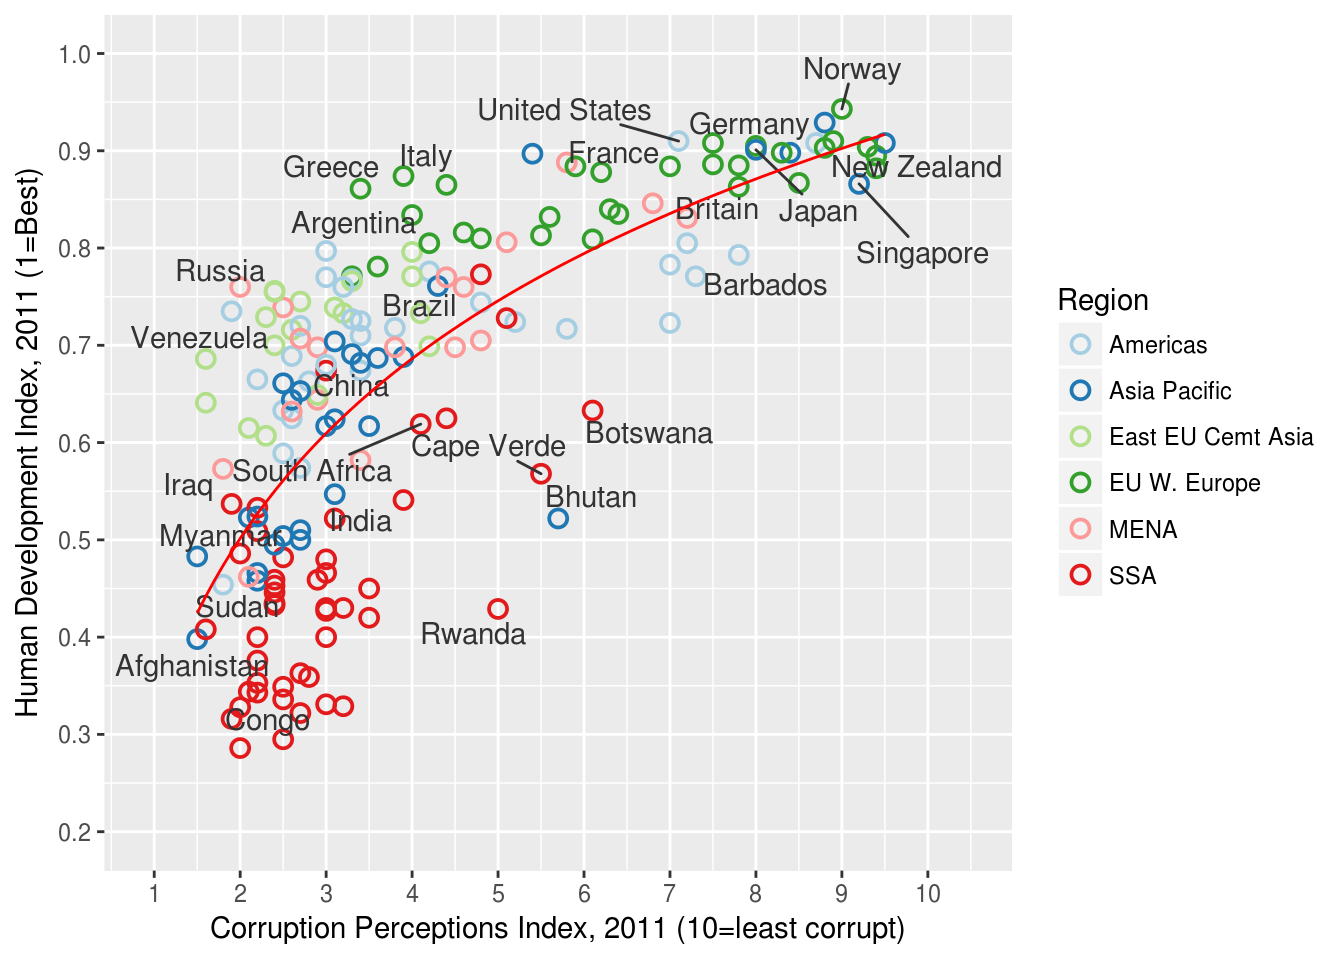
\includegraphics{ggplot_tutorial_files/figure-latex/unnamed-chunk-60-1.pdf}
\item
  Remove vertical grid lines and move the legend

  \includegraphics{ggplot_tutorial_files/figure-latex/unnamed-chunk-61-1.pdf}
\item
  Add title ``Corruption and Human development''

  \includegraphics{ggplot_tutorial_files/figure-latex/unnamed-chunk-62-1.pdf}
\end{enumerate}

\end{document}
